%************************************************
\chapter{Background estimation}
\label{ch:BG}
%************************************************

The charge flip background and the fake lepton background are the two dominant backgrounds due to a mis-reconstruction of the final state leptons.
This type of background will be estimated by using data-driven methods.

\section{Charge flip background}
\label{sec:charge_flip_background}
\subsection{Sources for charge flip background}
The charge flip background is due to the misidentification of the sign of the charge of a lepton.
The sign of the charge is determined by the direction of the curvature of the track.
There are two main sources for the misidentification for the direction of the curvature.

The first source is described by figure \ref{fig:charge_flip_bremsstrahlung}.
It is the case that the lepton interacts with the material of the detector and a photon is emitted by the process of bremsstrahlung.
The emitted photon further produces a pair of electron and positron, namely the $\gamma$ conversion.
As shown in figure \ref{fig:charge_flip_bremsstrahlung}, if most of the energy is carried by the positron $e^{+}$ (the purple track), the direction of the curvature of the reconstructed track (the orange track) will be reversed.
Thus, the charge of the lepton is flipped.
Because the misidentification depends on the amount of the detector material, and hence depends on $|\eta|$ of the original track.

\begin{figure}
\centering
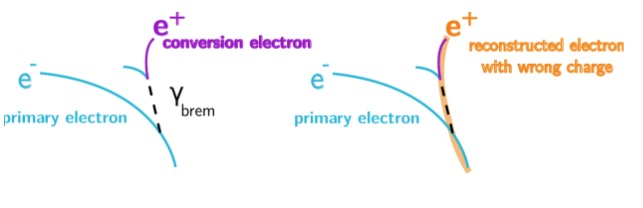
\includegraphics[width=\textwidth]{data/photo/charge_flip/Brem.jpg}
\caption{It shows how the track of the electron is incorrectly reconstructed (the orange track), due to the process of bremsstrahlung and $\gamma$ conversion.}
\label{fig:charge_flip_bremsstrahlung}
\end{figure}

The second source is described by the figure \ref{fig:charge_flip_high_pt}.
When the $p_T$ of the lepton is very high, the track of the lepton will be almost a straight line.
The curvature of the track will be close to zero, and the sign of the curvature will be difficult to be determined.
As a result, the sign of the charge of the lepton is likely incorrectly assigned.
The chance to have this problem obviously depends on $p_T$ of the lepton.

\begin{figure}
\centering
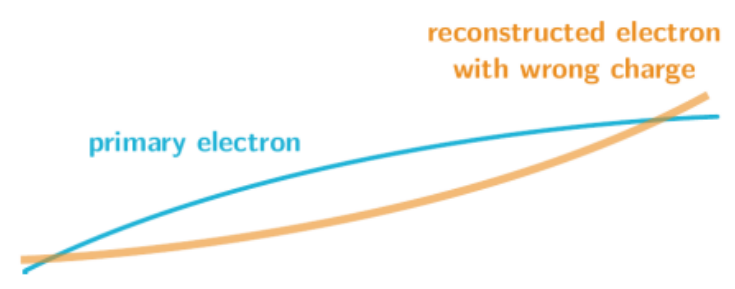
\includegraphics[width=\textwidth]{data/photo/charge_flip/WrongTrack.png}
\caption{It shows how the track of the electron is incorrectly reconstructed (the orange track), due to very high $p_T$ of the electron.}
\label{fig:charge_flip_high_pt}
\end{figure}

Compared to an electron, the charge of a reconstructed muon will be less often to be misidentified.
Firstly, a muon is heavier than an electron.
This will reduce the chance of the process of bremsstrahlung.
Secondly, muons can reach to the muon spectrometer, which is the outer part of the detector, while electrons cannot.
This means that the length of the track of a muon, which can be detected by the tracker, is longer than that of an electron.
Hence, the reconstructed curvature of the track for muons can be more accurate, and it reduces the chance of the misidentification due to the high $p_T$.
Because most of the charge flip background comes from electrons, we only estimate the charge flip background for electrons.

\subsection{Likelihood method}
\label{sec:likelihood_method}
The probability that the charge of an electron is flipped is denoted by the charge-flip rate $\epsilon_i$, where the index i represents the dependency on the $p_T$ and $|\eta|$ of the electron.
The value of index i is found by splitting the variables $p_T$ and $|\eta|$ into different 2-dimensional bins, and the binning for the $p_T$ and $|\eta|$ is described by the table \ref{tab:binning_charge_flip}. The index i of $\epsilon_i$ is defined by the index of the bin.

\begin{table}[htbp]
\centering
\begin{tabular}{|c|c|}
\hline
Variable & Boundary of the bins \\
\hline
$p_T$ (GeV) &  25, 60, 90, 130, 150, 1000 \\
\hline
$|\eta|$ & 0, 0.50, 1.00, 1.37, 1.52, 1.80, 2.00, 2.47 \\
\hline
\end{tabular}
\caption{Binning in $p_T$ and $|\eta|$ for the charge-flip rate $\epsilon_i$.}
\label{tab:binning_charge_flip}
\end{table}

Suppose that there are $m^{ij}_{OS}$ opposite-sign events with the leading lepton in bin $i$ and the sub-leading lepton in bin $j$ before the reconstruction, and there are $m^{ij}_{SS}$ same-sign events.
After the reconstruction, there are $M^{ij}_{OS}$ opposite-sign events and $M^{ij}_{SS}$ same-sign events due to the charge-flipped leptons.
The number of events after the reconstruction is given by
\begin{equation}
M^{ij}_{OS} = (1-\epsilon_i) (1-\epsilon_j) m^{ij}_{OS} + \epsilon_i (1-\epsilon_j) m^{ij}_{SS} + (1-\epsilon_i) \epsilon_j m^{ij}_{SS} + \epsilon_i \epsilon_j m^{ij}_{OS}
\end{equation}
\begin{equation}
M^{ij}_{SS} = (1-\epsilon_i) (1-\epsilon_j) m^{ij}_{SS} + \epsilon_i (1-\epsilon_j) m^{ij}_{OS} + (1-\epsilon_i) \epsilon_j m^{ij}_{OS} + \epsilon_i \epsilon_j m^{ij}_{SS}
\label{equ:MSS}
\end{equation}
From equation \ref{equ:MSS}, the number of reconstructed same-sign events due to the charge-flipped leptons, i.e. the charge flip BG , denoted by $N^{ij}_{SS}$, is
\begin{align}
N^{ij}_{SS}
&= \epsilon_i (1-\epsilon_j) m^{ij}_{OS} + (1-\epsilon_i) \epsilon_j m^{ij}_{OS} + \epsilon_i \epsilon_j m^{ij}_{SS} \\
&\approx \epsilon_i (1-\epsilon_j) m^{ij}_{OS} + (1-\epsilon_i) \epsilon_j m^{ij}_{OS}
\label{equ:NSS}
\end{align}
The dominant charge flip BG comes from events with two opposite-sign electrons, with one of the charge is flipped.
The contribution from the events with two charge-flipped electrons is negligible.

Figure \ref{fig:charge_flip_OS_SS} shows that the number of OS events is much larger than the number of SS events by almost $10^3$ times, and hence $m^{ij}_{OS}$ is much larger than $m^{ij}_{SS}$.
\begin{figure}
\centering
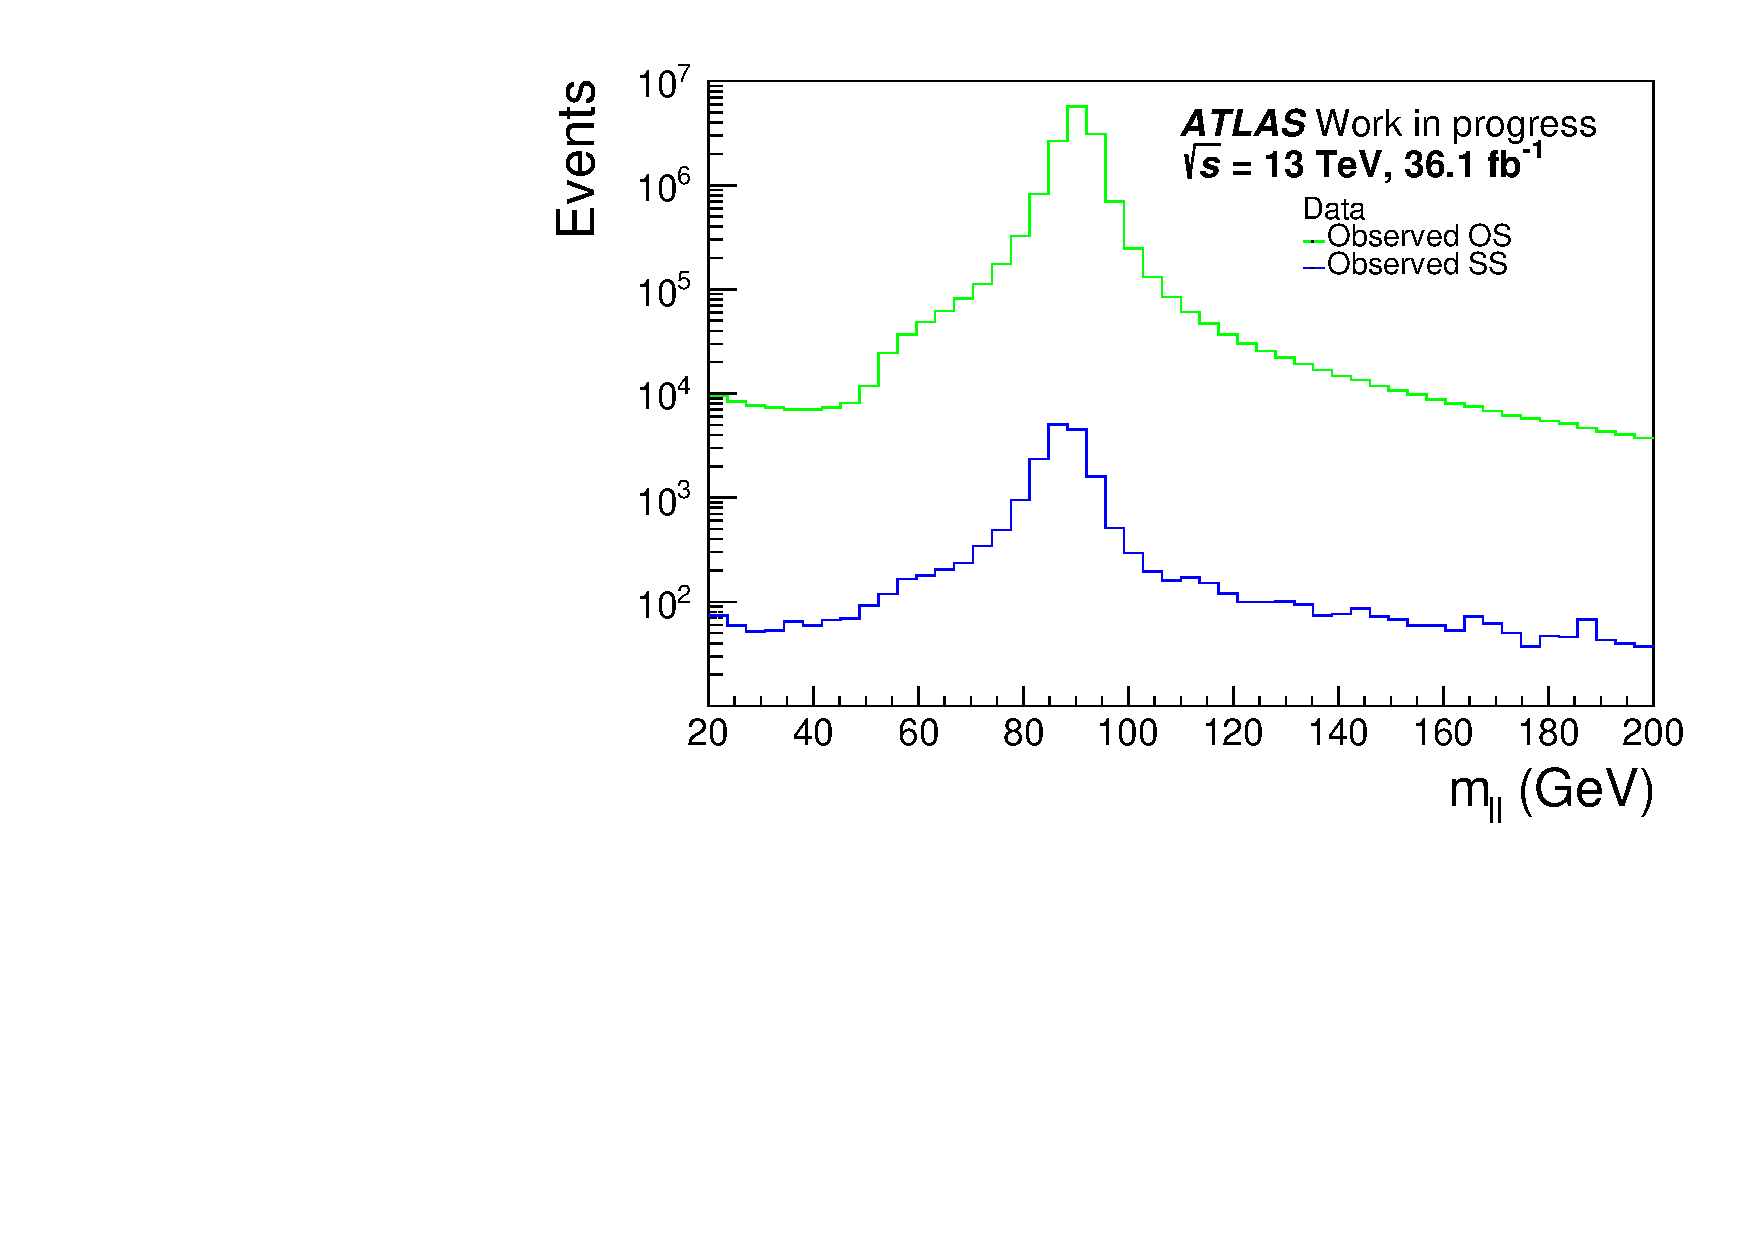
\includegraphics[width=0.9\textwidth]{data/plot/charge_flip/ReweightPlots/plots_NOchfSF/data_mll_unweighted.pdf}
\caption{The comparison between the OS events and the SS events in data. The number of OS events is much larger than the number of SS events by almost $10^3$ times.}
\label{fig:charge_flip_OS_SS}
\end{figure}
Besides, it turns out that the measured charge-flip rate $\epsilon_i$ is about $10^{-3}$, as shown in figure \ref{fig:charge_flip_data_tot}.
Hence, $m^{ij}_{OS}$ can be estimated by
\begin{align}
M^{ij}_{OS} &\approx (1-\epsilon_i) (1-\epsilon_j) m^{ij}_{OS} \\
m^{ij}_{OS} &\approx \frac{ M^{ij}_{OS} }{ (1-\epsilon_i) (1-\epsilon_j) }
\label{equ:mapp1} \\
m^{ij}_{OS} &\approx M^{ij}_{OS} \\
m^{ij}_{OS} &\approx M^{ij}_{OS} + M^{ij}_{SS}
\label{equ:mapp2}
\end{align}
By substituting equation \ref{equ:mapp2} into \ref{equ:NSS}, the charge flip BG can be estimated by $M^{ij}_{OS}$, $M^{ij}_{SS}$ and the charge-flip rate $\epsilon_i$,
\begin{align}
N^{ij}_{SS} &\approx \epsilon_i (1-\epsilon_j) m^{ij}_{OS} + (1-\epsilon_i) \epsilon_j m^{ij}_{OS} \\
&= [ \epsilon_i (1-\epsilon_j) + (1-\epsilon_i) \epsilon_j ] m^{ij}_{OS} \label{equ:NSS3}\\
&\approx p_{ij} (M^{ij}_{OS} + M^{ij}_{SS}) \\
&=p_{ij} N^{ij}
\label{equ:NSS2}
\end{align}
where $p_{ij}$ and $N^{ij}$ are
\begin{align}
\begin{split}
p_{ij} &= \epsilon_i (1-\epsilon_j) + (1-\epsilon_i) \epsilon_j \\
N^{ij} &= M^{ij}_{OS} + M^{ij}_{SS}
\end{split}
\end{align}
The probability density function of $N^{ij}_{SS}$, with the given values of $N^{ij}$ and $\epsilon_i$, can be described by the Poisson distribution with the mean value $\lambda = p_{ij} N^{ij}$.
\begin{align}
P(N^{ij}_{SS}|N^{ij},\epsilon_i,\epsilon_j) &= \frac{ \lambda^{N^{ij}_{SS}} e^{-\lambda} }{N^{ij}_{SS}!} \\
 &= \frac{ (p_{ij} N^{ij})^{N^{ij}_{SS}} e^{- p_{ij} N^{ij}} }{N^{ij}_{SS}!}
\label{equ:poisson}
\end{align}

In order to estimate the charge flip BG, we need to measure the charge-flip rate $\epsilon_i$.
The charge-flip rate is measured as a function of $p_T$ and $|\eta|$ by using a likelihood method, based on the 2015 and 2016 data.
A control region is used to select $Z \rightarrow ee$ processes, with Z mass window of 80 GeV $<m_{ll}<$100 GeV.
Inside the control region, exactly 2 signal electrons are required.
In this control region, the total number of events $N^{ij}$ and the SS events $N^{ij}_{SS}$ in each bin can be measured.
By using the equation \ref{equ:poisson}, the charge-flip rate $\epsilon_i$ can be measured by using the following likelihood method.

The likelihood function $L$ is defined by
\begin{align}
L(\epsilon_i,\epsilon_j|N^{ij},N^{ij}_{SS}) &= \prod_{ij} P(N^{ij}_{SS}|N^{ij},\epsilon_i,\epsilon_j) \\
&= \prod_{ij} \frac{ (p_{ij} N^{ij})^{N^{ij}_{SS}} e^{- p_{ij} N^{ij}} }{N^{ij}_{SS}!}
\end{align}
Given the measured values of $N^{ij}$ and $N^{ij}_{SS}$ in each bin, the value of $\epsilon_i$ can be estimated by maximizing the likelihood function over all possible values of $\epsilon_i$.
By taking the negative logarithm, it is equivalent to minimize $- \ln L$.
\begin{align}
- \ln L
&= - \ln \prod_{ij} \frac{ (p_{ij} N^{ij})^{N^{ij}_{SS}} e^{- p_{ij} N^{ij}} }{N^{ij}_{SS}!} \\
&= - \sum_{ij} \ln \frac{ (p_{ij} N^{ij})^{N^{ij}_{SS}} e^{- p_{ij} N^{ij}} }{N^{ij}_{SS}!} \\
&= - \sum_{ij} \Big[ N^{ij}_{SS} \ln (p_{ij} N^{ij}) - p_{ij} N^{ij} - \ln( N^{ij}_{SS}!) \Big] \\
&= - \sum_{ij} \Big[ N^{ij}_{SS} \ln (p_{ij} N^{ij}) - p_{ij} N^{ij} \Big] + \text{constant} \\
&= - \sum_{ij} \Big[ N^{ij}_{SS} \ln (N^{ij}[\epsilon_i (1-\epsilon_j) + (1-\epsilon_i) \epsilon_j]) - N^{ij}[\epsilon_i (1-\epsilon_j) + (1-\epsilon_i) \epsilon_j] \Big] + \text{constant}
\end{align}

\subsection{Background subtraction}
\label{sec:Background_subtraction}
By minimizing $- \ln L$ described in the previous section, the value of the charge-flip rate $\epsilon_i$ can be measured by using the data in the control region.
In order to have accurate $N^{ij}$ and $N^{ij}_{SS}$, the number of events should come from $Z \rightarrow ee$ processes, and other processes should be subtracted in data.
The number of events from other processes can be estimated with the sideband method in the region: 60 GeV $<m_{ll}<$ 80 GeV and 100 GeV $<m_{ll}<$ 120 GeV, by assuming a flat distribution.
The corrected values of $N^{ij}$ and $N^{ij}_{SS}$ are given by
\begin{align}
N_{80,100;\text{corrected}} = N_{80,100} - 20 \Big( \frac{N_{60,80} + N_{80,100}}{20 + 20} \Big)
\end{align}
In the sideband subtraction, the number of events in the sideband region should be normalized to the width of the central region.
In general, given the number of events in the central region $N_{\text{central}}$, the left sideband region $N_{\text{left}}$ and the right sideband region $N_{\text{right}}$, and their corresponding width $w_{\text{central}}$, $w_{\text{left}}$ and $w_{\text{right}}$, the corrected values $N_{\text{central,corrected}}$ are given by
\begin{align}
N_{\text{central,corrected}} = N_{\text{central}} - w_{\text{central}} \Big( \frac{N_{\text{left}} + N_{\text{right}}}{w_{\text{left}} + w_{\text{right}}} \Big)
\end{align}

\subsection{Results without systematic uncertainty}
\label{sec:results_stat}
Figure \ref{fig:charge_flip_data_stat} shows the measured values of the charge-flip rate $\epsilon_i$ by using the data.
The errors only include the uncertainties in the likelihood method due to the statistics, denoted by $\epsilon_{\text{lik,data}}$.

\begin{figure}
\centering
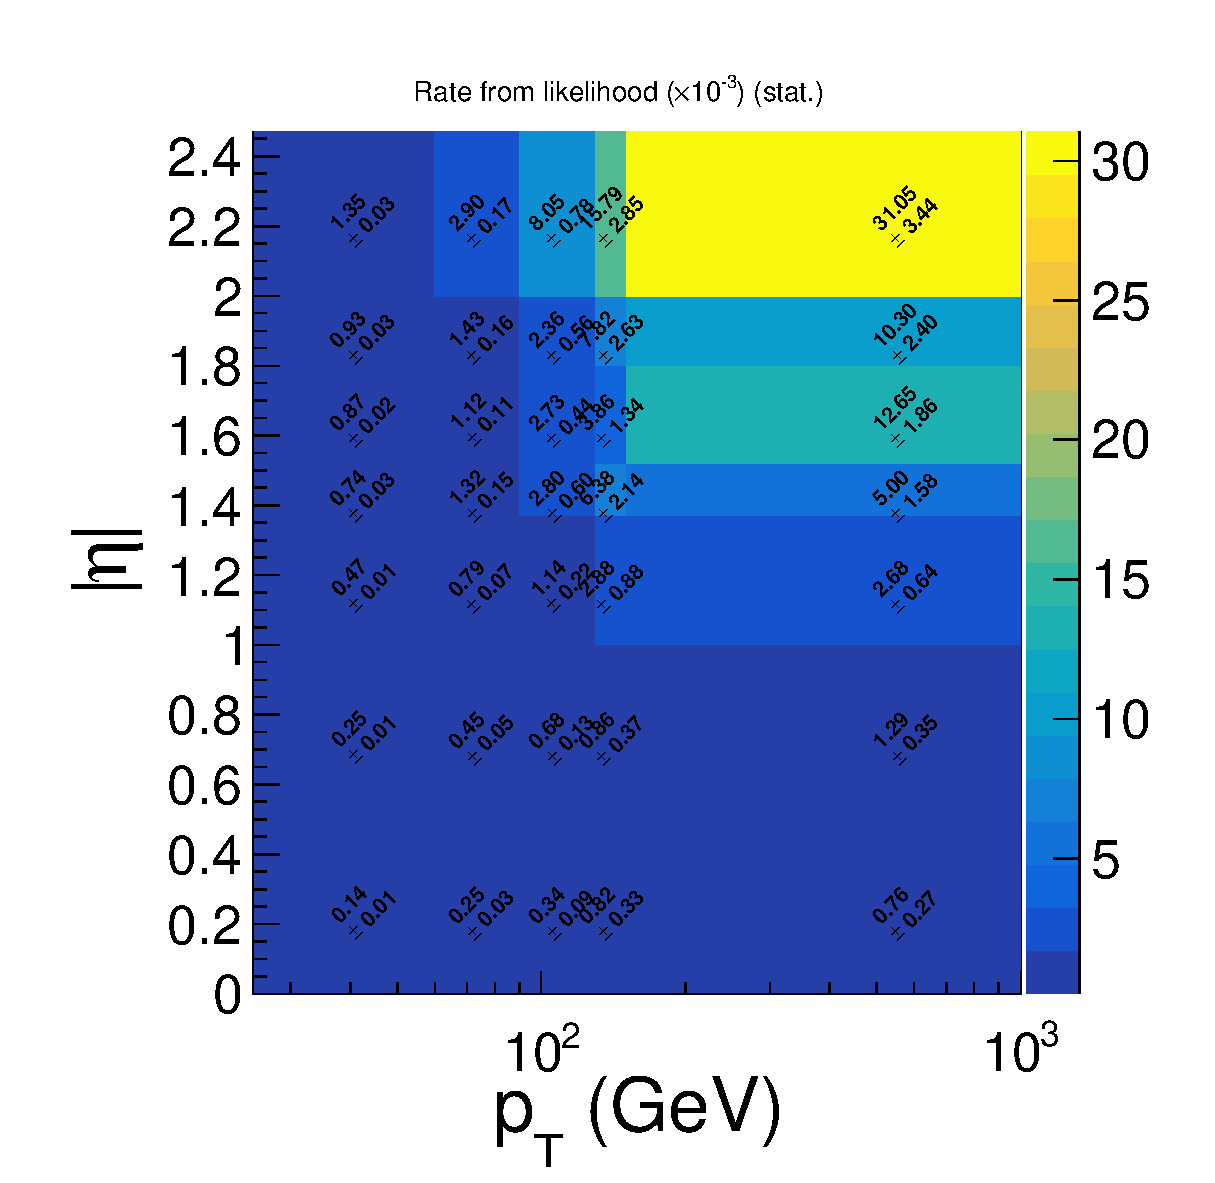
\includegraphics[width=\textwidth]{data/plot/charge_flip/FitPlots/data_cf_rate_stat.eps}
\caption{The measured values of the charge-flip rate $\epsilon_i$ in data. Only uncertainties due to the likelihood method are included.}
\label{fig:charge_flip_data_stat}
\end{figure}

\subsection{Systematic uncertainties due to background subtraction}
\label{sec:sys_background_subtraction}
The systematic uncertainties due to background subtraction is estimated by the variations of different central widths and sideband widths.
The following are the nominal central region and sideband region, and their 4 variations. \\
The nominal background subtraction:
\begin{itemize}
\item Central region: 80 - 100 GeV; Sideband width: 20 GeV
\end{itemize}
The 4 variations for background subtraction:
\begin{itemize}
\item Central region: 80 - 100 GeV; Sideband width: 15 GeV
\item Central region: 80 - 100 GeV; Sideband width: 25 GeV
\item Central region: 75 - 105 GeV; Sideband width: 20 GeV
\item Central region: 80 - 100 GeV; no background subtraction
\end{itemize}

For each bin, the largest deviation from the nominal among these variations is the systematic uncertainty due to background subtraction.
\begin{equation}
\sigma_{\text{bgk}} = \max \{| \sigma_{\text{nominal}} - \sigma_{\text{variation}} |\}
\end{equation}

Figure \ref{fig:charge_flip_sys_background_subtraction} shows the variations of the resulting charge flip rate, due to these 4 variations.
\begin{figure}
\centering
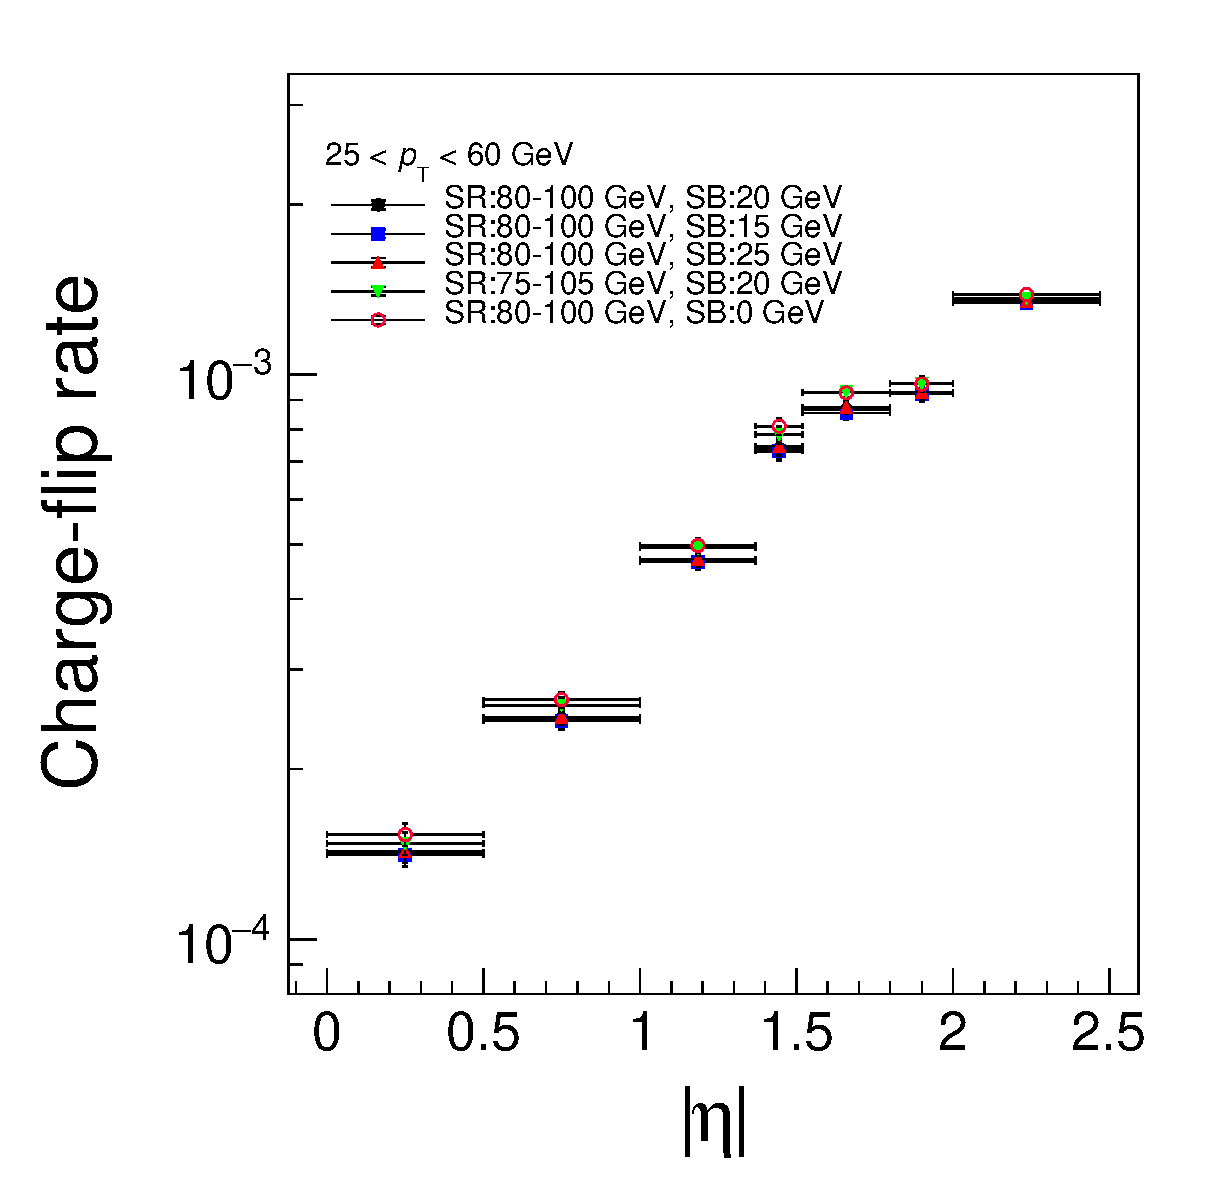
\includegraphics[width=0.3\textwidth]{data/plot/charge_flip/FitPlots/data_cf_comparison_0.eps}
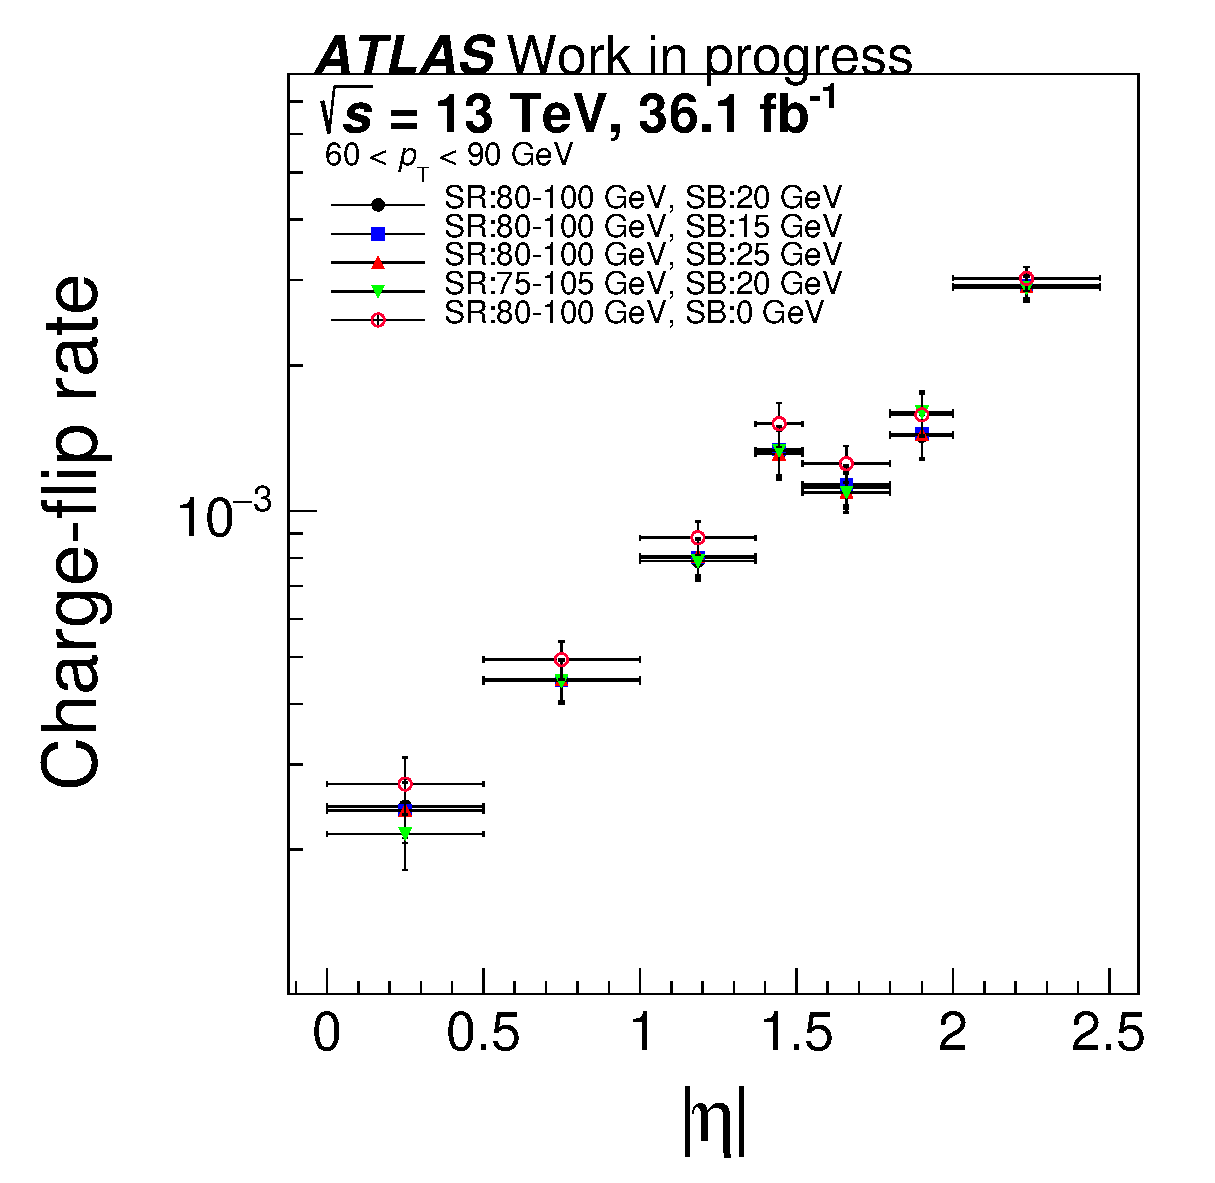
\includegraphics[width=0.3\textwidth]{data/plot/charge_flip/FitPlots/data_cf_comparison_1.eps}
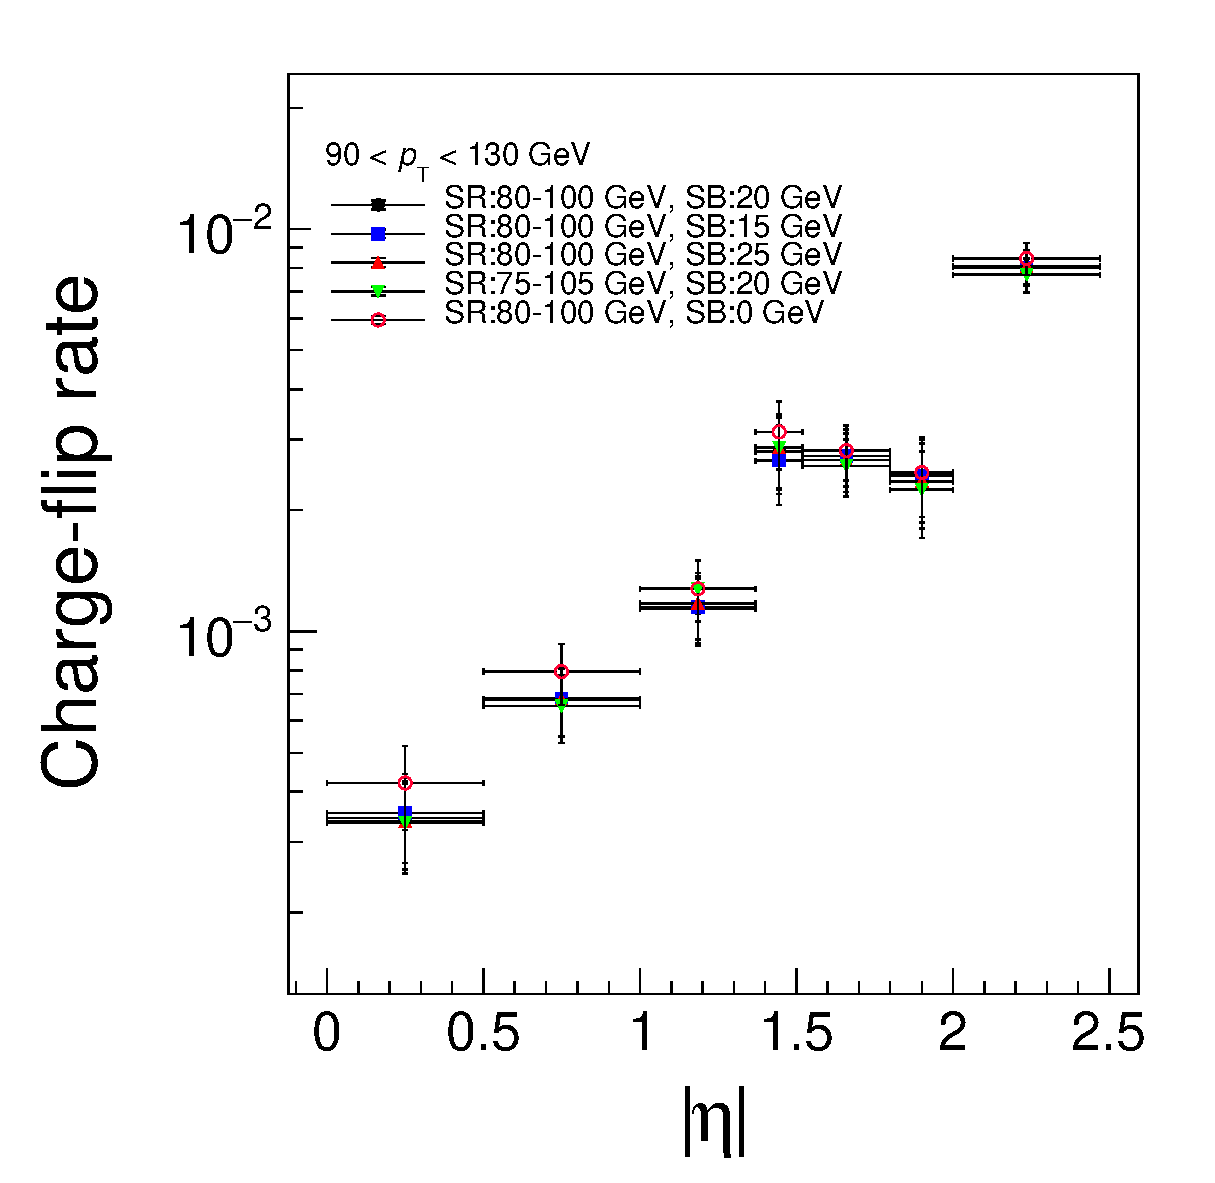
\includegraphics[width=0.3\textwidth]{data/plot/charge_flip/FitPlots/data_cf_comparison_2.eps} \\
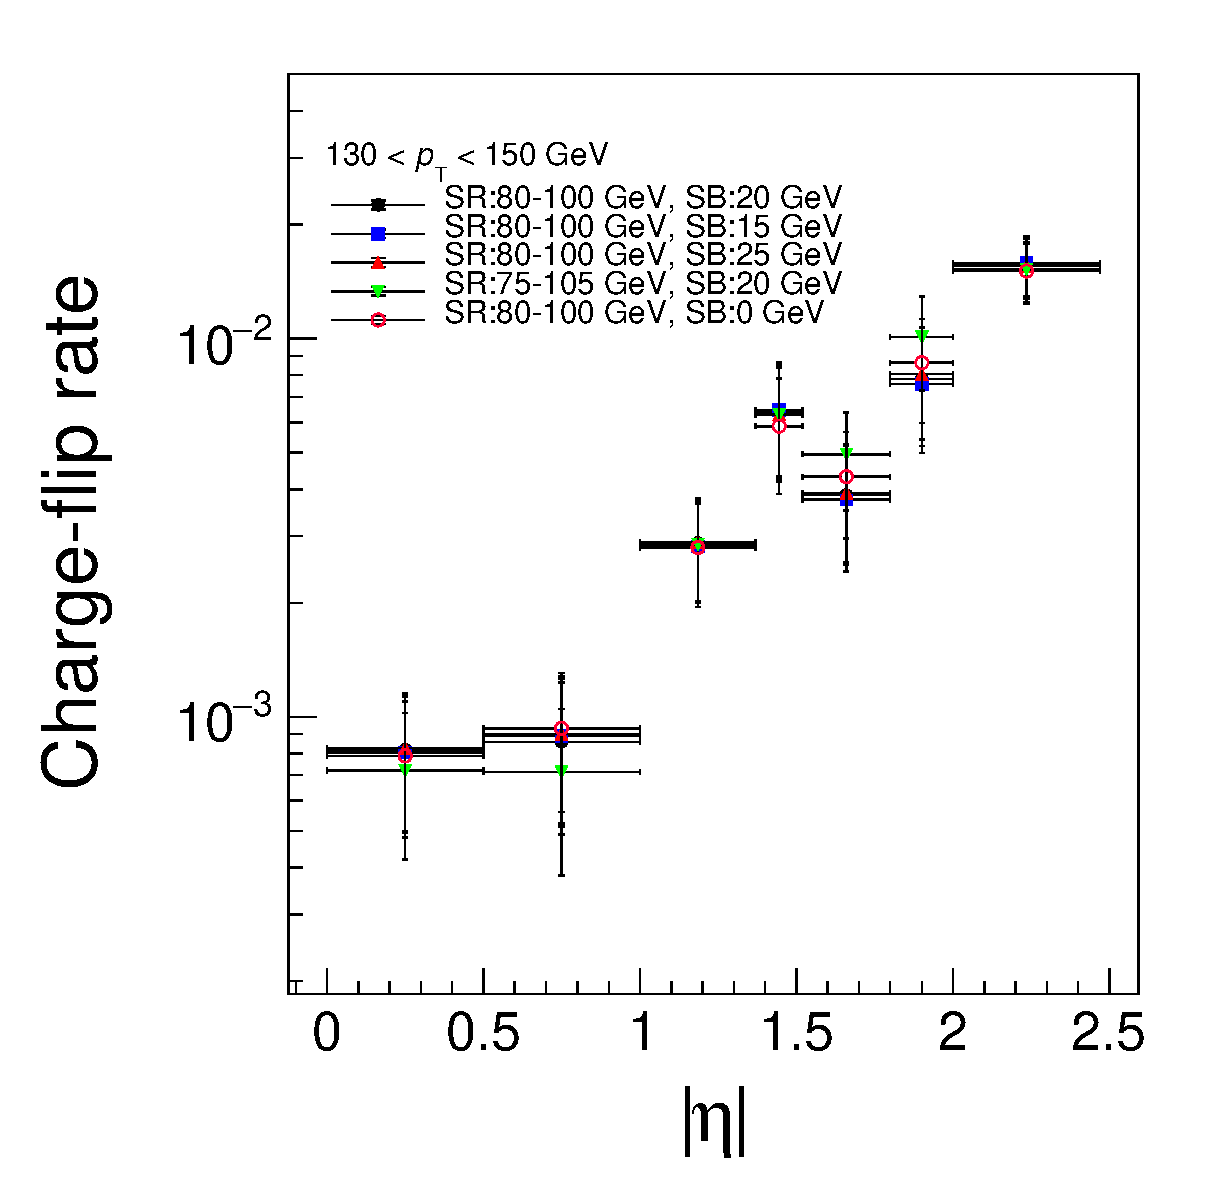
\includegraphics[width=0.3\textwidth]{data/plot/charge_flip/FitPlots/data_cf_comparison_3.eps}
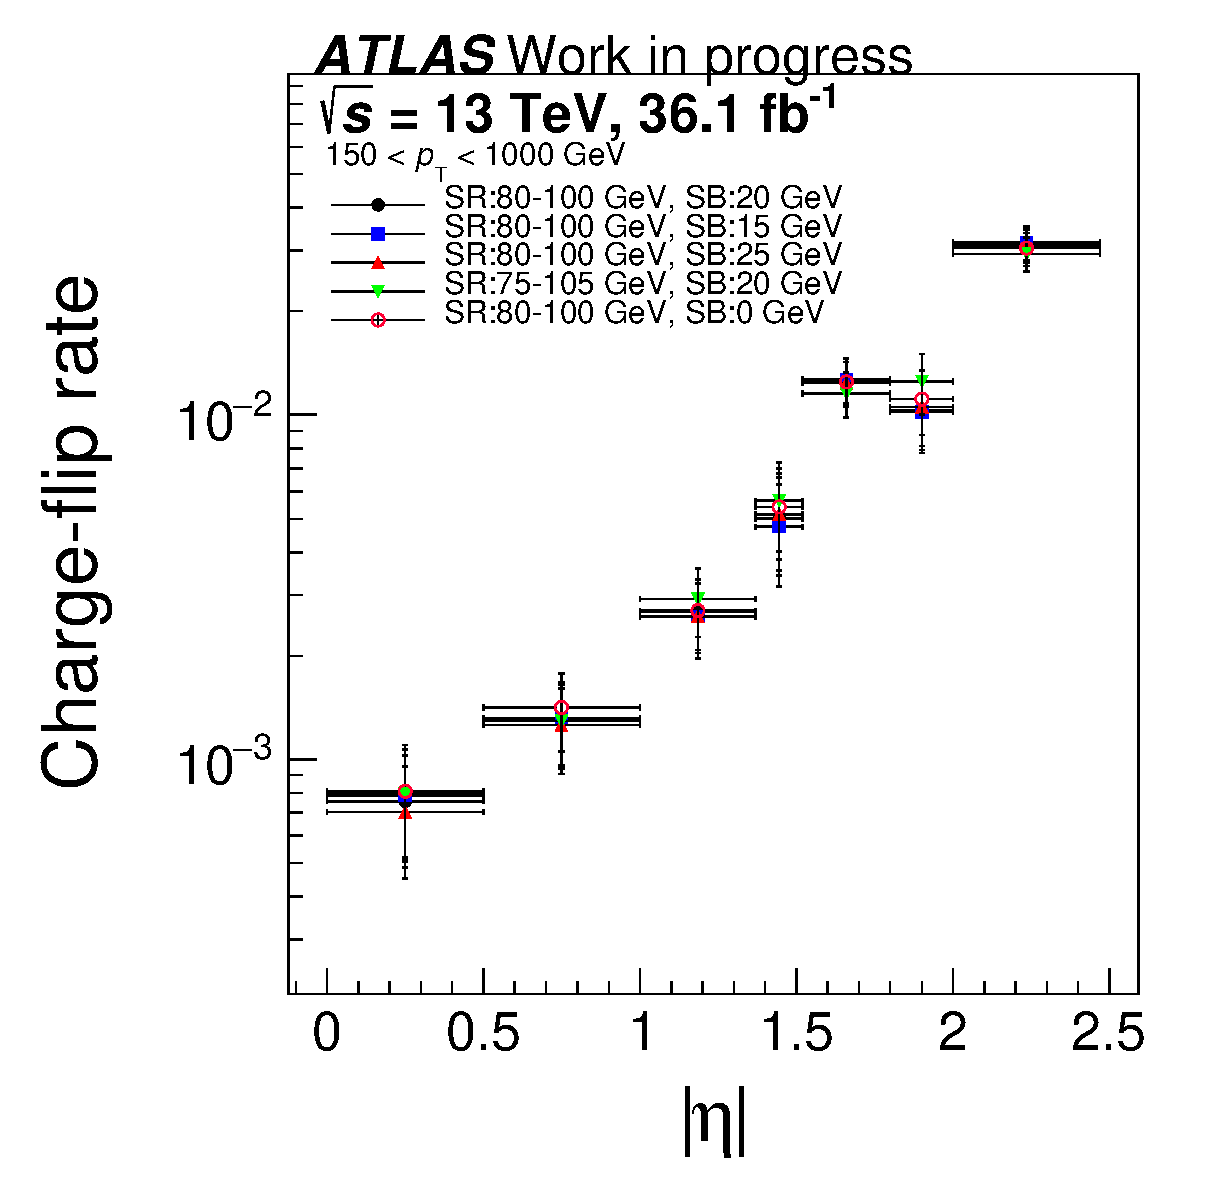
\includegraphics[width=0.3\textwidth]{data/plot/charge_flip/FitPlots/data_cf_comparison_4.eps}
\caption{The systematic variations of the charge-flip rate $\epsilon_i$ in data, due to the background subtraction.}
\label{fig:charge_flip_sys_background_subtraction}
\end{figure}

\subsection{Systematic uncertainties due to likelihood method}
\label{sec:sys_likelihood}
The systematic uncertainties due to likelihood method are estimated by the difference between the likelihood method and the MC truth method.
In the MC truth method, the charge-flip rate is estimated by using the truth information in the $Z \rightarrow ee$ MC sample inside the control region.
The control region requires exactly 2 signal electrons.
The following are the procedures to match the reconstructed electron to the original electron, in order to find out the original electric charge.
In this procedure, some reconstructed electrons cannot be matched.
Figure \ref{fig:charge_flip_MC_match} shows how the original electron is found in the decay process described in figure \ref{fig:charge_flip_bremsstrahlung}.
\begin{figure}
\centering
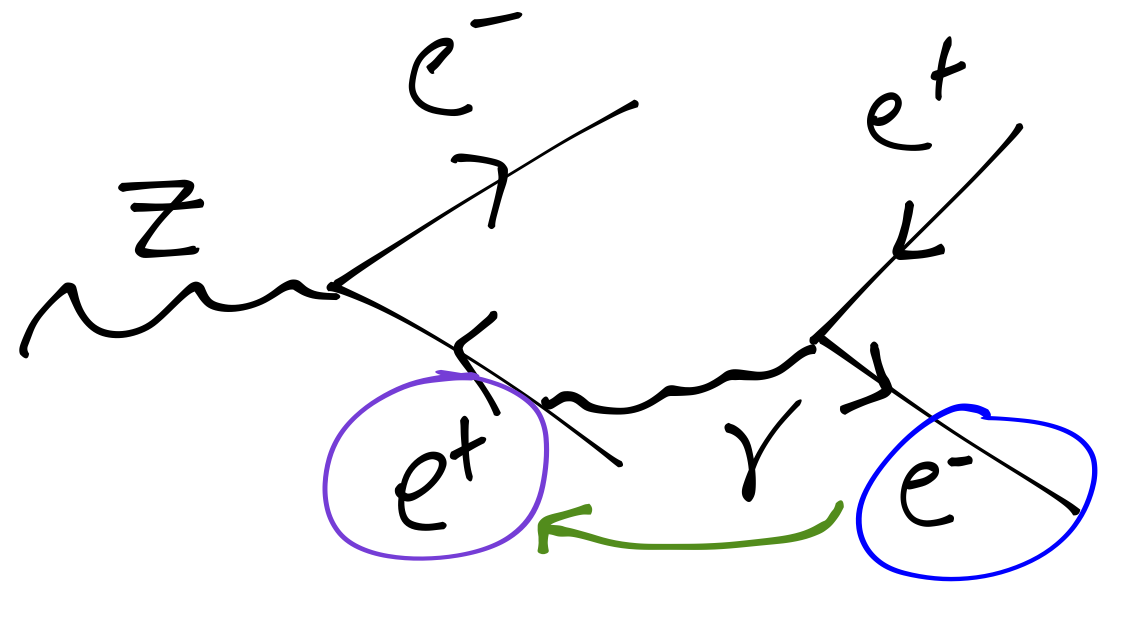
\includegraphics[width=0.5\textwidth]{data/photo/charge_flip/MC-truth.png}
\caption{This diagram shows how the original electron is found through the decay chain.}
\label{fig:charge_flip_MC_match}
\end{figure}
\begin{enumerate}
\item The reconstructed electron will be matched to the truth particle with the smallest $\Delta R$ within the cone $\Delta R < 0.1$.
\item In the following cases, the reconstructed electron are thrown away.
\begin{enumerate}
\item No any truth particles can be found inside the cone.
\item The truth particle is not an electron.
\item The origin of the truth electron is not a Z boson.
\item The daughter particle of the Z boson is not an electron.
\end{enumerate}
\item The charge of the daughter electron from the Z boson is the original charge of the reconstructed electron.
\end{enumerate}

Only the events with two reconstructed electrons that are kept in the above procedure are considered.
$N_{\text{total}}$ is the total number of electrons in these events, and $N_{\text{flipped}}$ is the number of electrons that the original charge and the reconstructed charge are different.
By calculating the ratio in each bin, the charge flip rate can be estimated by using the MC truth information.
\begin{equation}
\epsilon_{\text{MC truth}} = \frac{N_{\text{flipped}}}{N_{\text{total}}}
\end{equation}

The systematic uncertainties due to likelihood method $\sigma_{\text{truth}}$ is then given by \\
for MC,
\begin{equation}
\sigma_{\text{truth,MC}} = | \epsilon_{\text{lik,MC}} - \epsilon_{\text{MC truth}} |
\end{equation}
for data,
\begin{equation}
\sigma_{\text{truth,data}} = \epsilon_{\text{lik,data}} \times \frac{\sigma_{\text{truth,MC}}}{\epsilon_{\text{lik,MC}}}
\end{equation}

Figure \ref{fig:charge_flip_sys_truth} shows the comparison of the resulting charge flip rate, between the likelihood method and the MC truth method.
\begin{figure}
\centering
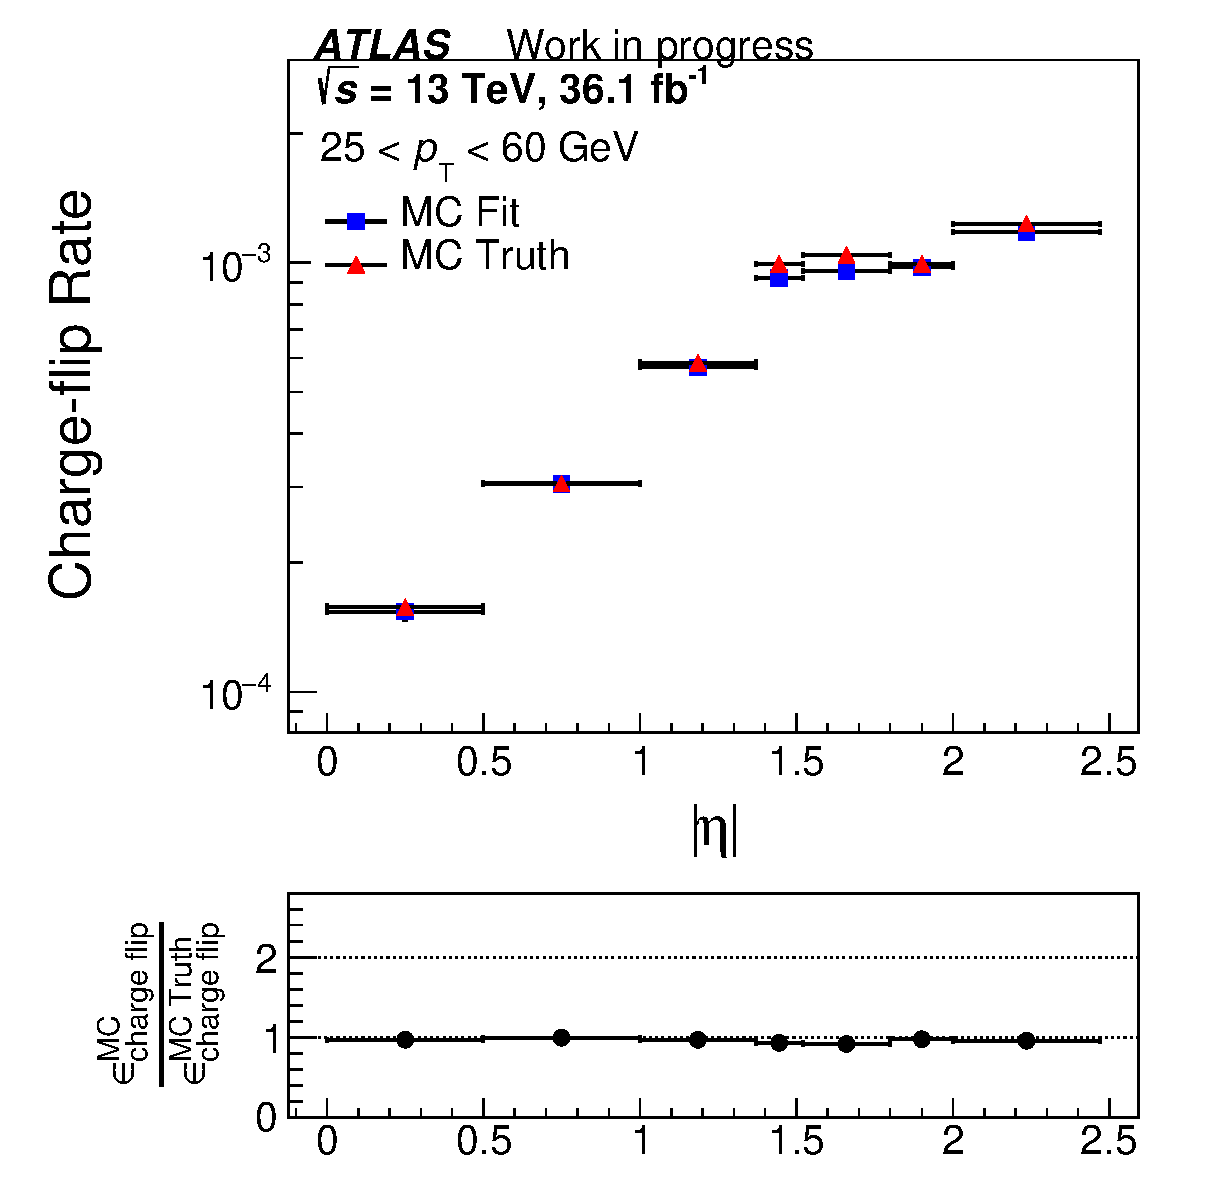
\includegraphics[width=0.3\textwidth]{data/plot/charge_flip/FitPlots/mc_cf_rate_0.eps}
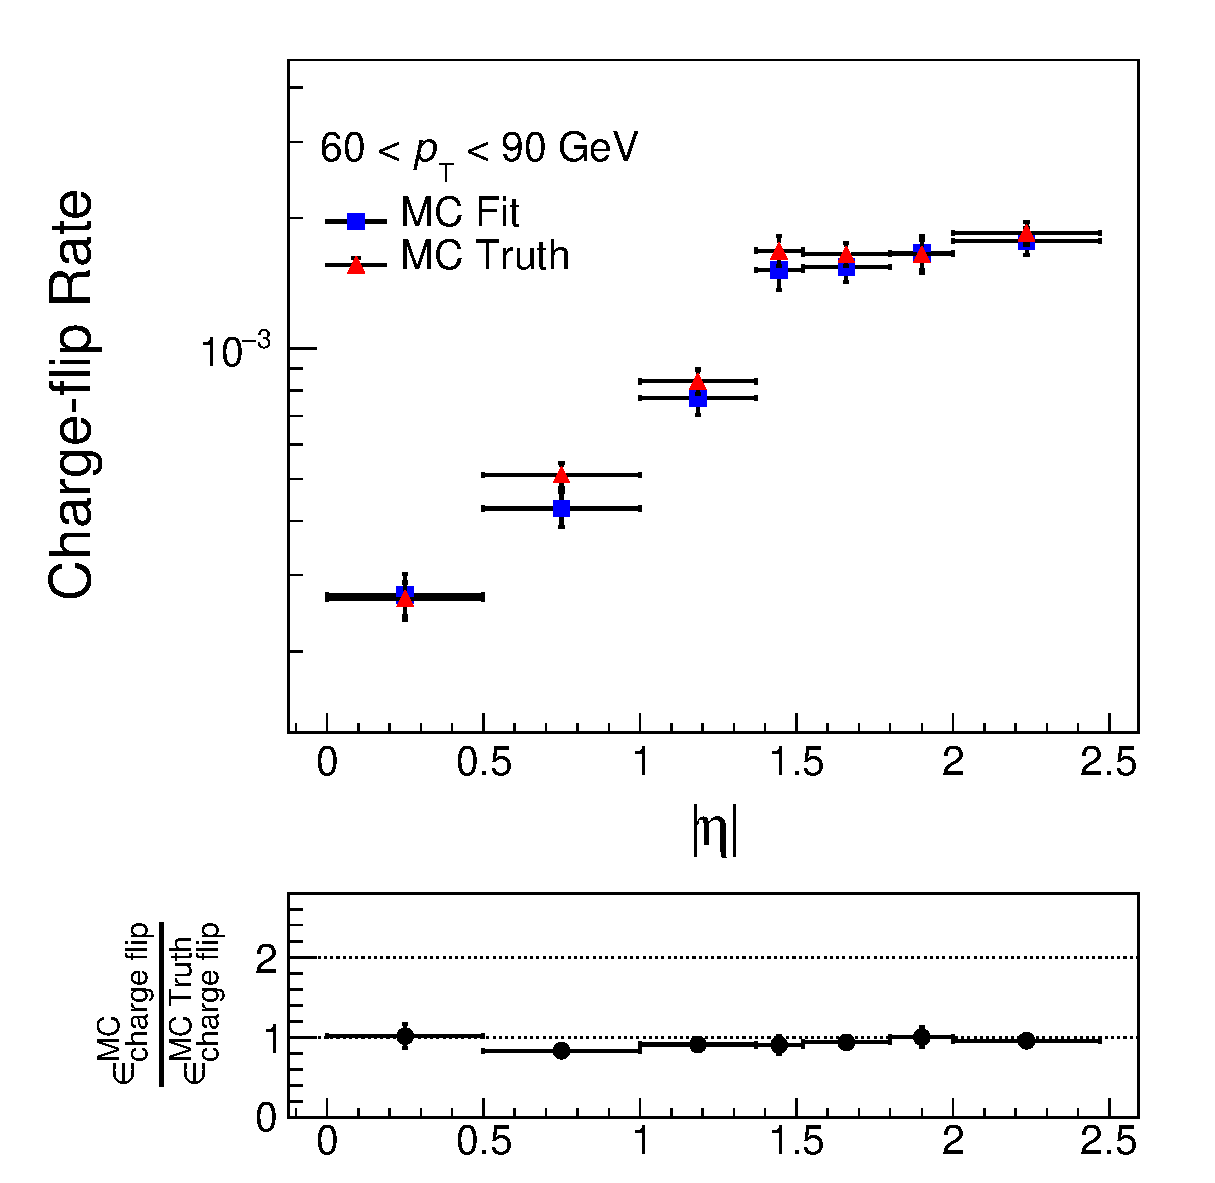
\includegraphics[width=0.3\textwidth]{data/plot/charge_flip/FitPlots/mc_cf_rate_1.eps}
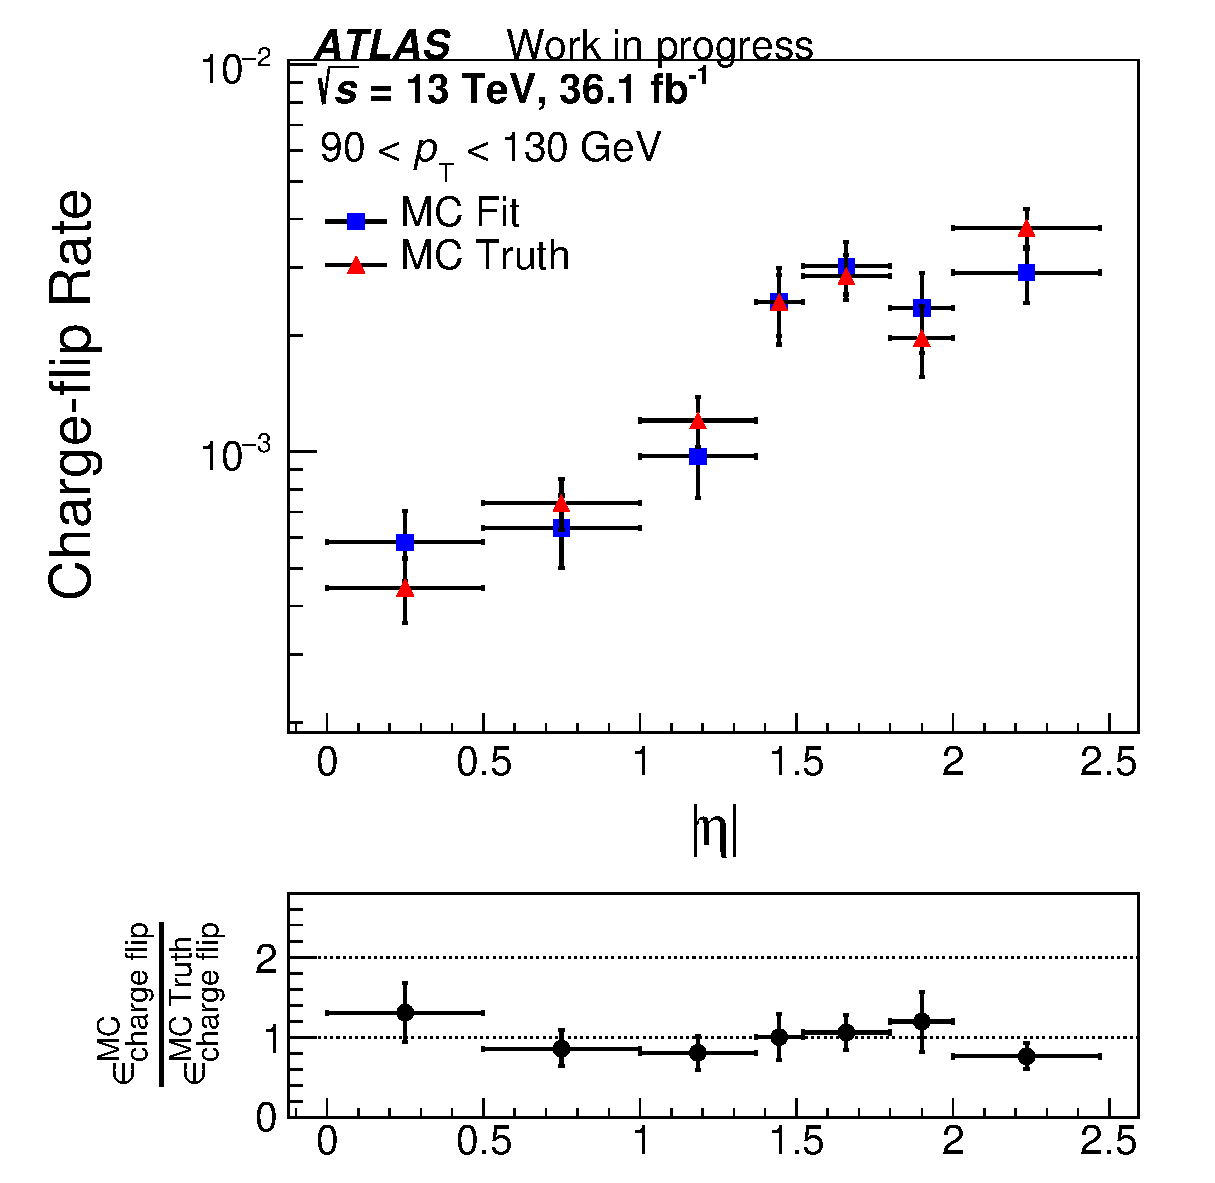
\includegraphics[width=0.3\textwidth]{data/plot/charge_flip/FitPlots/mc_cf_rate_2.eps} \\
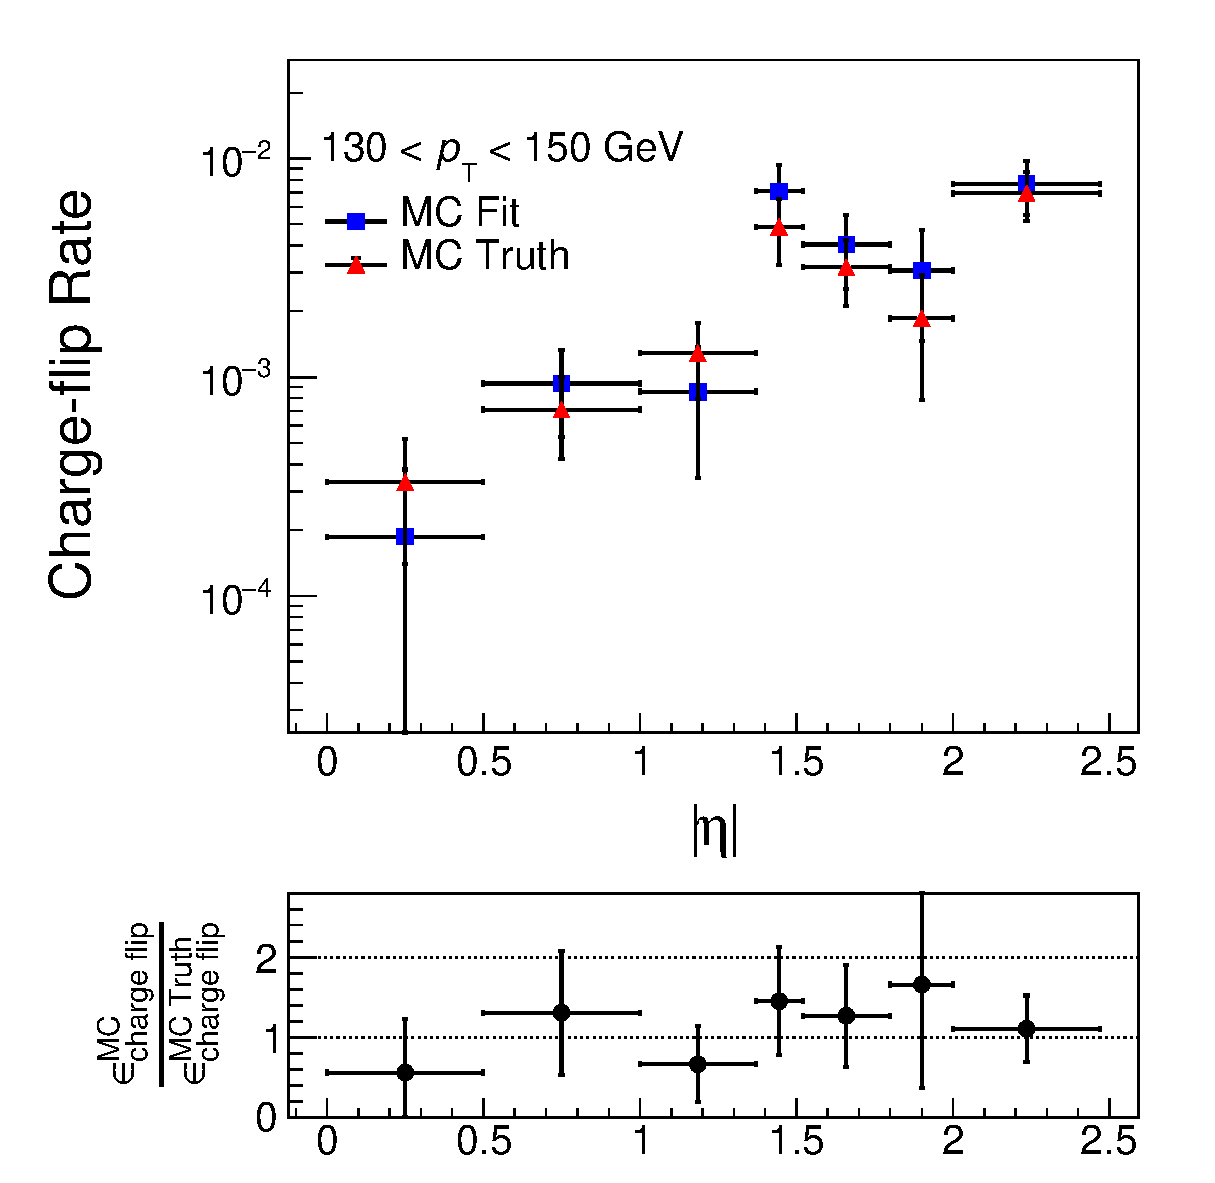
\includegraphics[width=0.3\textwidth]{data/plot/charge_flip/FitPlots/mc_cf_rate_3.eps}
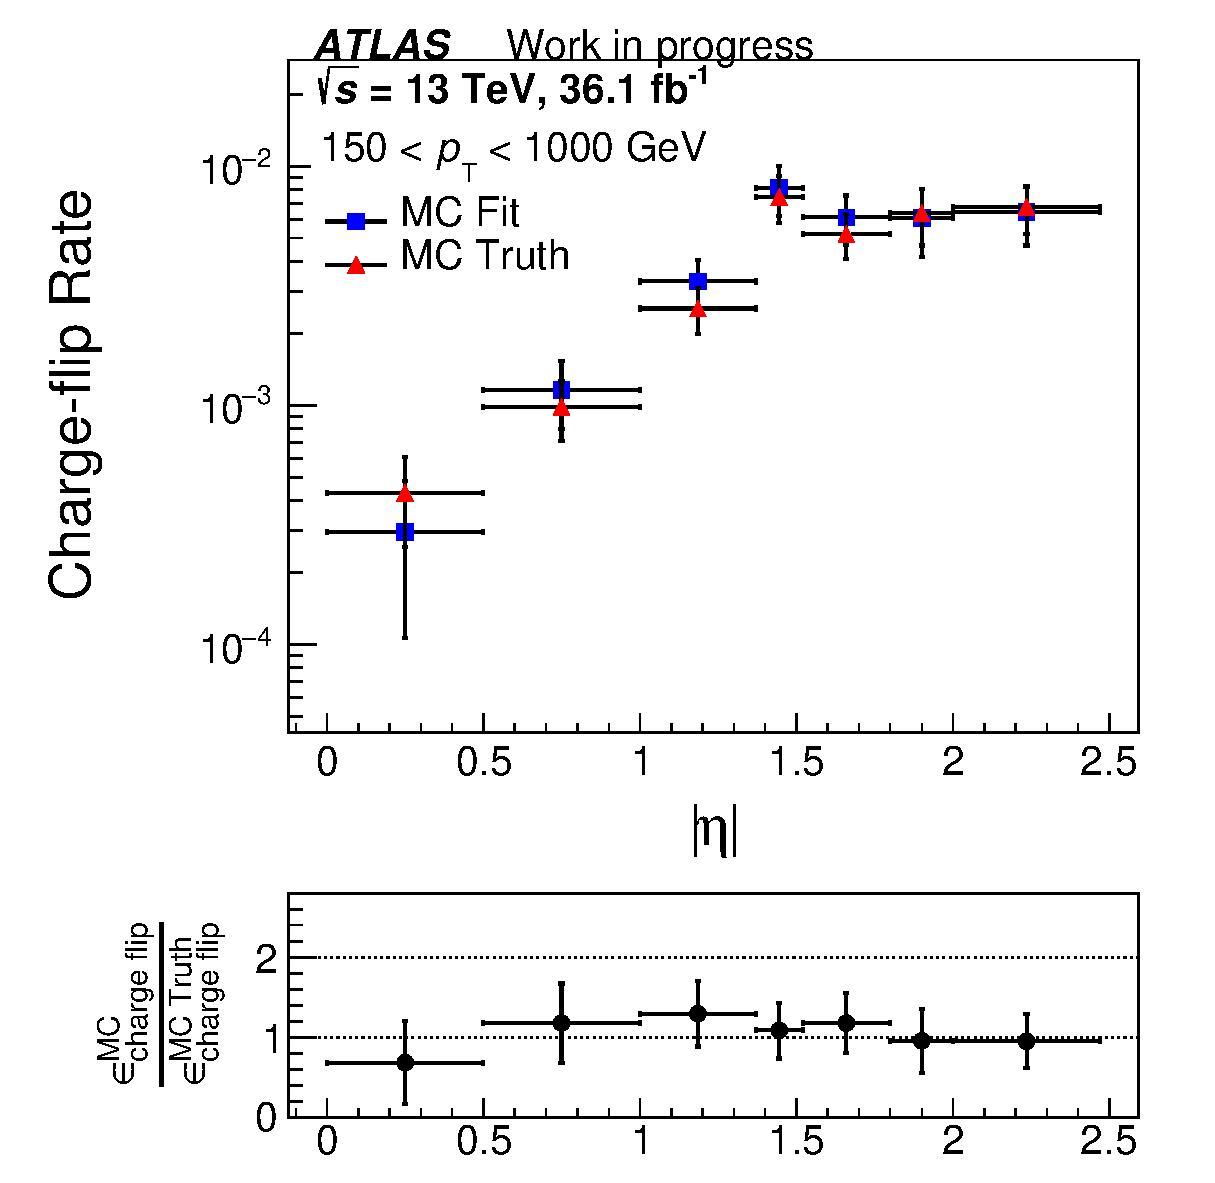
\includegraphics[width=0.3\textwidth]{data/plot/charge_flip/FitPlots/mc_cf_rate_4.eps}
\caption{The comparisons between the likelihood method and the MC truth method. The systematic uncertainties due to likelihood method can be estimated.}
\label{fig:charge_flip_sys_truth}
\end{figure}

\subsection{Results with total uncertainties}
\label{sec:charge_flip_results_stat}
The total systematic uncertainties is a quadratic sum of systematic uncertainties due to the background subtraction and the likelihood method, described in section \ref{sec:sys_background_subtraction} and \ref{sec:sys_likelihood} respectively.
\begin{equation}
\sigma_{\text{sys}} = \sqrt{\sigma_{\text{bgk}} ^2+ \sigma_{\text{truth}} ^2}
\end{equation}
The total uncertainties is the quadratic sum of the total systematic uncertainties and the statistical uncertainties in the likelihood method.
\begin{equation}
\sigma_{\text{tot}} = \sqrt{\sigma_{\text{sys}} ^2 + \sigma_{\text{lik}} ^2}
\label{equ:tot_error}
\end{equation}

Figure \ref{fig:charge_flip_data_tot} shows the measured values of the charge-flip rate $\epsilon_i$ by using the data, with total uncertainties described in equation \ref{equ:tot_error}.

\begin{figure}
\centering
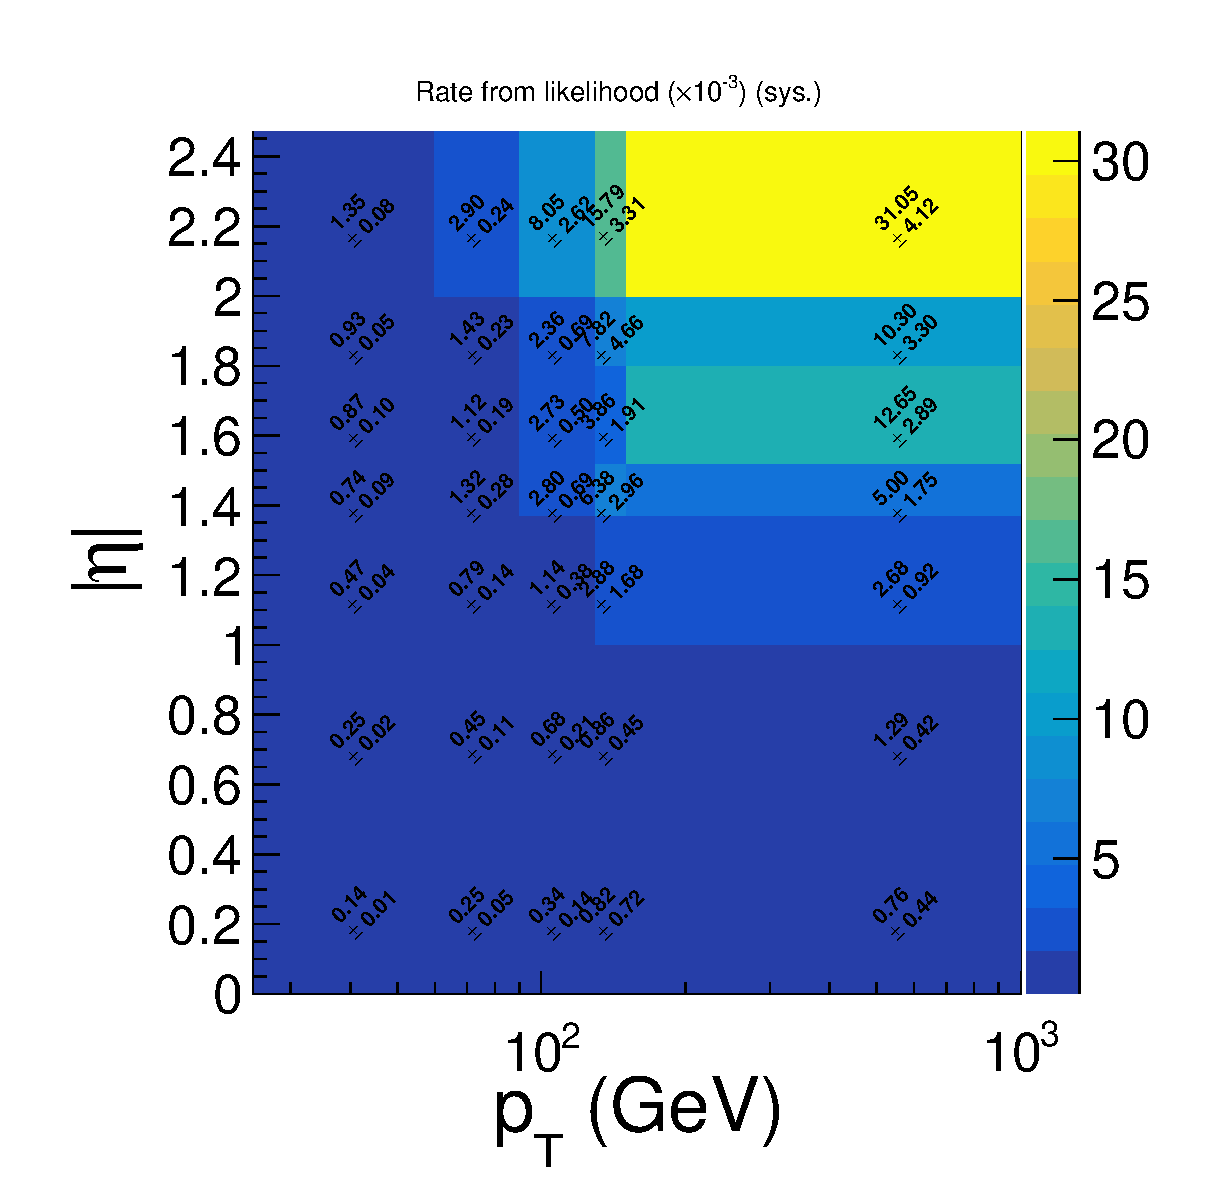
\includegraphics[width=\textwidth]{data/plot/charge_flip/FitPlots/data_cf_rate_tot.eps}
\caption{The measured values of the charge-flip rate $\epsilon_i$ in data, with total uncertainties.}
\label{fig:charge_flip_data_tot}
\end{figure}

\subsection{MC validation}
\label{sec:charge_flip_MC_validation}
The charge flip rate can be validated by using the $Z \rightarrow ee$ MC samples.
By using the equation \ref{equ:mapp1} and \ref{equ:NSS3}, $N^{ij}_{SS}$ can be approximated by
\begin{align}
N^{ij}_{SS} &= [ \epsilon_i (1-\epsilon_j) + (1-\epsilon_i) \epsilon_j ] m^{ij}_{OS} \\
&\approx [ \epsilon_i (1-\epsilon_j) + (1-\epsilon_i) \epsilon_j ] \frac{ M^{ij}_{OS} }{ (1-\epsilon_i) (1-\epsilon_j) } \\
&= \frac{\epsilon_i (1-\epsilon_j) + (1-\epsilon_i) \epsilon_j}{(1-\epsilon_i) (1-\epsilon_j)} M^{ij}_{OS}
\end{align}
In the equation \ref{equ:MSS}, $m^{ij}_{SS}$ is zero for the $Z \rightarrow ee$ MC samples, therefore we have
\begin{align}
M^{ij}_{SS} &= \epsilon_i (1-\epsilon_j) m^{ij}_{OS} + (1-\epsilon_i) \epsilon_j m^{ij}_{OS} \\
&= N^{ij}_{SS}
\end{align}
Hence, it is expected that
\begin{align}
M^{ij}_{SS} \approx \frac{\epsilon_i (1-\epsilon_j) + (1-\epsilon_i) \epsilon_j}{(1-\epsilon_i) (1-\epsilon_j)} M^{ij}_{OS}
\end{align}
By weighting the OS events in MC with the weight,
\begin{align}
\text{weight} = \frac{\epsilon_i (1-\epsilon_j) + (1-\epsilon_i) \epsilon_j}{(1-\epsilon_i) (1-\epsilon_j)}
\end{align}
the weighted OS events and the SS events will be close to each other.
This can be used to validate the charge flip rate.
Figure \ref{fig:charge_flip_MC_validation} shows the comparisons between the weighted OS events and the SS events in various distributions, where all event weights are applied except the charge flip scale factor.
The weighted OS events and the SS events agree within the uncertainties.
\begin{figure}
\centering
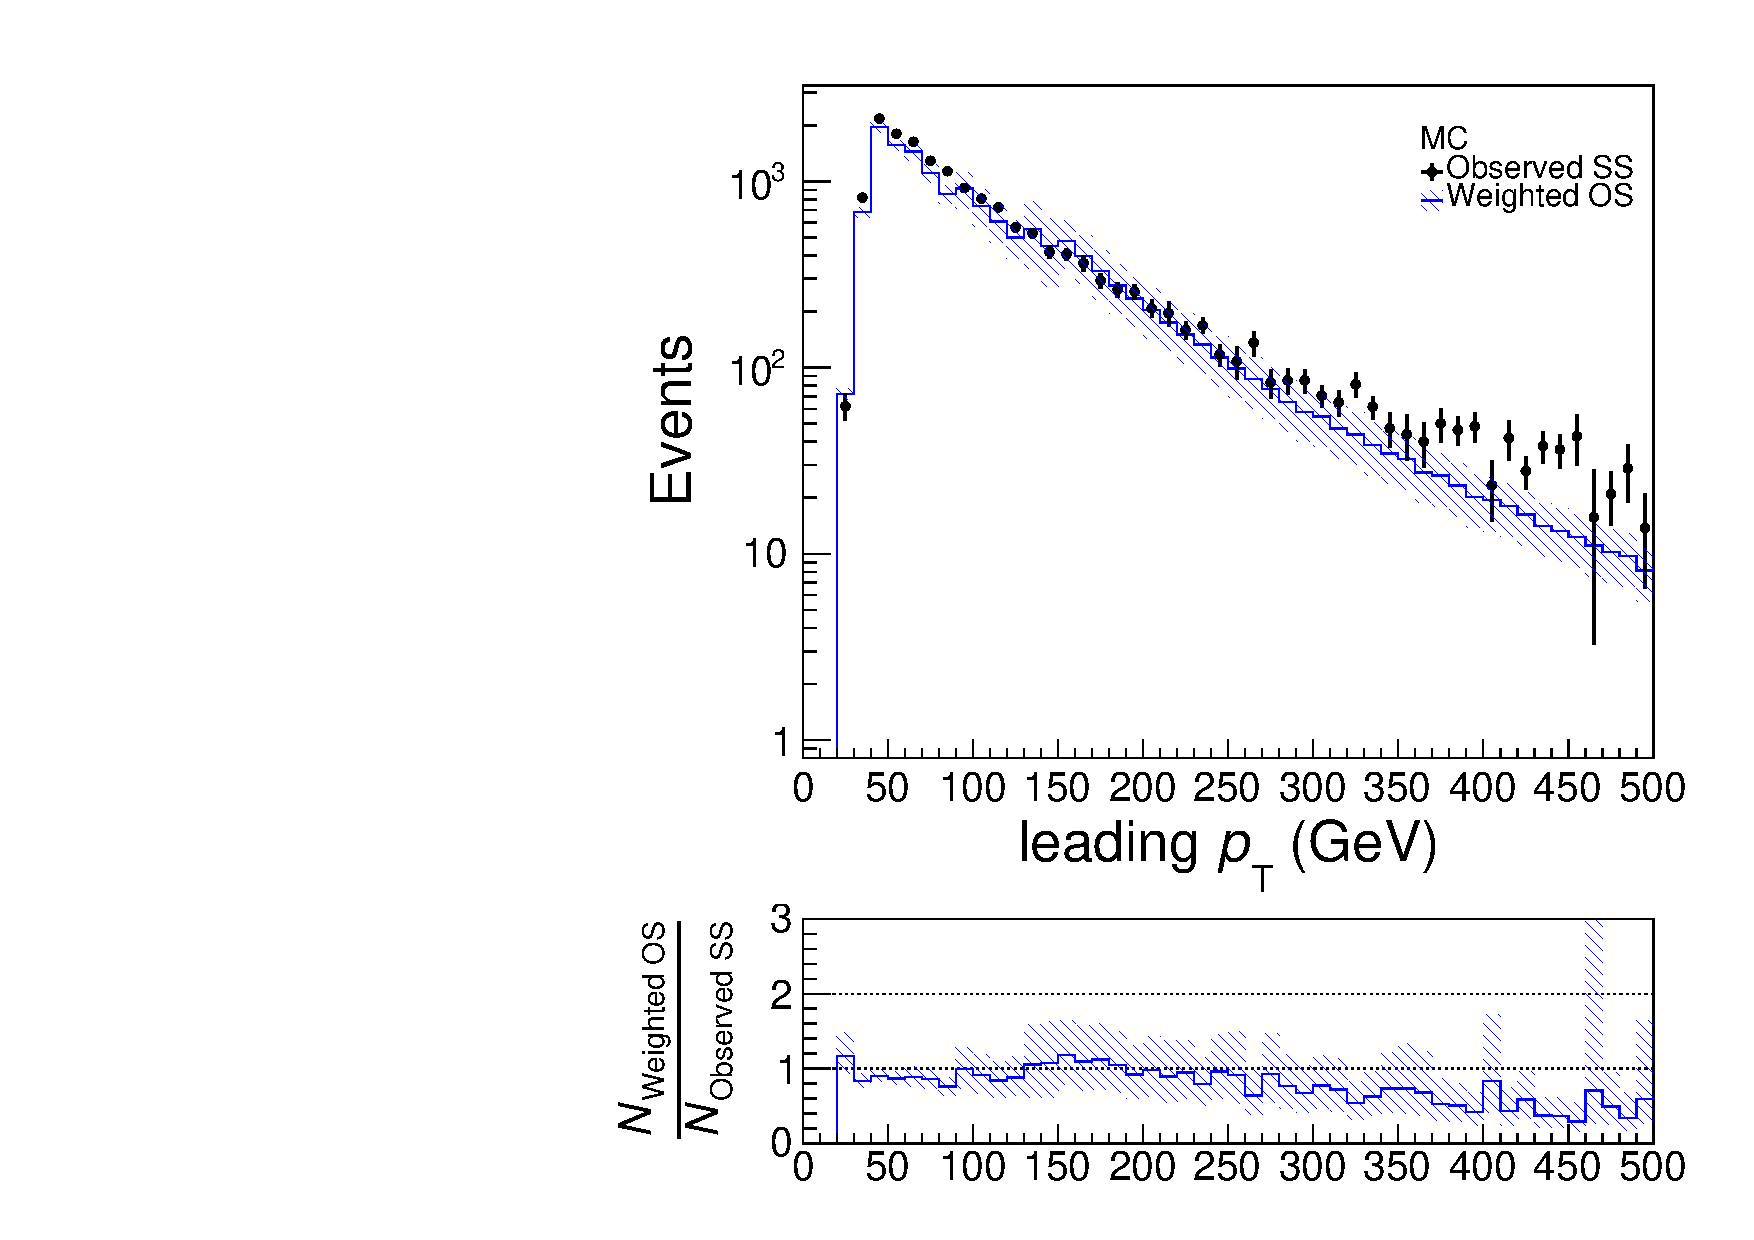
\includegraphics[width=0.3\textwidth]{data/plot/charge_flip/ReweightPlots/plots_NOchfSF/mc_pt_1.pdf}
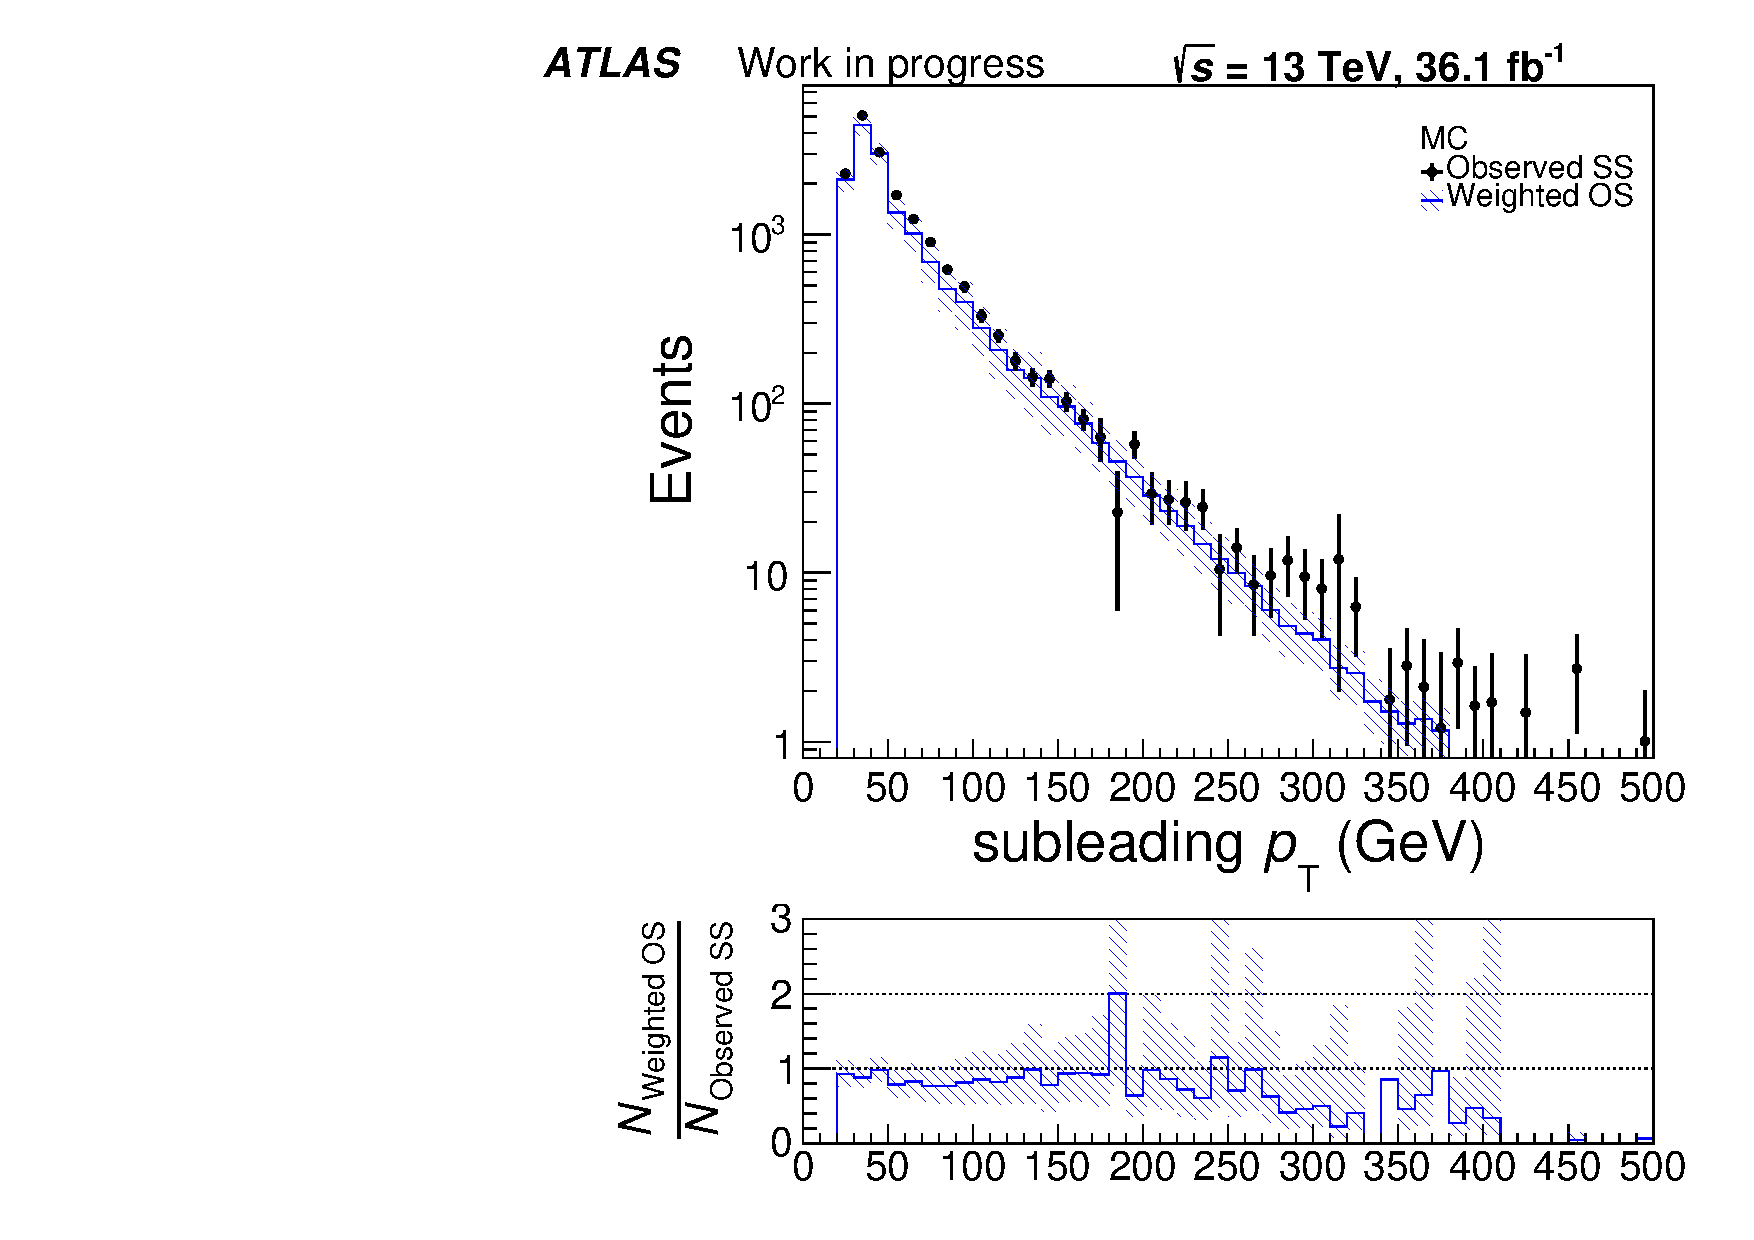
\includegraphics[width=0.3\textwidth]{data/plot/charge_flip/ReweightPlots/plots_NOchfSF/mc_pt_2.pdf} \\
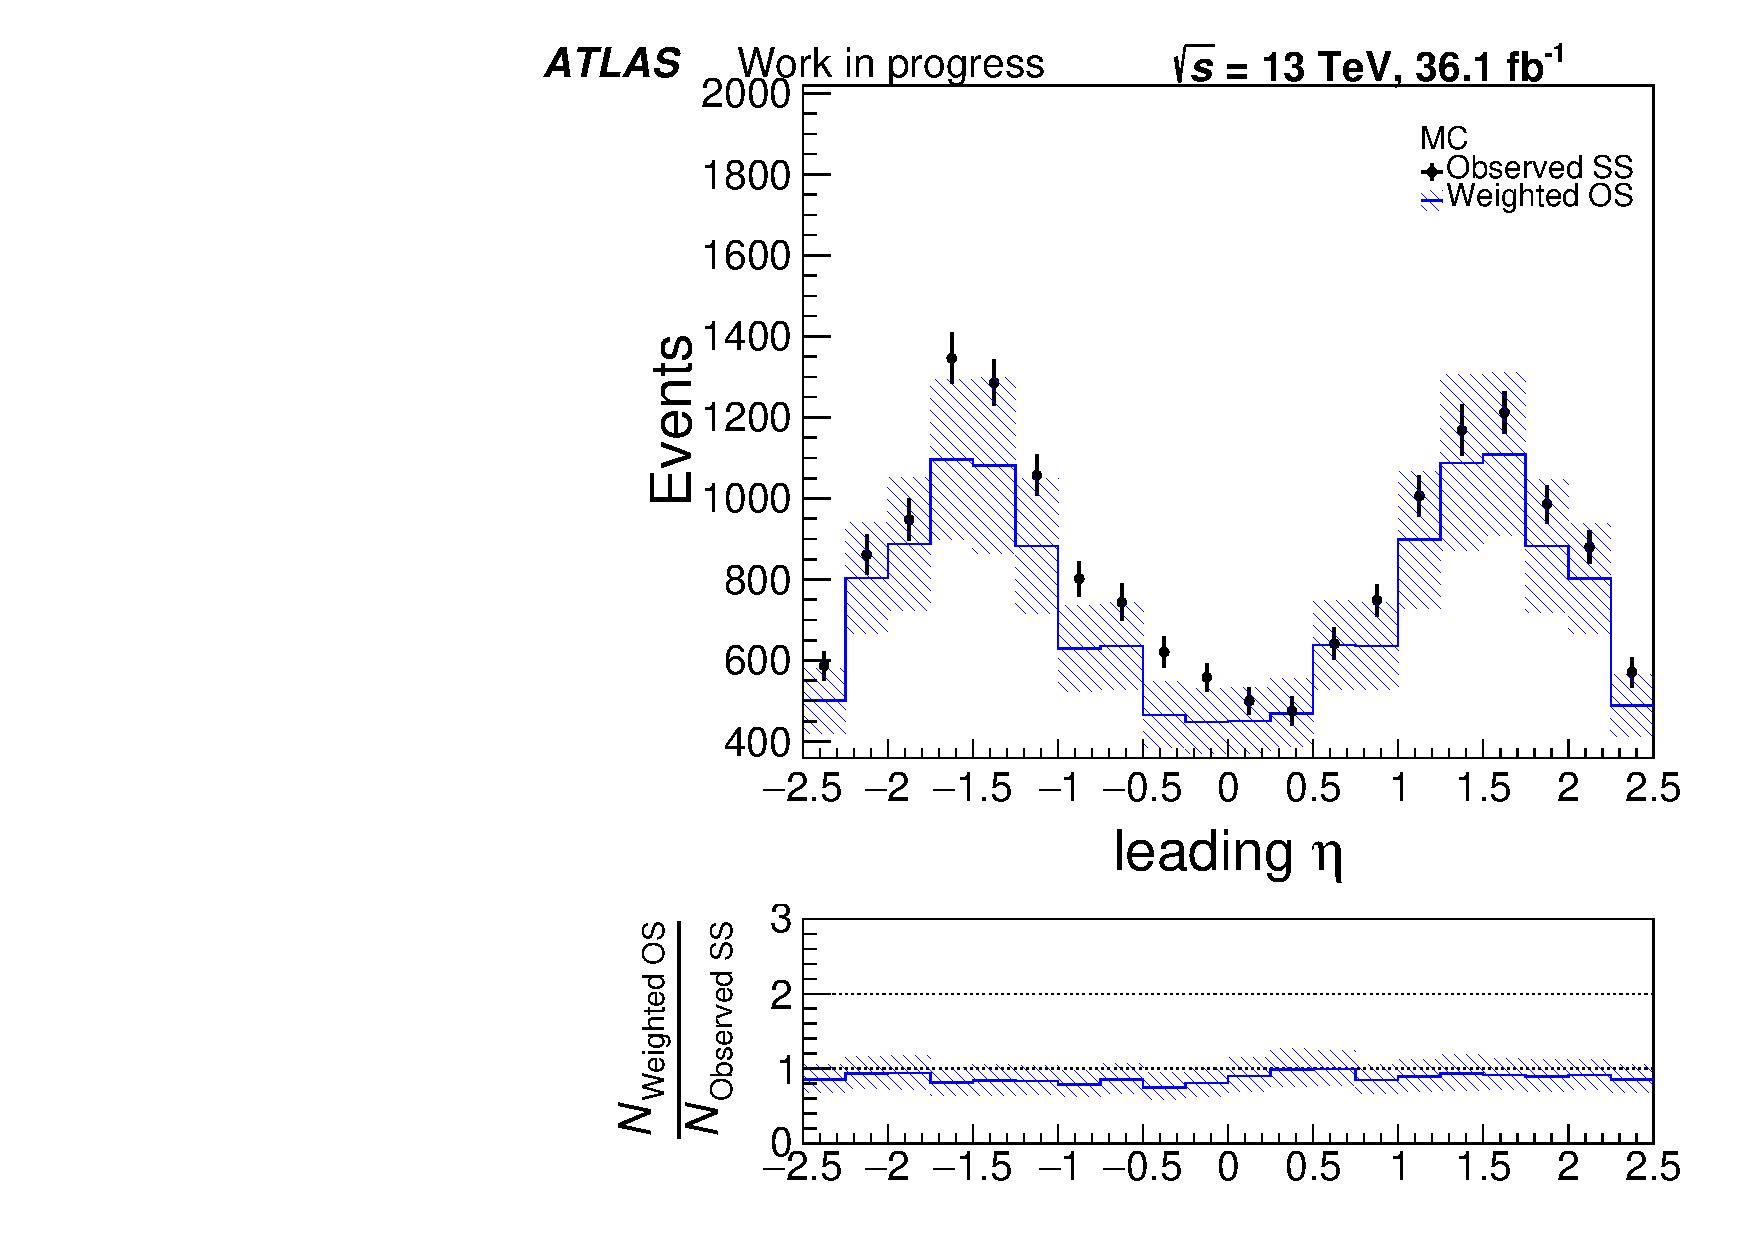
\includegraphics[width=0.3\textwidth]{data/plot/charge_flip/ReweightPlots/plots_NOchfSF/mc_eta_1.pdf}
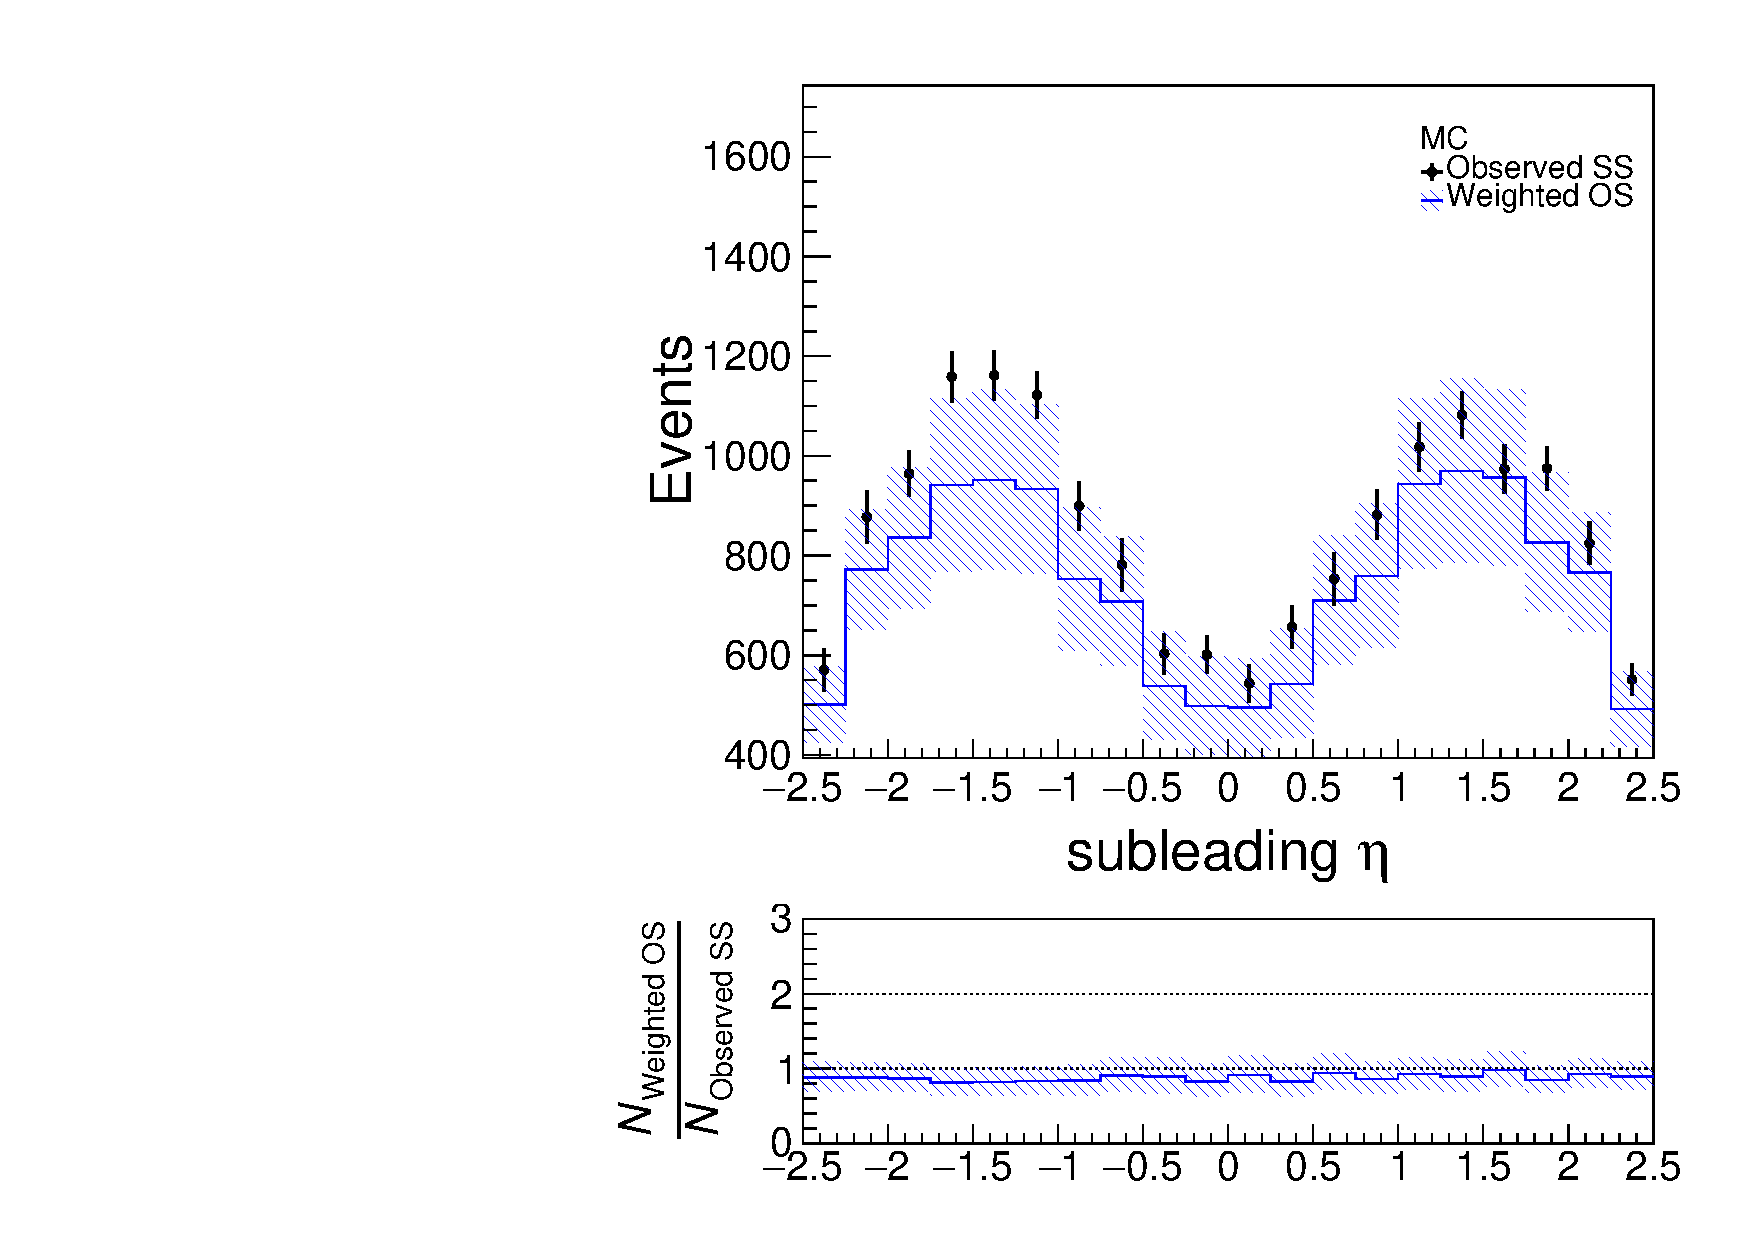
\includegraphics[width=0.3\textwidth]{data/plot/charge_flip/ReweightPlots/plots_NOchfSF/mc_eta_2.pdf} \\
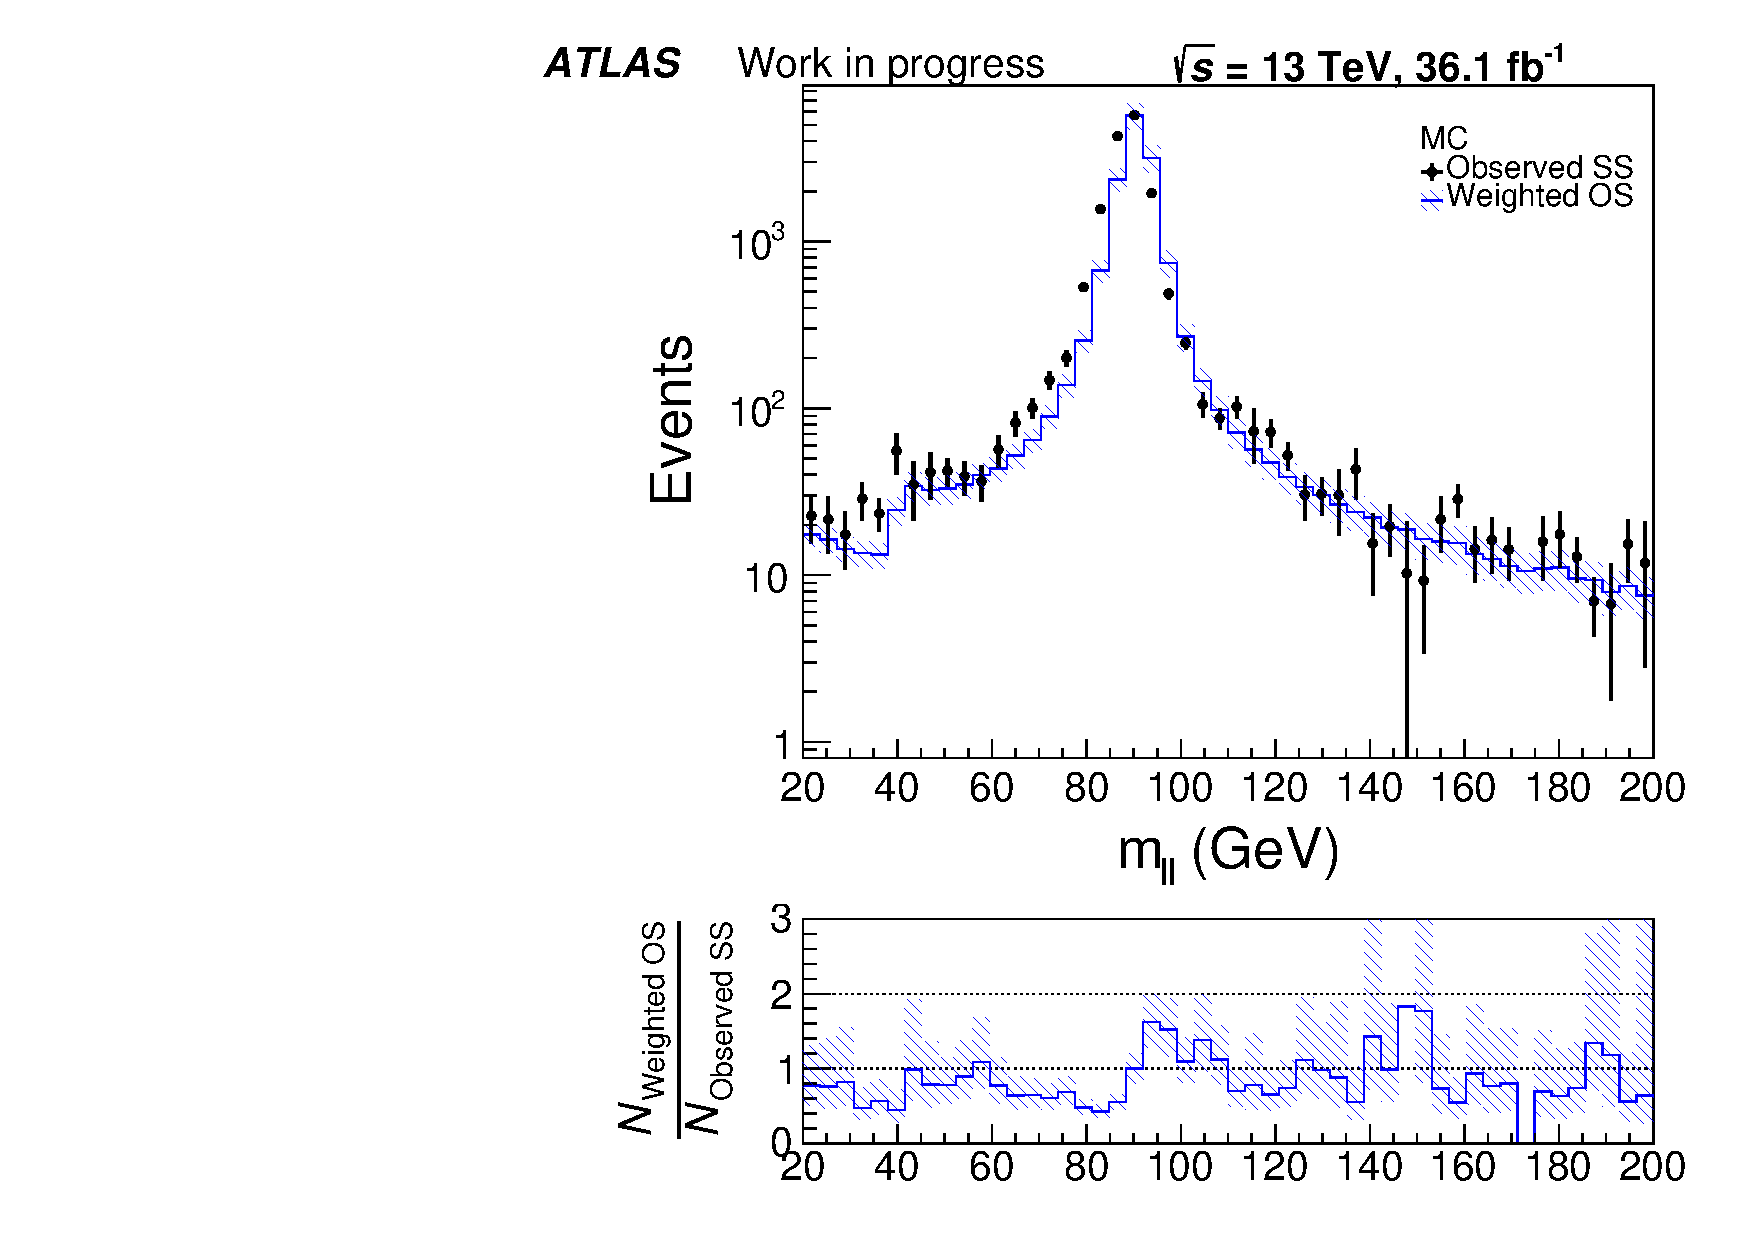
\includegraphics[width=0.3\textwidth]{data/plot/charge_flip/ReweightPlots/plots_NOchfSF/mc_mll.pdf}
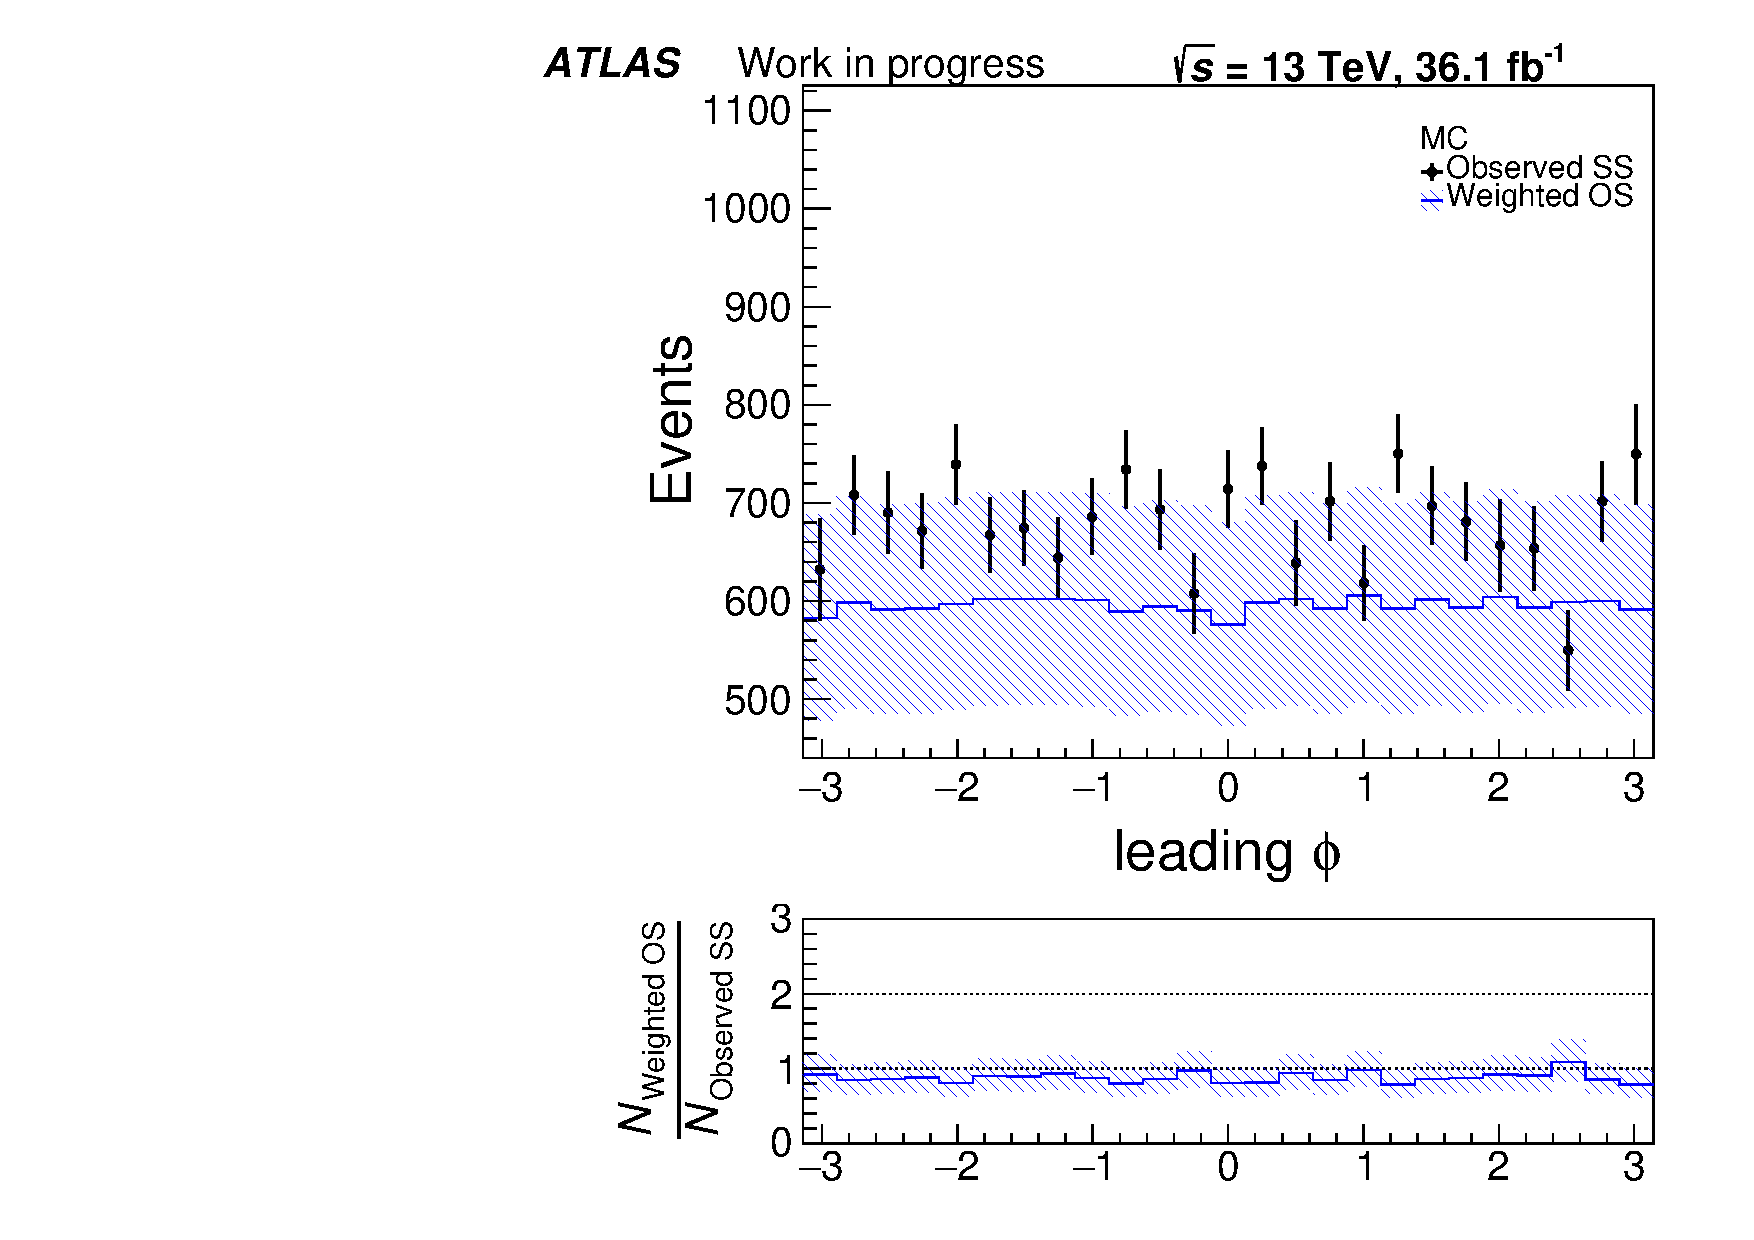
\includegraphics[width=0.3\textwidth]{data/plot/charge_flip/ReweightPlots/plots_NOchfSF/mc_phi_1.pdf}
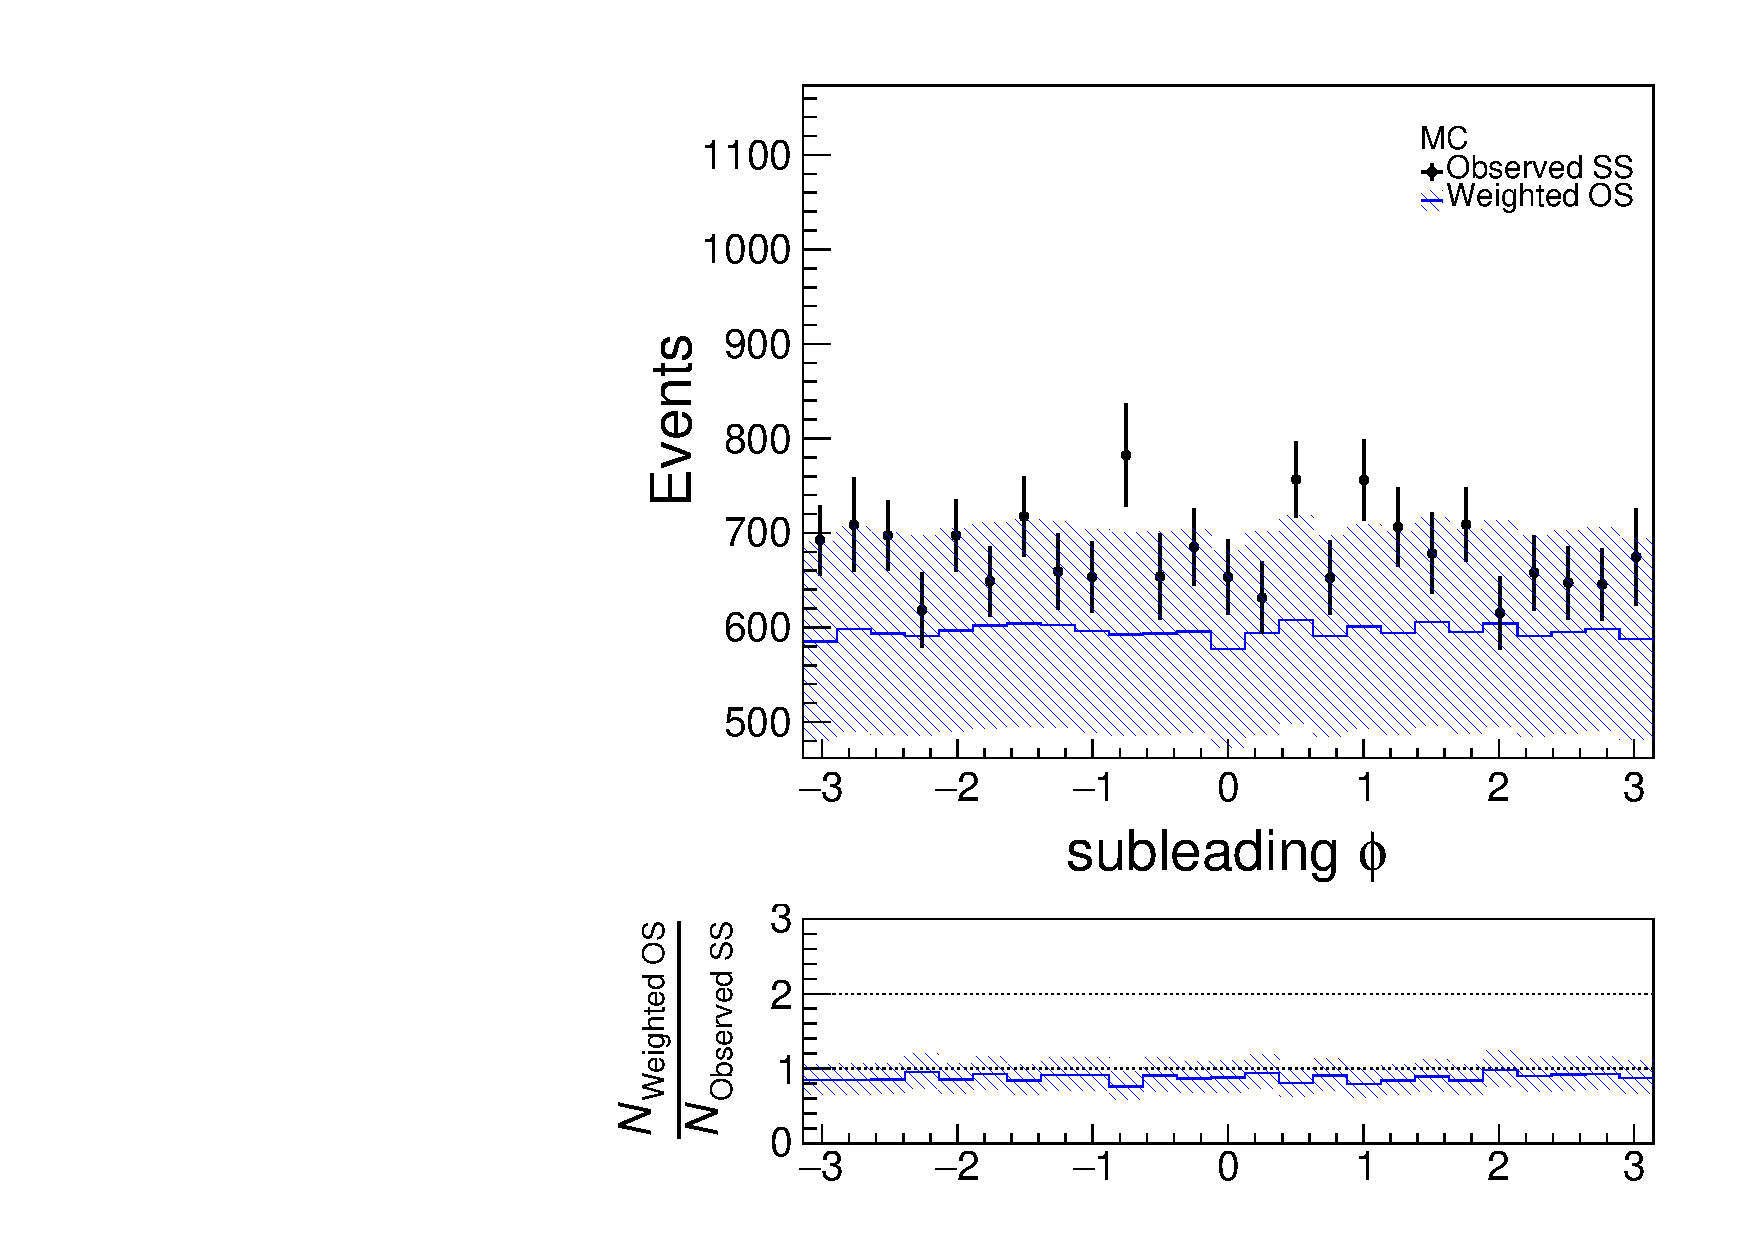
\includegraphics[width=0.3\textwidth]{data/plot/charge_flip/ReweightPlots/plots_NOchfSF/mc_phi_2.pdf}
\caption{The comparisons between the weighted OS events and the SS events.}
\label{fig:charge_flip_MC_validation}
\end{figure}

\section{Fake lepton background}
\label{sec:fake_background}
\subsection{Sources for fake lepton background}
The fake lepton background is ascribed to the case that other particles like meson, hadron and photon are misidentified as leptons.
Three types of fake lepton background are described as follows.
\begin{itemize}
\item Heavy-flavor fakes:
\begin{itemize}
\item It comes from semi-leptonic decays of heavy-quark (b or c) hadrons in jets
\end{itemize}
\item Light-flavor fakes:
\begin{itemize}
\item It comes from semi-leptonic decays of light-quark hadrons in jets
\item or comes from mis-reconstructions of jets from light-quark hadrons
\end{itemize}
\item photon conversion:
\begin{itemize}
\item It comes from the pair production from a photon
\end{itemize}
\end{itemize}
These leptons do not often pass the lepton identification cuts and have large impact parameters.

\subsection{Matrix method}
The fake lepton background is estimated with the matrix method.
The input of this method is the real and fake efficiencies of electron and muon, in different bins of $p_T$ and $|\eta|$, which are measured in the sections \ref{sec:real_eff} and \ref{sec:fake_eff}.
This method will estimate the amount of fake lepton background, by counting the number of loose and tight leptons in data.
The tight leptons in our analysis are the signal leptons, and the loose leptons are baseline leptons but not signal leptons.

The probability that a real electron (or muon) passes the signal selection (i.e. tight lepton) is denoted by the real efficiency $\epsilon$.
The probability that a real electron (or muon) does not pass the signal selection (i.e. loose lepton) is denoted by $\bar{\epsilon} = 1 - \epsilon$.
Similarly, the probability that a fake electron (or muon) passes the signal selection (i.e. tight lepton) is denoted by the fake efficiency $f$.
The probability that a fake electron (or muon) does not pass the signal selection (i.e. loose lepton) is denoted by $\bar{f} = 1 - f$.
Although there are no subscripts and superscripts for the efficiencies $e$ and $f$, these efficiencies are different for different flavours of the leptons (electron or muon), and depend on $p_T$ and $|\eta|$.

For simplicity, we first consider the case with only one lepton. We will then generalize to the case with two leptons.
By the definition of the efficiencies, the relation between the number of real/fake leptons and the number of tight/loose leptons is given by the following matrix.
\begin{equation}
\left( \begin{array}{c}
N_T \\
N_L
\end{array} \right)
=
\left( \begin{array}{cc}
\epsilon & f \\
\bar{\epsilon} & \bar{f}
\end{array} \right)
\left( \begin{array}{c}
N_R \\
N_F
\end{array} \right)
\label{equ:fake_eff_def}
\end{equation}
Because the number of tight/loose leptons can be counted in data, $\left( \begin{array}{c}
N_T \\
N_L
\end{array} \right)$ is known.
By inverting the matrix, the original number of fake leptons can be calculated.
\begin{align}
\begin{split}
\left( \begin{array}{c}
0 \\
N_F
\end{array} \right)
&=
\left( \begin{array}{cc}
0 & 0 \\
0 & 1
\end{array} \right)
\left( \begin{array}{c}
N_R \\
N_F
\end{array} \right) \\
&=
\left( \begin{array}{cc}
0 & 0 \\
0 & 1
\end{array} \right)
\left( \begin{array}{cc}
\epsilon & f \\
\bar{\epsilon} & \bar{f}
\end{array} \right)^{-1}
\left( \begin{array}{c}
N_T \\
N_L
\end{array} \right)
\end{split}
\end{align}
The fake lepton background, which is the number of tight lepton due to the fake lepton, $N_T'$, can then be found, by re-apply the matrix in equation \ref{equ:fake_eff_def}.
\begin{align}
\begin{split}
\left( \begin{array}{c}
N_T' \\
N_L'
\end{array} \right)
&=
\left( \begin{array}{cc}
\epsilon & f \\
\bar{\epsilon} & \bar{f}
\end{array} \right)
\left( \begin{array}{c}
0 \\
N_F
\end{array} \right) \\
&=
\left( \begin{array}{cc}
\epsilon & f \\
\bar{\epsilon} & \bar{f}
\end{array} \right)
\left( \begin{array}{cc}
0 & 0 \\
0 & 1
\end{array} \right)
\left( \begin{array}{cc}
\epsilon & f \\
\bar{\epsilon} & \bar{f}
\end{array} \right)^{-1}
\left( \begin{array}{c}
N_T \\
N_L
\end{array} \right) \\
N_T'
&=
\left( \begin{array}{cc}
\epsilon & f \\
\end{array} \right)
\left( \begin{array}{cc}
0 & 0 \\
0 & 1
\end{array} \right)
\left( \begin{array}{cc}
\epsilon & f \\
\bar{\epsilon} & \bar{f}
\end{array} \right)^{-1}
\left( \begin{array}{c}
N_T \\
N_L
\end{array} \right) \\
\end{split}
\end{align}

To generalize to the case with two leptons, equation \ref{equ:fake_eff_def} becomes
\begin{equation}
\left( \begin{array}{c}
N_{TT} \\
N_{TL} \\
N_{LT} \\
N_{LL}
\end{array} \right)
=
\left( \begin{array}{cccc}
\epsilon_1 \epsilon_2 & \epsilon_1 f_2 & f_1 \epsilon_2 & f_1 f_2 \\
\epsilon_1 \bar{\epsilon_2} & \epsilon_1 \bar{f_2} & f_1 \bar{\epsilon_2} & f_1 \bar{f_2} \\
\bar{\epsilon_1} \epsilon_2 & \bar{\epsilon_1} f_2 & \bar{f_1} \epsilon_2 & \bar{f_1} f_2 \\
\bar{\epsilon_1} \bar{\epsilon_2} & \bar{\epsilon_1} \bar{f_2} & \bar{f_1} \bar{\epsilon_2} & \bar{f_1} \bar{f_2}
\end{array} \right)
\left( \begin{array}{c}
N_{RR} \\
N_{RF} \\
N_{FR} \\
N_{FF}
\end{array} \right)
\end{equation}
where the subscripts 1 and 2 of the efficiencies denote the leading lepton and sub-leading lepton respectively.
The two letters in the subscript of $N$ describe the types of the leading and sub-leading lepton respectively.
$N_{RF}$, $N_{FR}$, $N_{FF}$ can be found by inverting the matrix.
\begin{align}
\begin{split}
\left( \begin{array}{c}
0 \\
N_{RF} \\
N_{FR} \\
N_{FF}
\end{array} \right)
&=
\left( \begin{array}{cccc}
0 & 0 & 0 & 0 \\
0 & 1 & 0 & 0 \\
0 & 0 & 1 & 0 \\
0 & 0 & 0 & 1
\end{array} \right)
\left( \begin{array}{c}
N_{RR} \\
N_{RF} \\
N_{FR} \\
N_{FF}
\end{array} \right) \\
&=
\left( \begin{array}{cccc}
0 & 0 & 0 & 0 \\
0 & 1 & 0 & 0 \\
0 & 0 & 1 & 0 \\
0 & 0 & 0 & 1
\end{array} \right)
\left( \begin{array}{cccc}
\epsilon_1 \epsilon_2 & \epsilon_1 f_2 & f_1 \epsilon_2 & f_1 f_2 \\
\epsilon_1 \bar{\epsilon_2} & \epsilon_1 \bar{f_2} & f_1 \bar{\epsilon_2} & f_1 \bar{f_2} \\
\bar{\epsilon_1} \epsilon_2 & \bar{\epsilon_1} f_2 & \bar{f_1} \epsilon_2 & \bar{f_1} f_2 \\
\bar{\epsilon_1} \bar{\epsilon_2} & \bar{\epsilon_1} \bar{f_2} & \bar{f_1} \bar{\epsilon_2} & \bar{f_1} \bar{f_2}
\end{array} \right)^{-1}
\left( \begin{array}{c}
N_{TT} \\
N_{TL} \\
N_{LT} \\
N_{LL}
\end{array} \right)
\end{split}
\end{align}
The fake lepton background, which is the number of tight-tight lepton due to the fake lepton, $N_{TT}'$, can then be found.
\begin{align}
\begin{split}
\left( \begin{array}{c}
N_{TT}' \\
N_{TL}' \\
N_{LT}' \\
N_{LL}'
\end{array} \right)
&=
\left( \begin{array}{cccc}
\epsilon_1 \epsilon_2 & \epsilon_1 f_2 & f_1 \epsilon_2 & f_1 f_2 \\
\epsilon_1 \bar{\epsilon_2} & \epsilon_1 \bar{f_2} & f_1 \bar{\epsilon_2} & f_1 \bar{f_2} \\
\bar{\epsilon_1} \epsilon_2 & \bar{\epsilon_1} f_2 & \bar{f_1} \epsilon_2 & \bar{f_1} f_2 \\
\bar{\epsilon_1} \bar{\epsilon_2} & \bar{\epsilon_1} \bar{f_2} & \bar{f_1} \bar{\epsilon_2} & \bar{f_1} \bar{f_2}
\end{array} \right)
\left( \begin{array}{c}
0 \\
N_{RF} \\
N_{FR} \\
N_{FF}
\end{array} \right) \\
&=
\left( \begin{array}{cccc}
\epsilon_1 \epsilon_2 & \epsilon_1 f_2 & f_1 \epsilon_2 & f_1 f_2 \\
\epsilon_1 \bar{\epsilon_2} & \epsilon_1 \bar{f_2} & f_1 \bar{\epsilon_2} & f_1 \bar{f_2} \\
\bar{\epsilon_1} \epsilon_2 & \bar{\epsilon_1} f_2 & \bar{f_1} \epsilon_2 & \bar{f_1} f_2 \\
\bar{\epsilon_1} \bar{\epsilon_2} & \bar{\epsilon_1} \bar{f_2} & \bar{f_1} \bar{\epsilon_2} & \bar{f_1} \bar{f_2}
\end{array} \right)
\left( \begin{array}{cccc}
0 & 0 & 0 & 0 \\
0 & 1 & 0 & 0 \\
0 & 0 & 1 & 0 \\
0 & 0 & 0 & 1
\end{array} \right)
\left( \begin{array}{cccc}
\epsilon_1 \epsilon_2 & \epsilon_1 f_2 & f_1 \epsilon_2 & f_1 f_2 \\
\epsilon_1 \bar{\epsilon_2} & \epsilon_1 \bar{f_2} & f_1 \bar{\epsilon_2} & f_1 \bar{f_2} \\
\bar{\epsilon_1} \epsilon_2 & \bar{\epsilon_1} f_2 & \bar{f_1} \epsilon_2 & \bar{f_1} f_2 \\
\bar{\epsilon_1} \bar{\epsilon_2} & \bar{\epsilon_1} \bar{f_2} & \bar{f_1} \bar{\epsilon_2} & \bar{f_1} \bar{f_2}
\end{array} \right)^{-1}
\left( \begin{array}{c}
N_{TT} \\
N_{TL} \\
N_{LT} \\
N_{LL}
\end{array} \right) \\
N_{TT}'
&=
\left( \begin{array}{cccc}
\epsilon_1 \epsilon_2 & \epsilon_1 f_2 & f_1 \epsilon_2 & f_1 f_2 \\
\end{array} \right)
\left( \begin{array}{cccc}
0 & 0 & 0 & 0 \\
0 & 1 & 0 & 0 \\
0 & 0 & 1 & 0 \\
0 & 0 & 0 & 1
\end{array} \right)
\left( \begin{array}{cccc}
\epsilon_1 \epsilon_2 & \epsilon_1 f_2 & f_1 \epsilon_2 & f_1 f_2 \\
\epsilon_1 \bar{\epsilon_2} & \epsilon_1 \bar{f_2} & f_1 \bar{\epsilon_2} & f_1 \bar{f_2} \\
\bar{\epsilon_1} \epsilon_2 & \bar{\epsilon_1} f_2 & \bar{f_1} \epsilon_2 & \bar{f_1} f_2 \\
\bar{\epsilon_1} \bar{\epsilon_2} & \bar{\epsilon_1} \bar{f_2} & \bar{f_1} \bar{\epsilon_2} & \bar{f_1} \bar{f_2}
\end{array} \right)^{-1}
\left( \begin{array}{c}
N_{TT} \\
N_{TL} \\
N_{LT} \\
N_{LL}
\end{array} \right)
\end{split}
\label{equ:fake_eff_matrix}
\end{align}
Equation \ref{equ:fake_eff_matrix} can be applied to any combination of the flavours, $p_T$ and $|\eta|$ of the leading and sub-leading lepton.
In principle, the total amount of fake lepton background should be the summation of all combinations of the flavours, $p_T$ and $|\eta|$.
For a particular combination, the counting result of the tight/loose leptons in data $\left( \begin{array}{c}
N_{TT} \\
N_{TL} \\
N_{LT} \\
N_{LL}
\end{array} \right)$ can be split into ``one'', which is the contribution by one event:
\begin{align}
\begin{split}
\left( \begin{array}{c}
N_{TT} \\
N_{TL} \\
N_{LT} \\
N_{LL}
\end{array} \right)
=
\sum_{i=1}^{N_{TT}}
\left( \begin{array}{c}
1 \\
0 \\
0 \\
0
\end{array} \right)
+
\sum_{i=1}^{N_{TL}}
\left( \begin{array}{c}
0 \\
1 \\
0 \\
0
\end{array} \right)
+
\sum_{i=1}^{N_{LT}}
\left( \begin{array}{c}
0 \\
0 \\
1 \\
0
\end{array} \right)
+
\sum_{i=1}^{N_{LL}}
\left( \begin{array}{c}
0 \\
0 \\
0 \\
1
\end{array} \right)
\end{split}
\end{align}
Because equation \ref{equ:fake_eff_matrix} is a linear function, we can first calculate the small contribution of $N_{TT}'$ from one event, and assign this value as a weight to the event.
This weight is called the fake weight of the event.
The total fake lepton background is then the sum of the fake weight of all events in data.
For example, if a pair of two leptons is a tight-tight pair, the fake weight of this event is $N_{TT}'$ in the following equation.
\begin{align}
\begin{split}
N_{TT}'
=
\left( \begin{array}{cccc}
\epsilon_1 \epsilon_2 & \epsilon_1 f_2 & f_1 \epsilon_2 & f_1 f_2 \\
\end{array} \right)
\left( \begin{array}{cccc}
0 & 0 & 0 & 0 \\
0 & 1 & 0 & 0 \\
0 & 0 & 1 & 0 \\
0 & 0 & 0 & 1
\end{array} \right)
\left( \begin{array}{cccc}
\epsilon_1 \epsilon_2 & \epsilon_1 f_2 & f_1 \epsilon_2 & f_1 f_2 \\
\epsilon_1 \bar{\epsilon_2} & \epsilon_1 \bar{f_2} & f_1 \bar{\epsilon_2} & f_1 \bar{f_2} \\
\bar{\epsilon_1} \epsilon_2 & \bar{\epsilon_1} f_2 & \bar{f_1} \epsilon_2 & \bar{f_1} f_2 \\
\bar{\epsilon_1} \bar{\epsilon_2} & \bar{\epsilon_1} \bar{f_2} & \bar{f_1} \bar{\epsilon_2} & \bar{f_1} \bar{f_2}
\end{array} \right)^{-1}
\left( \begin{array}{c}
1 \\
0 \\
0 \\
0
\end{array} \right)
\end{split}
\label{equ:fake_eff_fake_weight}
\end{align}
where the flavours, $p_T$ and $|\eta|$ of the efficiencies are simply the flavours, $p_T$ and $|\eta|$ of the leading and sub-leading lepton in this event.

By inversing the matrix, equation \ref{equ:fake_eff_matrix} can be simplified.
First, we define a variable $d$.
\begin{align}
\begin{split}
d = (\epsilon_1 - f_1) (\epsilon_2 - f_2)
\end{split}
\end{align}
The inverse of the matrix is given by
\begin{align}
\begin{split}
\left( \begin{array}{cccc}
\epsilon_1 \epsilon_2 & \epsilon_1 f_2 & f_1 \epsilon_2 & f_1 f_2 \\
\epsilon_1 \bar{\epsilon_2} & \epsilon_1 \bar{f_2} & f_1 \bar{\epsilon_2} & f_1 \bar{f_2} \\
\bar{\epsilon_1} \epsilon_2 & \bar{\epsilon_1} f_2 & \bar{f_1} \epsilon_2 & \bar{f_1} f_2 \\
\bar{\epsilon_1} \bar{\epsilon_2} & \bar{\epsilon_1} \bar{f_2} & \bar{f_1} \bar{\epsilon_2} & \bar{f_1} \bar{f_2}
\end{array} \right)^{-1}
= \frac{1}{d}
\left( \begin{array}{cccc}
  \bar{f_1}        \bar{f_2}        & - \bar{f_1}        f_2        & - f_1        \bar{f_2}        &   f_1        f_2        \\
- \bar{f_1}        \bar{\epsilon_2} &   \bar{f_1}        \epsilon_2 &   f_1        \bar{\epsilon_2} & - f_1        \epsilon_2 \\
- \bar{\epsilon_1} \bar{f_2}        &   \bar{\epsilon_1} f_2        &   \epsilon_1 \bar{f_2}        & - \epsilon_1 f_2        \\
  \bar{\epsilon_1} \bar{\epsilon_2} & - \bar{\epsilon_1} \epsilon_2 & - \epsilon_1 \bar{\epsilon_2} &   \epsilon_1 \epsilon_2 \\
\end{array} \right)
\end{split}
\end{align}
Equation \ref{equ:fake_eff_matrix} becomes
\begin{align}
\begin{split}
N_{TT}'
&=
\left( \begin{array}{cccc}
\epsilon_1 \epsilon_2 & \epsilon_1 f_2 & f_1 \epsilon_2 & f_1 f_2 \\
\end{array} \right)
\left( \begin{array}{cccc}
0 & 0 & 0 & 0 \\
0 & 1 & 0 & 0 \\
0 & 0 & 1 & 0 \\
0 & 0 & 0 & 1
\end{array} \right)
\frac{1}{d}
\left( \begin{array}{cccc}
  \bar{f_1}        \bar{f_2}        & - \bar{f_1}        f_2        & - f_1        \bar{f_2}        &   f_1        f_2        \\
- \bar{f_1}        \bar{\epsilon_2} &   \bar{f_1}        \epsilon_2 &   f_1        \bar{\epsilon_2} & - f_1        \epsilon_2 \\
- \bar{\epsilon_1} \bar{f_2}        &   \bar{\epsilon_1} f_2        &   \epsilon_1 \bar{f_2}        & - \epsilon_1 f_2        \\
  \bar{\epsilon_1} \bar{\epsilon_2} & - \bar{\epsilon_1} \epsilon_2 & - \epsilon_1 \bar{\epsilon_2} &   \epsilon_1 \epsilon_2 \\
\end{array} \right)
\left( \begin{array}{c}
N_{TT} \\
N_{TL} \\
N_{LT} \\
N_{LL}
\end{array} \right) \\
&=
\frac{1}{d}
\left( \begin{array}{cccc}
\epsilon_1 \epsilon_2 & \epsilon_1 f_2 & f_1 \epsilon_2 & f_1 f_2 \\
\end{array} \right)
\left( \begin{array}{cccc}
  0                                 &   0                           &   0                           &   0                     \\
- \bar{f_1}        \bar{\epsilon_2} &   \bar{f_1}        \epsilon_2 &   f_1        \bar{\epsilon_2} & - f_1        \epsilon_2 \\
- \bar{\epsilon_1} \bar{f_2}        &   \bar{\epsilon_1} f_2        &   \epsilon_1 \bar{f_2}        & - \epsilon_1 f_2        \\
  \bar{\epsilon_1} \bar{\epsilon_2} & - \bar{\epsilon_1} \epsilon_2 & - \epsilon_1 \bar{\epsilon_2} &   \epsilon_1 \epsilon_2 \\
\end{array} \right)
\left( \begin{array}{c}
N_{TT} \\
N_{TL} \\
N_{LT} \\
N_{LL}
\end{array} \right) \\
\end{split}
\end{align}
For a tight-tight pair,
\begin{align}
\begin{split}
\text{fake weight} = \frac{1}{d} (
- \epsilon_1 \bar{f_1} \bar{\epsilon_2} f_2
- \bar{\epsilon_1} f_1 \epsilon_2 \bar{f_2}
+ \bar{\epsilon_1} f_1 \bar{\epsilon_2} f_2 )
\end{split}
\end{align}
For a tight-loose pair,
\begin{align}
\begin{split}
\text{fake weight} &= \frac{1}{d} (
\epsilon_1 \bar{f_1} \epsilon_2 f_2
+ \bar{\epsilon_1} f_1 \epsilon_2 f_2
- \bar{\epsilon_1} f_1 \epsilon_2 f_2 ) \\
&= \frac{\epsilon_1 \bar{f_1} \epsilon_2 f_2}{d}
\end{split}
\end{align}
For a loose-tight pair,
\begin{align}
\begin{split}
\text{fake weight} &= \frac{1}{d} (
\epsilon_1 f_1 \bar{\epsilon_2} f_2
+ \epsilon_1 f_1 \epsilon_2 \bar{f_2}
- \epsilon_1 f_1 \bar{\epsilon_2} f_2 ) \\
&= \frac{\epsilon_1 f_1 \epsilon_2 \bar{f_2}}{d}
\end{split}
\end{align}
For a loose-loose pair,
\begin{align}
\begin{split}
\text{fake weight} &= \frac{1}{d} (
- \epsilon_1 f_1 \epsilon_2 f_2
- \epsilon_1 f_1 \epsilon_2 f_2
+ \epsilon_1 f_1 \epsilon_2 f_2 ) \\
&= - \frac{\epsilon_1 f_1 \epsilon_2 f_2}{d}
\end{split}
\end{align}

\subsection{Measurement of real efficiencies}
\label{sec:real_eff}
The real efficiencies $\epsilon_i$ are measured by the Z boson tag-and-probe method.
This method is based on the fact that the Z bosons decay into two opposite-sign electrons or two muons and the invariant mass of the two leptons is the mass of the Z boson (close to 91 GeV).
By selecting two opposite-sign same-flavour leptons with the invariant mass 80 GeV $< m_{ll} <$ 100 GeV, these two leptons are likely to be real leptons from a Z boson decay.
If one of the leptons is a signal lepton, called the tag lepton, another lepton called the probe lepton is very likely to be a real lepton.
By counting the total number of baseline leptons and signal leptons for the probe lepton, the real efficiencies $\epsilon$ can be measured.
The counting is done in the data sample, and hence this is a data-driven method.
\begin{align}
\epsilon = \frac{N^{\text{data}}_{\text{signal}}}{N^{\text{data}}_{\text{baseline}}}
\end{align}

The selections for the control region used in the measurement of real efficiencies is, on top of the selections in section \ref{event_cleaning}, as follows:
\begin{itemize}
\item The two leptons are two electrons or two muons.
\item The electric charges of the two leptons are opposite sign.
\item 80 GeV $< m_{ll} <$ 100 GeV
\end{itemize}

If the two leptons are both signal leptons, both leptons can be tag leptons to increase the statistics.

The binning for $p_T$ and $|\eta|$ is shown in table \ref{tab:binning_real_eff}.
\begin{table}[htbp]
\centering
\begin{tabular}{|c|c|}
\hline
Variable & Boundary of the bins \\
\hline
$p_T$ (GeV) &  25, 35, 45, 55, 65, 75, 85, 95 \\
\hline
$|\eta|$ (For electrons) & 0, 0.8, 1.37, 1.52, 2.47 \\
\hline
$|\eta|$ (For muons) & 0, 0.6, 1.2, 1.8, 2.4 \\
\hline
\end{tabular}
\caption{Binning in $p_T$ and $|\eta|$ for real efficiencies.}
\label{tab:binning_real_eff}
\end{table}

The results for the real efficiencies are shown in figure \ref{fig:result_real_eff}.
\begin{figure}[htpb]
\centering
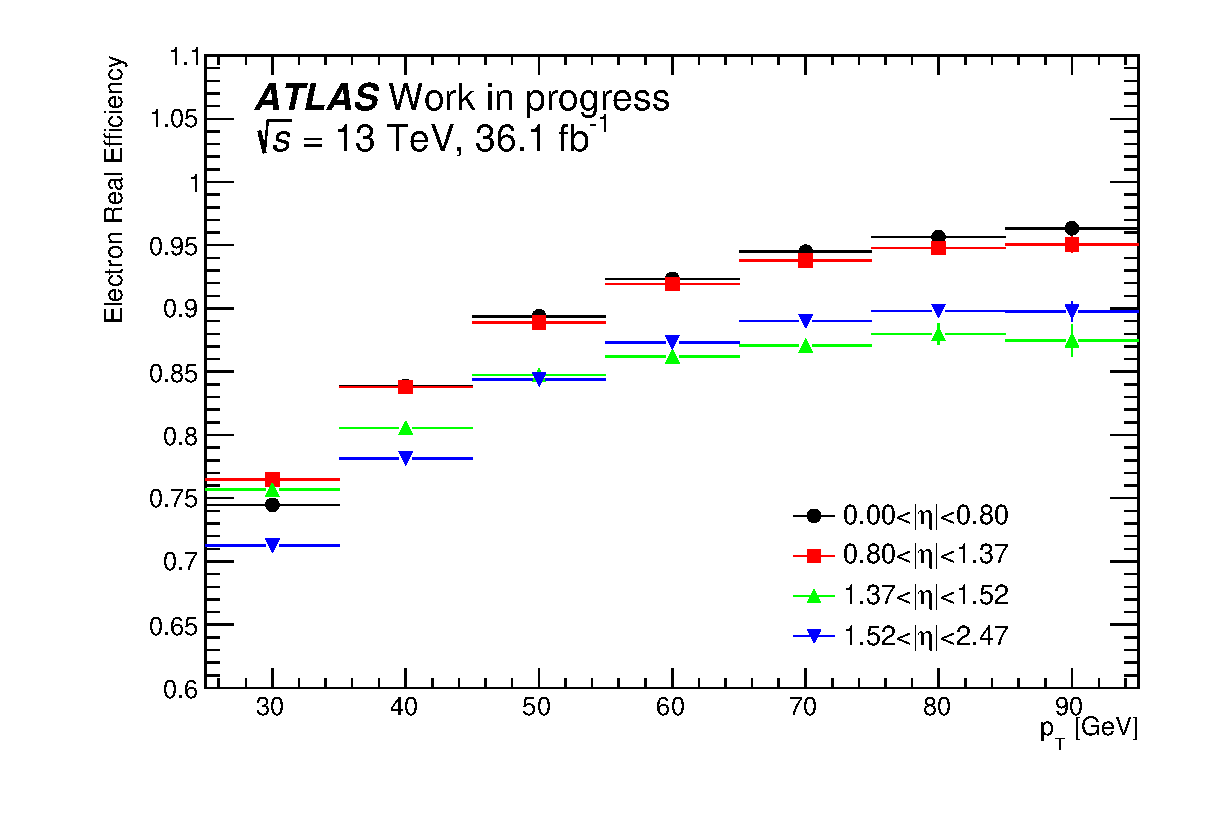
\includegraphics[width=0.49\linewidth]{data/plot/plotRealEffs/El_hEff.eps}
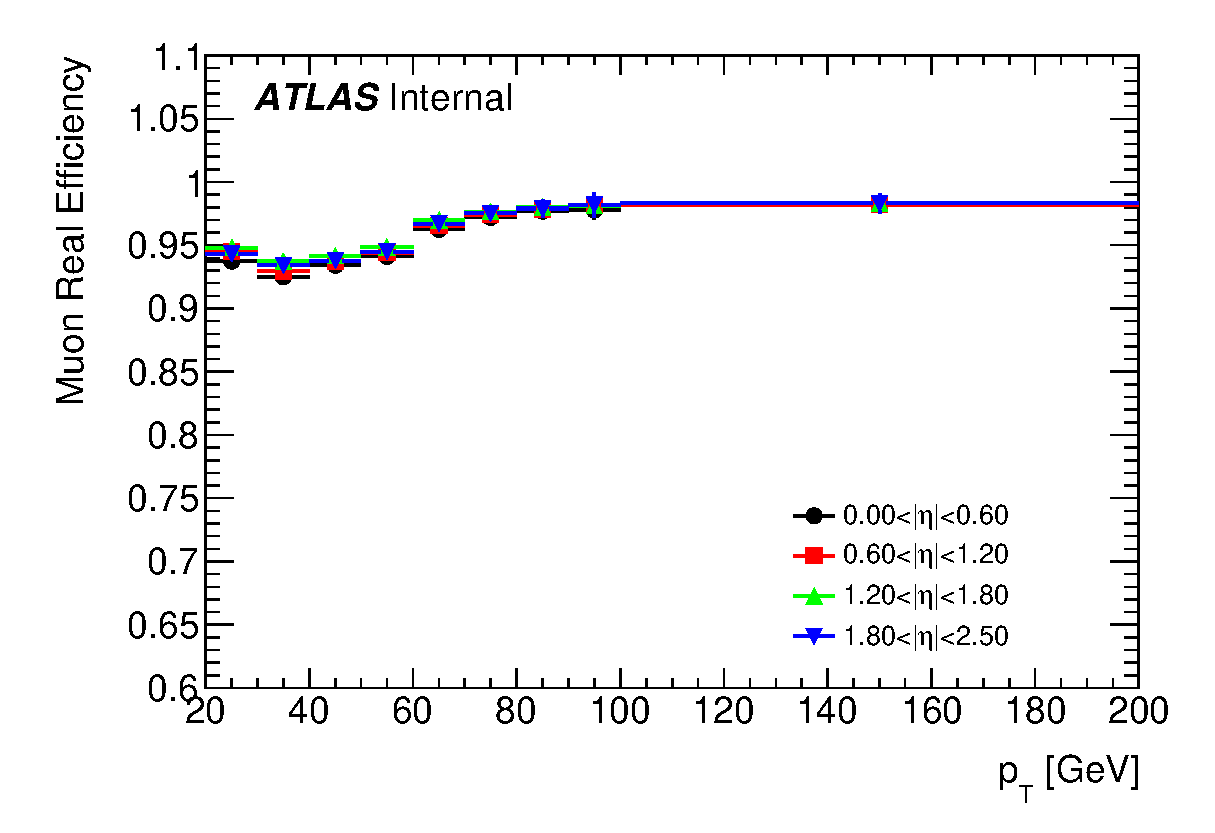
\includegraphics[width=0.49\linewidth]{data/plot/plotRealEffs/Mu_hEff.eps}
\caption{The real efficiencies for electrons (left) and muons (right). Only statistical uncertainties are considered.}
\label{fig:result_real_eff}
\end{figure}

\subsection{Measurement of fake efficiencies}
\label{sec:fake_eff}
The fake efficiencies are measured by the tag-and-probe method, similar to the real efficiencies.
On top of the selections in section \ref{event_cleaning}, two different control regions are defined for electron and muon respectively.
The control regions contain rich heavy-flavor fakes by requiring at least one b-jet.
The selections for the control regions are summarized as follows:
\begin{itemize}
\item For electron fake efficiencies, one lepton is a muon and another is an electron. For muons fake efficiencies, the two leptons are both muons.
\item The electric charges of the two leptons are same sign.
\item There is at least 1 b-jet.
\end{itemize}

In both control regions, the tag leptons must be a signal muon with $p_T > 40$ GeV.
The probe lepton is very likely to a fake lepton from heavy-flavor jets, because the two leptons are same-sign and the tag lepton is very likely to be a real lepton.
By counting the number of the baseline and signal probe leptons, the fake efficiencies can be estimated.
This counting is done in the data samples.
In order to ensure that the probe leptons are not coming from real leptons, the number of real leptons estimated by the MC sample is subtracted.
These MC samples include WZ, WW, ZZ, VVV, higgs, multi-top and ttV.
\begin{align}
f &= \frac{N_{\text{signal}}}{N_{\text{baseline}}} \\
&= \frac{N^{\text{data}}_{\text{signal}} - N^{\text{MC, real}}_{\text{signal}}}{N^{\text{data}}_{\text{baseline}} - N^{\text{MC, real}}_{\text{baseline}}}
\end{align}

The identification of the real leptons in the MC samples is using the truth information.
It classifies the reconstructed lepton into different types of truth particle.
The origin of the reconstructed lepton are known.

The binning for $p_T$ and $|\eta|$ is shown in table \ref{tab:binning_fake_eff}.
\begin{table}[htbp]
\centering
\begin{tabular}{|c|c|}
\hline
Variable & Boundary of the bins \\
\hline
\hline
& Electrons \\
\hline
$p_T$ (GeV) &  25, 35, 45, 120, 200 \\
\hline
$|\eta|$ & 0, 1.37, 1.52, 2.47 \\
\hline
\hline
& Muons \\
\hline
$p_T$ (GeV) &  25, 30, 45, 120, 200 \\
\hline
$|\eta|$ & 0, 1.37, 1.52, 2.4 \\
\hline
\end{tabular}
\caption{Binning in $p_T$ and $|\eta|$ for fake efficiencies.}
\label{tab:binning_fake_eff}
\end{table}

The results for the fake efficiencies are shown in figure \ref{fig:result_fake_eff}.
\begin{figure}[htpb]
\centering
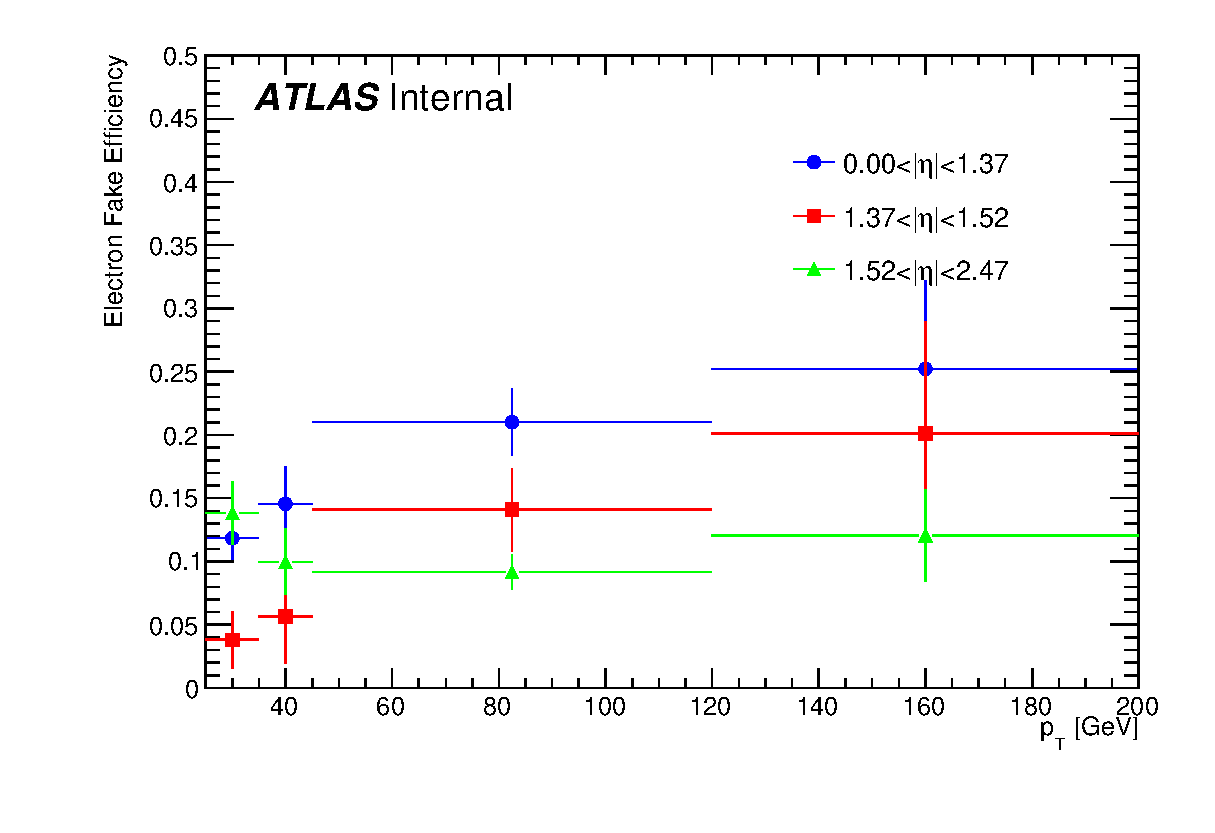
\includegraphics[width=0.49\linewidth]{data/plot/getFakeEffs/El_hEff.eps}
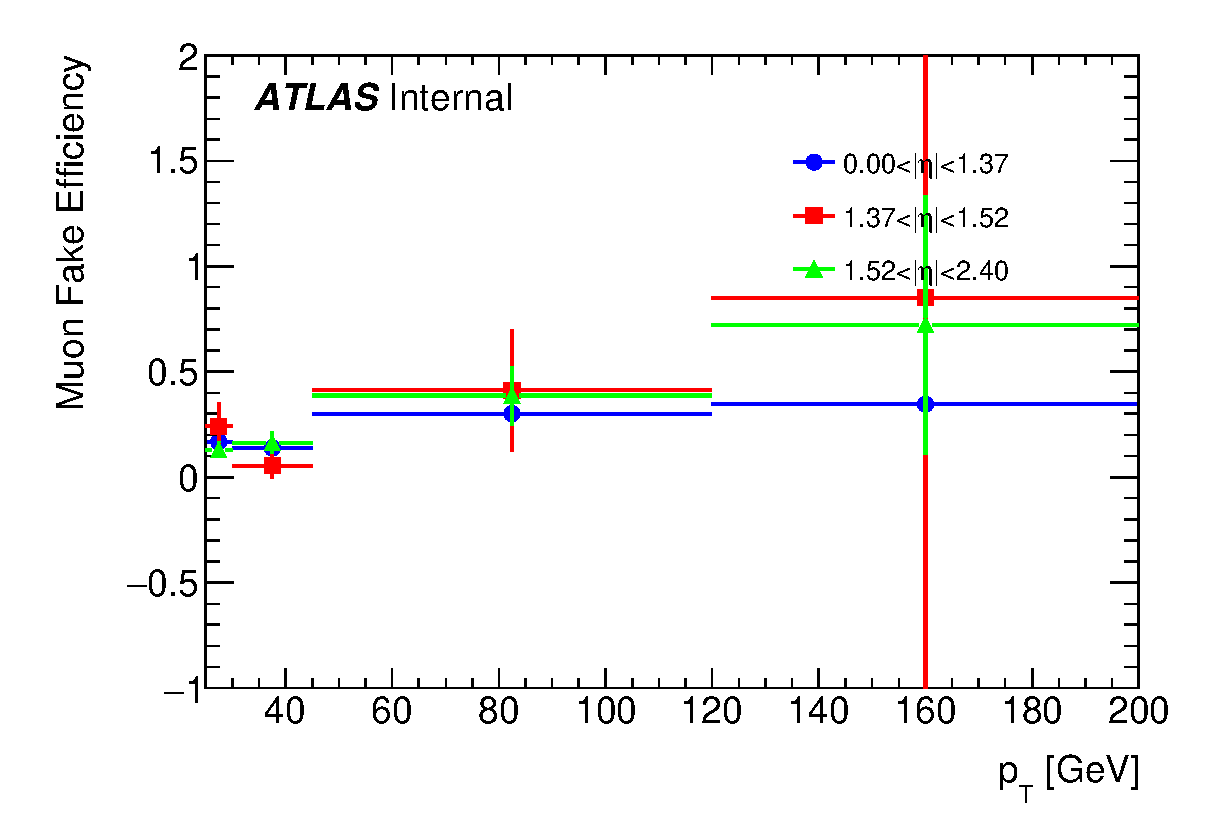
\includegraphics[width=0.49\linewidth]{data/plot/getFakeEffs/Mu_hEff.eps}
\caption{The fake efficiencies for electrons (left) and muons (right). Only statistical uncertainties are considered.}
\label{fig:result_fake_eff}
\end{figure}

\subsection{Validation for the fake lepton background}
In order to validate the fake lepton background, we compare data with all background predictions including the fake lepton background in validation regions.
The validation region is expected to have small contribution from signal.
It is defined as follows on top of the selections in section \ref{event_cleaning}.
\begin{itemize}
\item The two leptons are signal leptons.
\item The two leptons are same-sign.
\item b-jets veto: $n_{\text{b-jets}} = 0$, to suppress top background.
\item At least one signal jet: $n_{\text{jets}} \geq 1$
\item Z veto: $|m_{ll} - m_Z| > 10$ GeV, to suppress Z+jets background.
\item $E_{T}^{\text{miss}} > 30$ GeV
\item $m_{\text{eff}} > 200$ GeV
\end{itemize}

To ensure that the contribution from signal is small, the fractions of the signal contribution are checked in figure \ref{fig:signal_contribution_fakes}, and they are below 7\%.
In addition, in order to make sure that there is a substantial contribution from fake lepton background, the background compositions are checked in table \ref{tab:VRfakes_compos}.
The validation region is split into 3 channels: electron-electron, muon-muon and electron-muon channel.
Their fake contributions are 65\%,  24\% and 48\% respectively.

The backgrounds and the data are compared in several variable distributions in the 3 channels, shown in figures \ref{fig:VRSS_fake_ee}, \ref{fig:VRSS_fake_mumu} and \ref{fig:VRSS_fake_emu} respectively.
There are good agreements between the backgrounds and the data within the uncertainties.

\begin{figure}[htbp]
\begin{center}
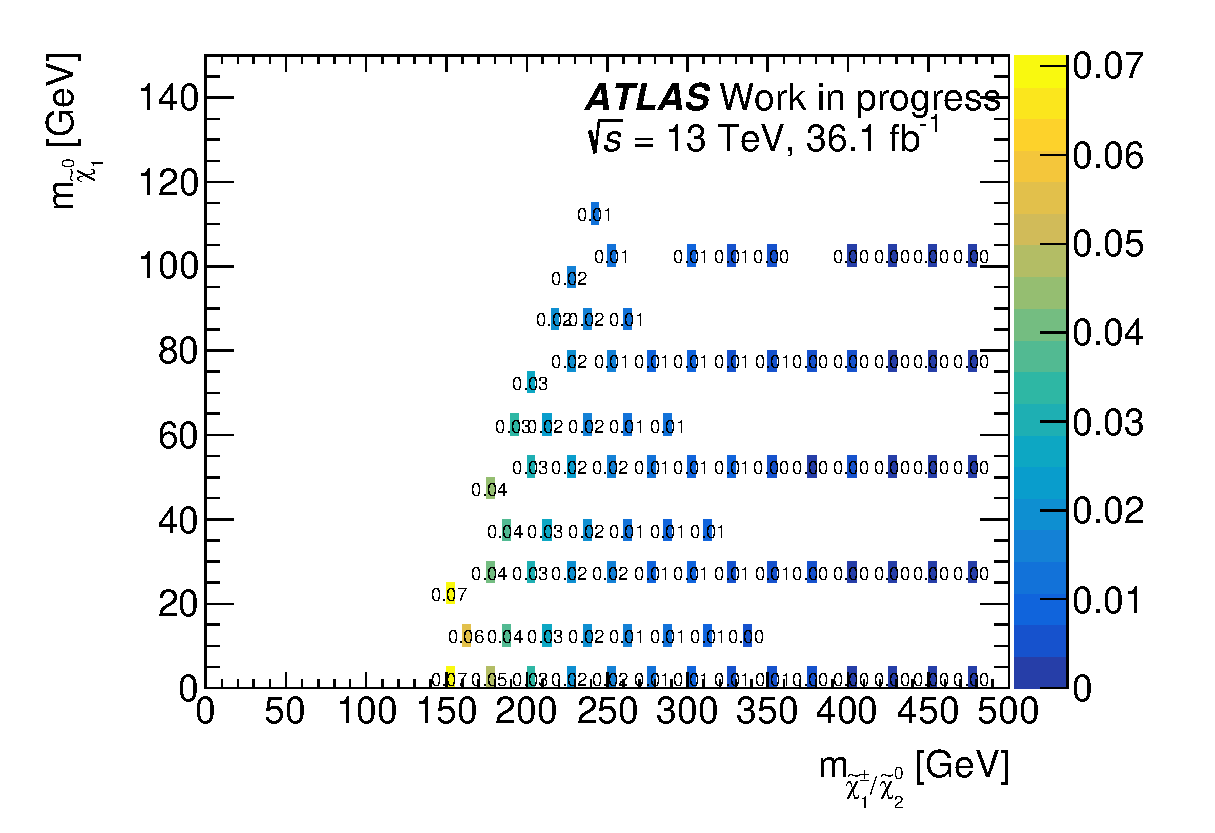
\includegraphics[width=\textwidth]{data/plot/Fake_VR/signal_contamination}
\caption{Signal contributions in the validation region are shown for different mass points.}
\label{fig:signal_contribution_fakes}
\end{center}
\end{figure}

\begin{table}[htbp]
\begin{center}
\begin{tabular}{|c|c|c|c|}
\hline
\hline
& ee channel & $\mu\mu$ channel & e$\mu$ channel\\
\hline
\hline
Fakes       & 65.1\% (860.7) & 23.6\% (96.2)  & 47.8\% (614.7) \\
Charge Flip & 12.7\% (168.0) &  0.0\% (0.0)   &  2.6\% (34.0)  \\
WZ          & 15.2\% (201.1) & 51.2\% (209.2) & 35.0\% (450.7) \\
ZZ          &  0.6\% (8.4)   &  2.3\% (9.5)   &  1.6\% (20.4)  \\
WW          &  3.4\% (45.2)  & 13.1\% (53.7)  &  7.6\% (98.3)  \\
Rare        &  2.3\% (30.8)  &  7.5\% (30.5)  &  3.9\% (50.0)  \\
ttV         &  0.6\% (8.3)   &  2.3\% (9.4)   &  1.4\% (18.1)  \\
\hline
Total BG    & 1322           & 408.4          & 1286 \\
\hline
Data        & 1201           & 454            & 1410 \\
\hline
\end{tabular}
\caption{The background compositions in the validation region. The numbers in brackets are the event yields.}
\label{tab:VRfakes_compos}
\end{center}
\end{table}

\begin{figure}[htbp]
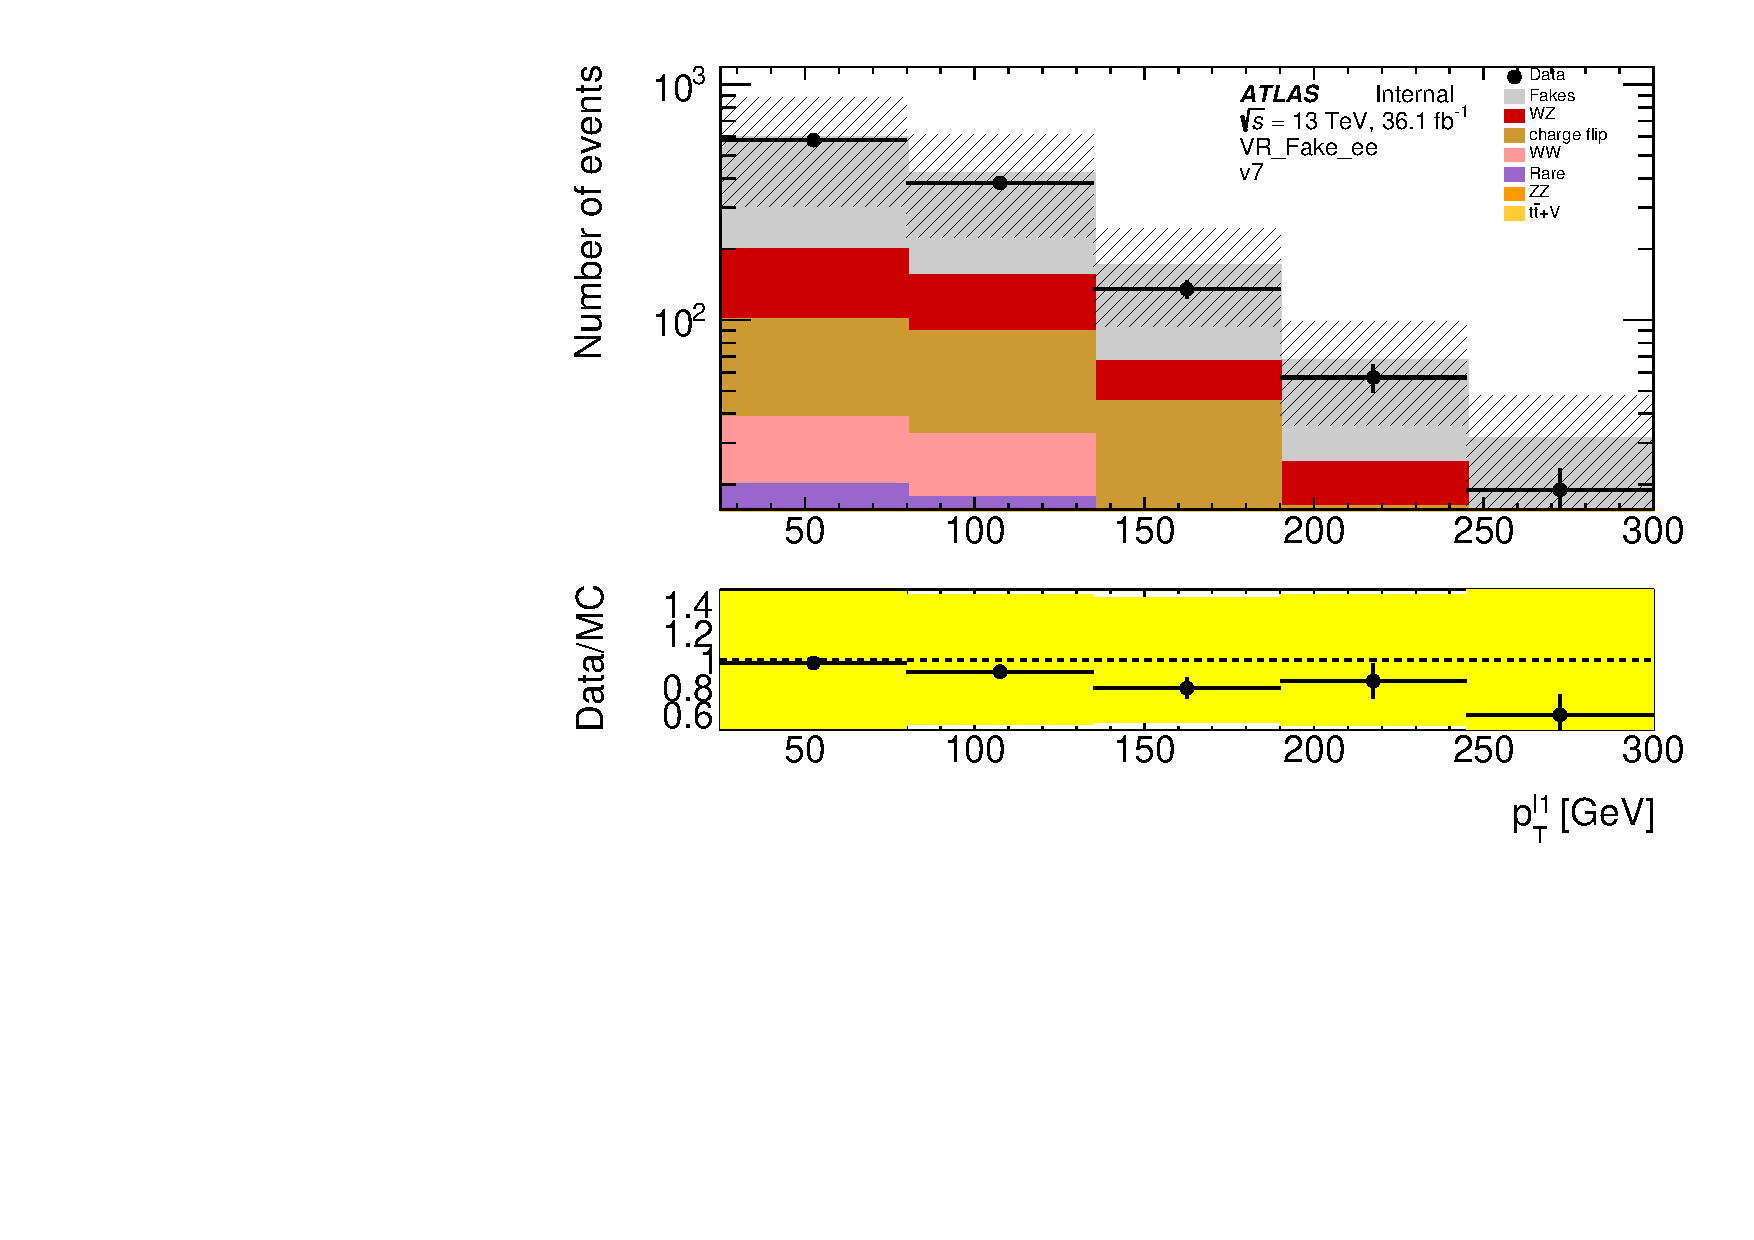
\includegraphics[width=0.49\textwidth]{data/plot/Fake_VR/pt1_VR_Fake_ee}
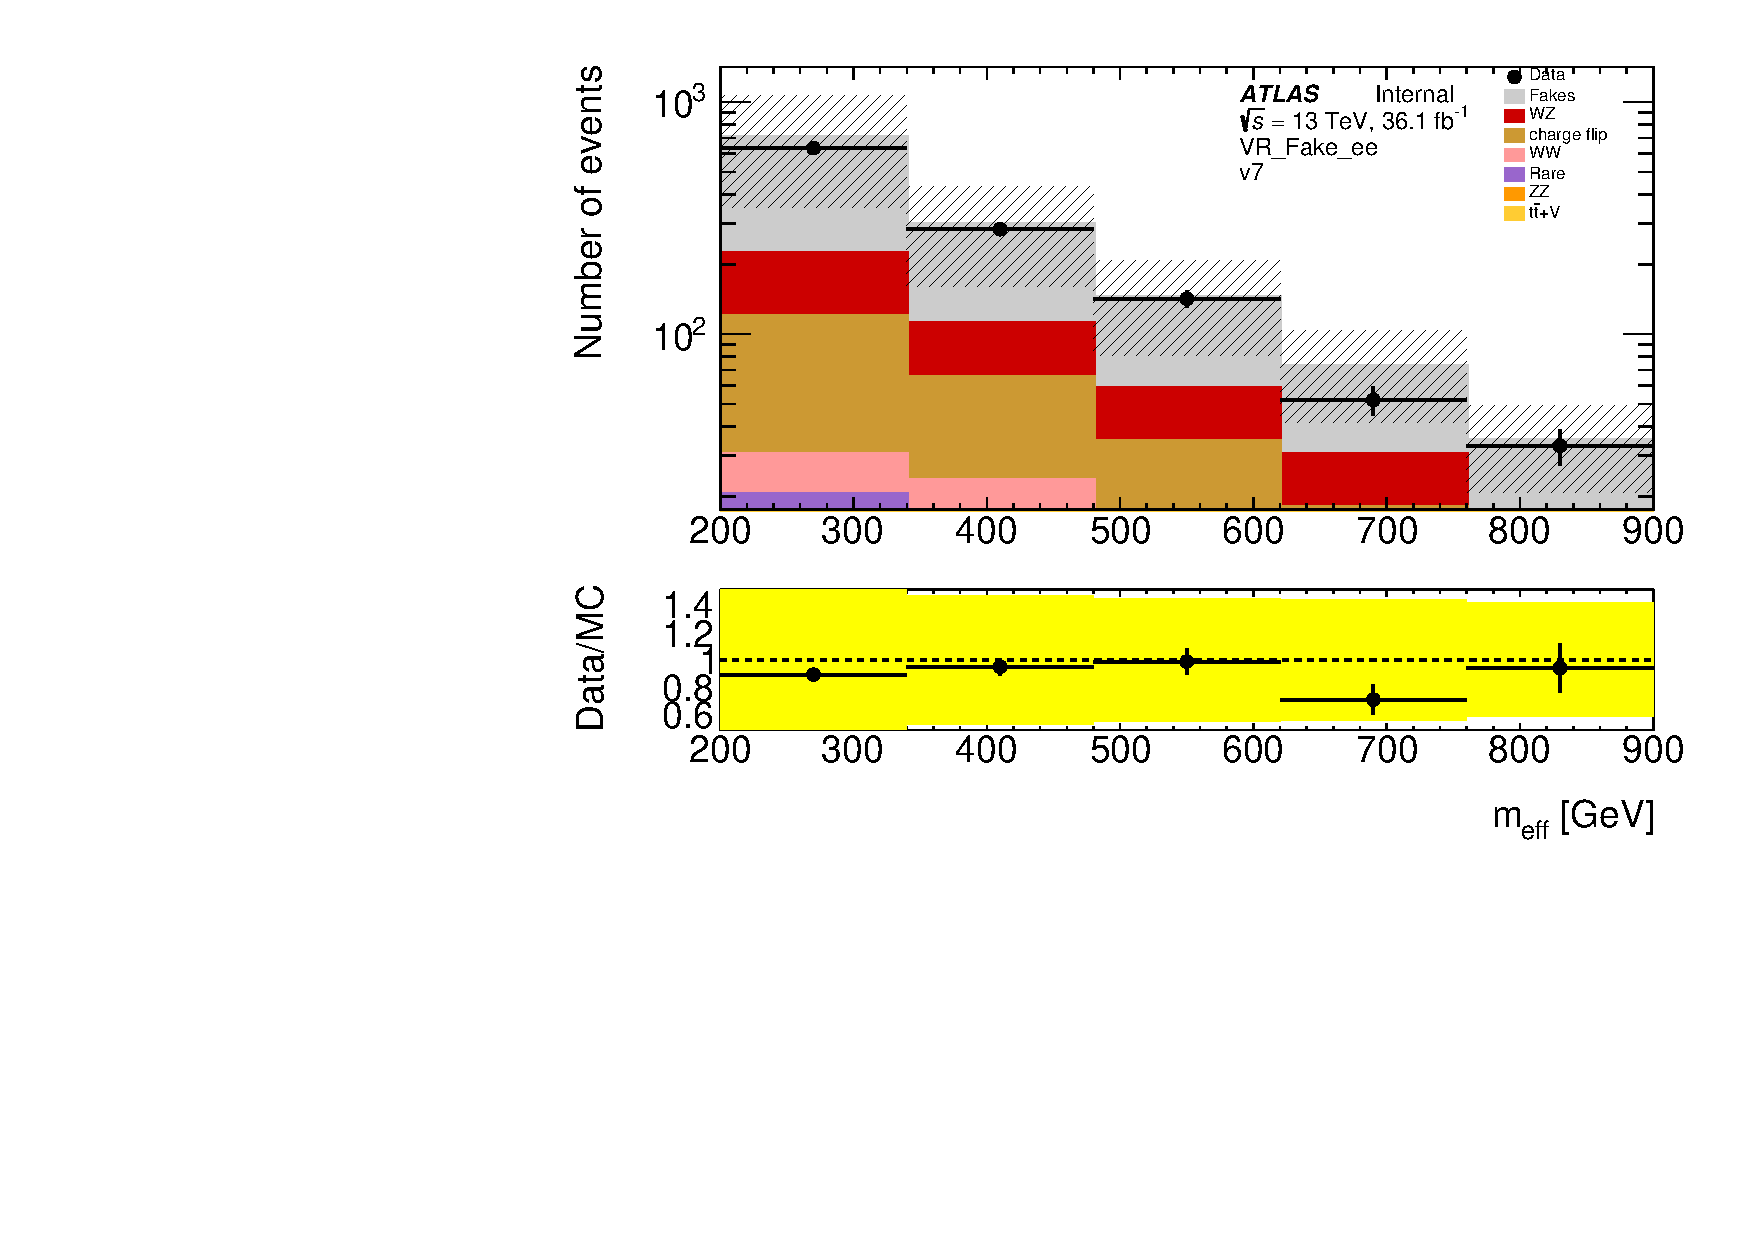
\includegraphics[width=0.49\textwidth]{data/plot/Fake_VR/meff_VR_Fake_ee}\\
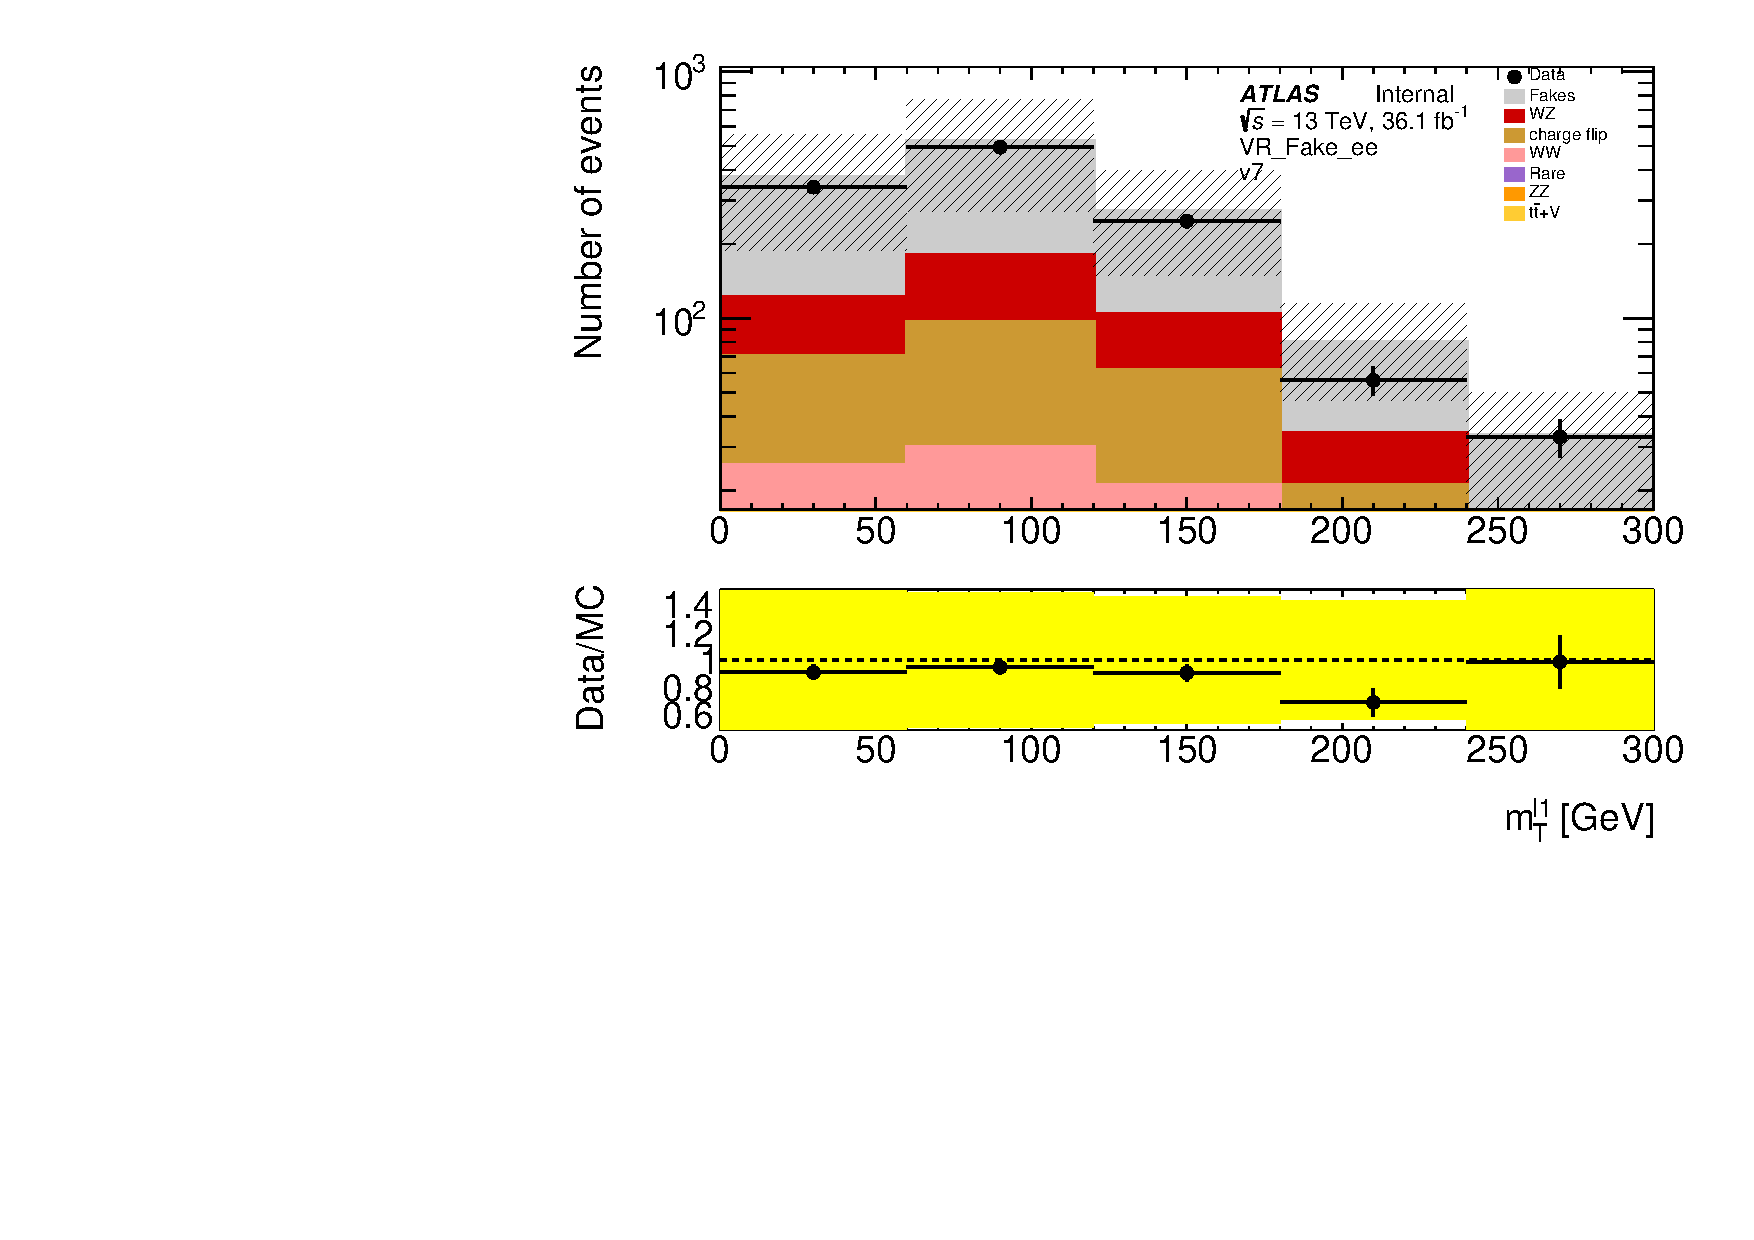
\includegraphics[width=0.49\textwidth]{data/plot/Fake_VR/mt1_VR_Fake_ee}
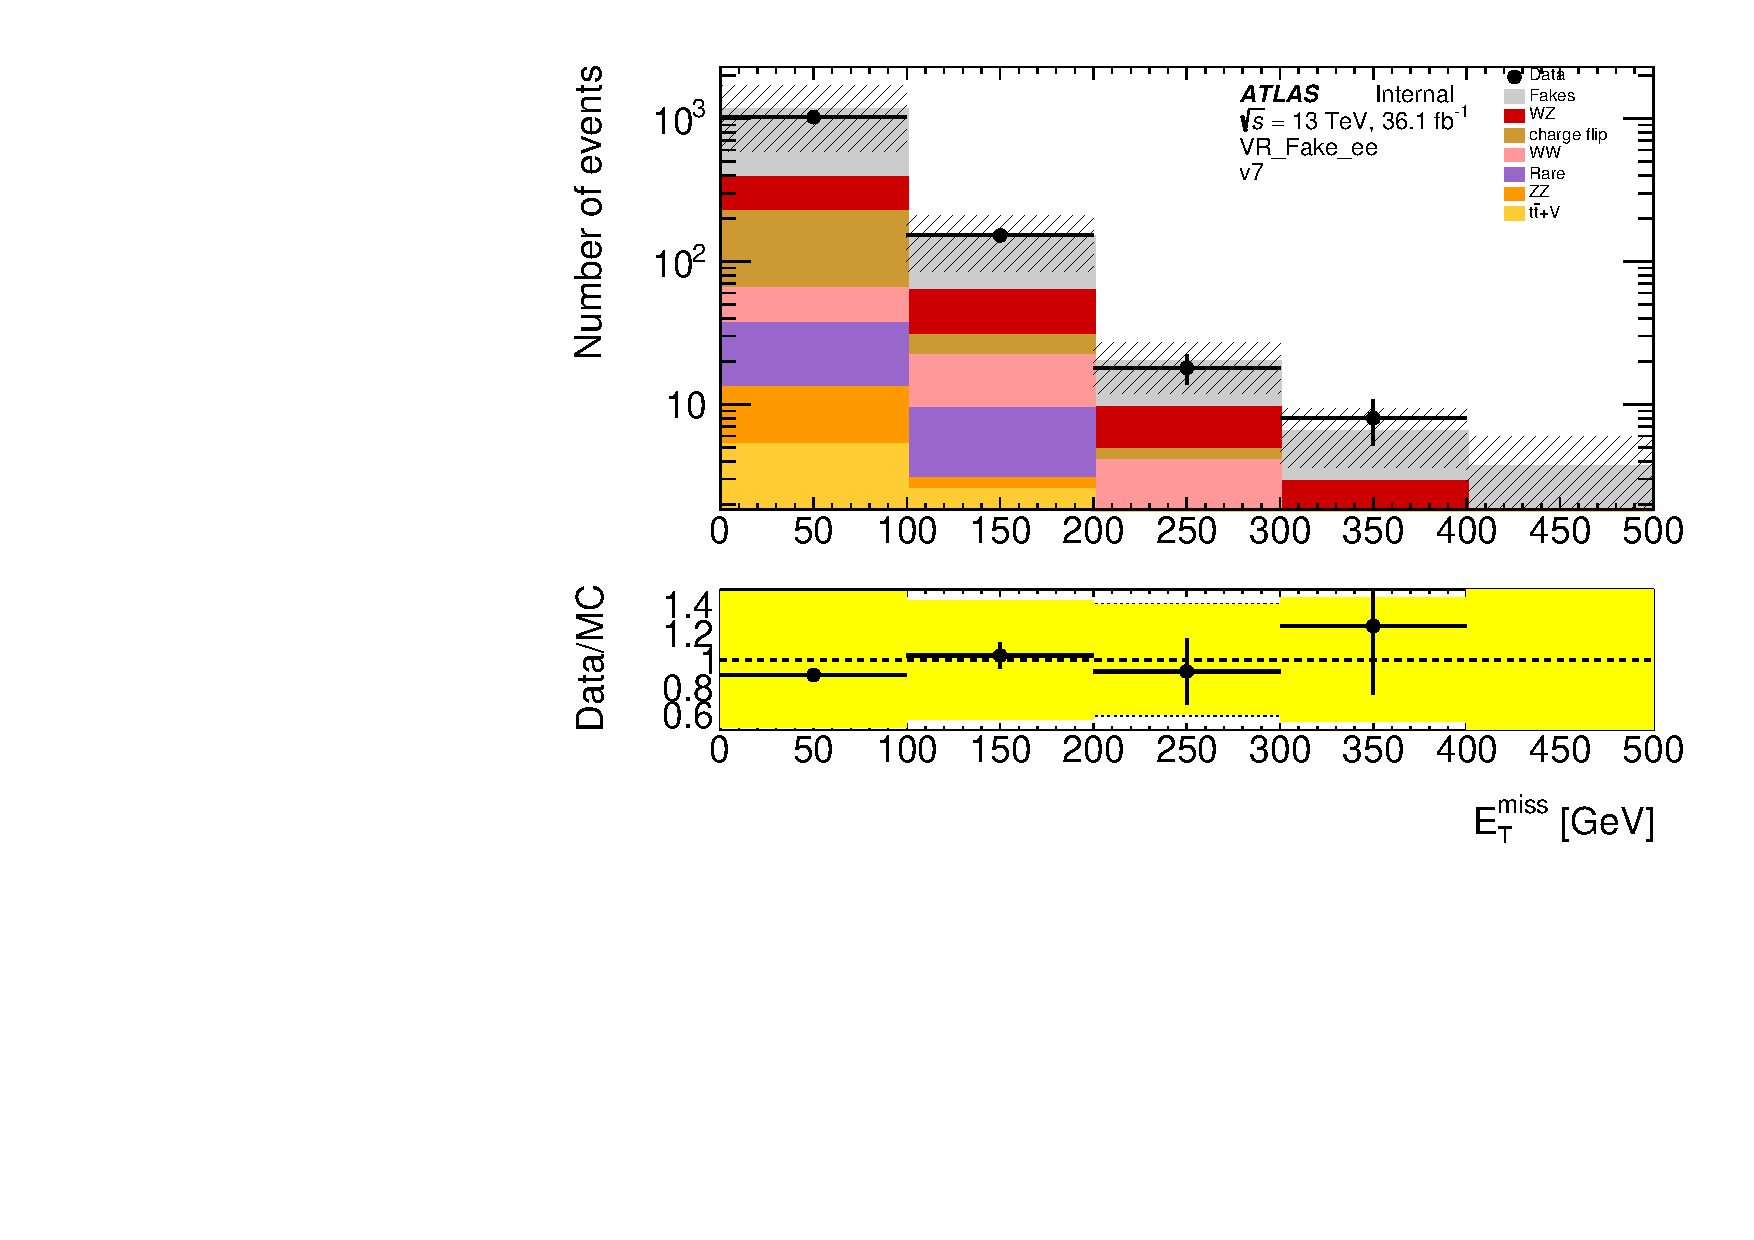
\includegraphics[width=0.49\textwidth]{data/plot/Fake_VR/MET_VR_Fake_ee}\\
\begin{center}
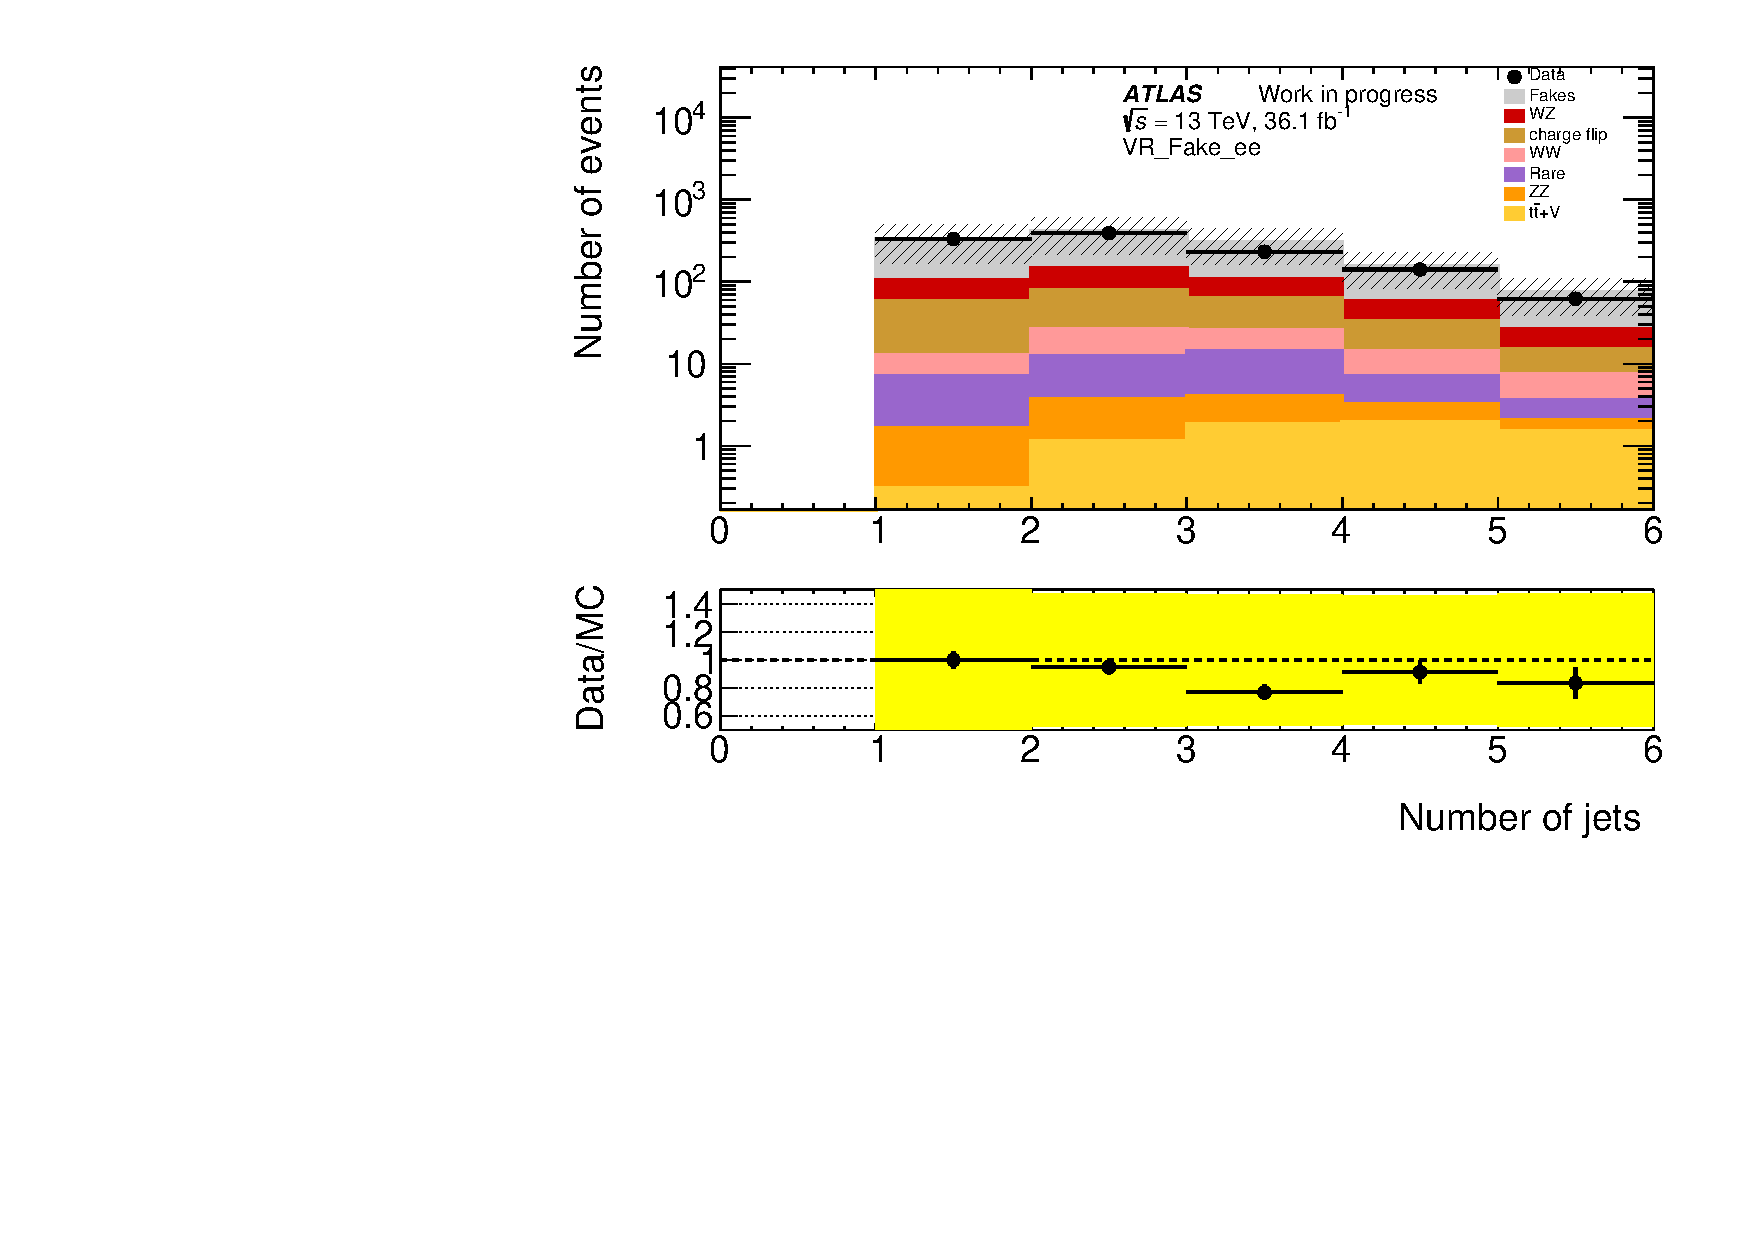
\includegraphics[width=0.49\textwidth]{data/plot/Fake_VR/nJet_VR_Fake_ee}
\end{center}
\caption{Distribution of the  leading lepton $p_T$, $m_{\text{eff}}$, $m_T$, $E_{T}^{\text{miss}}$ and $n_{\text{jets}}$ in the electron-electron channel. The ratio of data to background yields is shown in the lower plot. The error bar includes all the systematic uncertainties except for the theoretical uncertainties.}
\label{fig:VRSS_fake_ee}
\end{figure}

\begin{figure}[htbp]
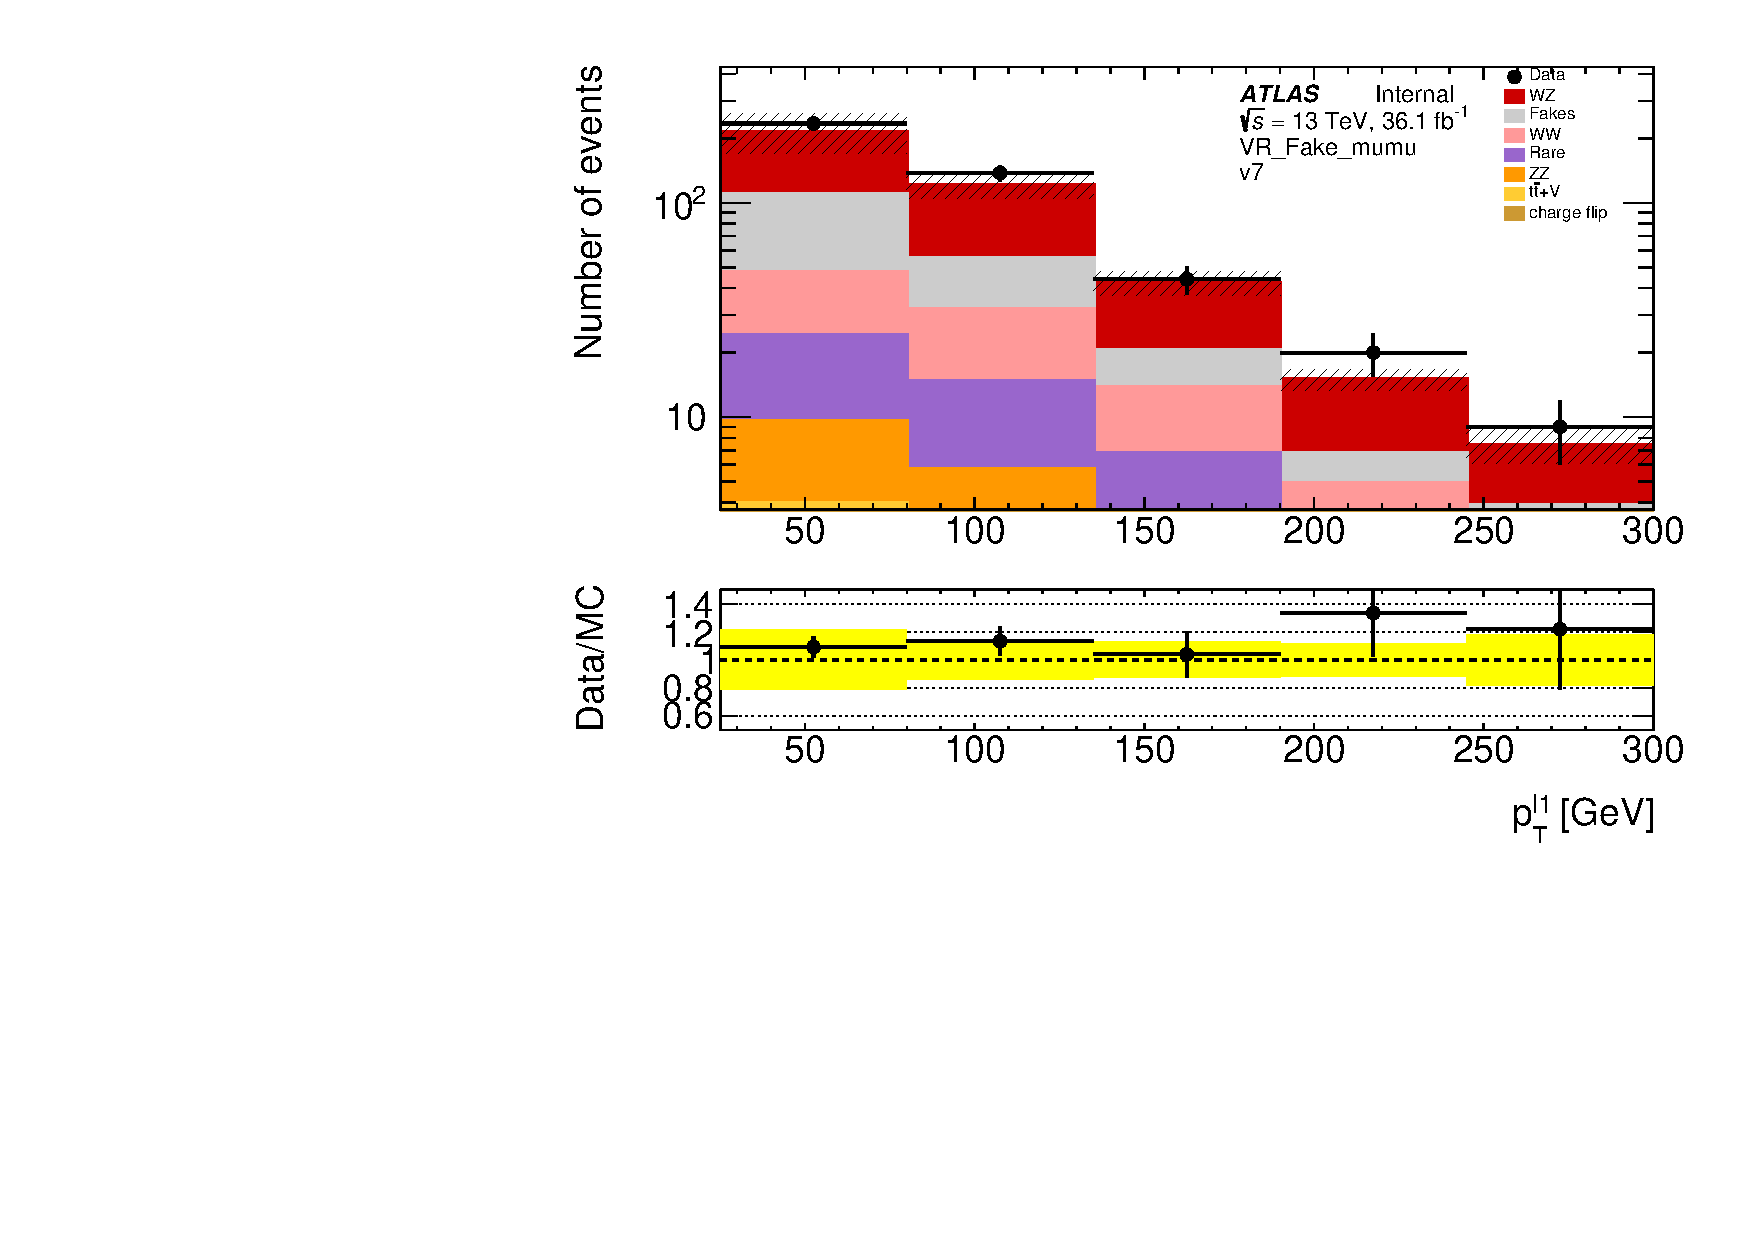
\includegraphics[width=0.49\textwidth]{data/plot/Fake_VR/pt1_VR_Fake_mumu}
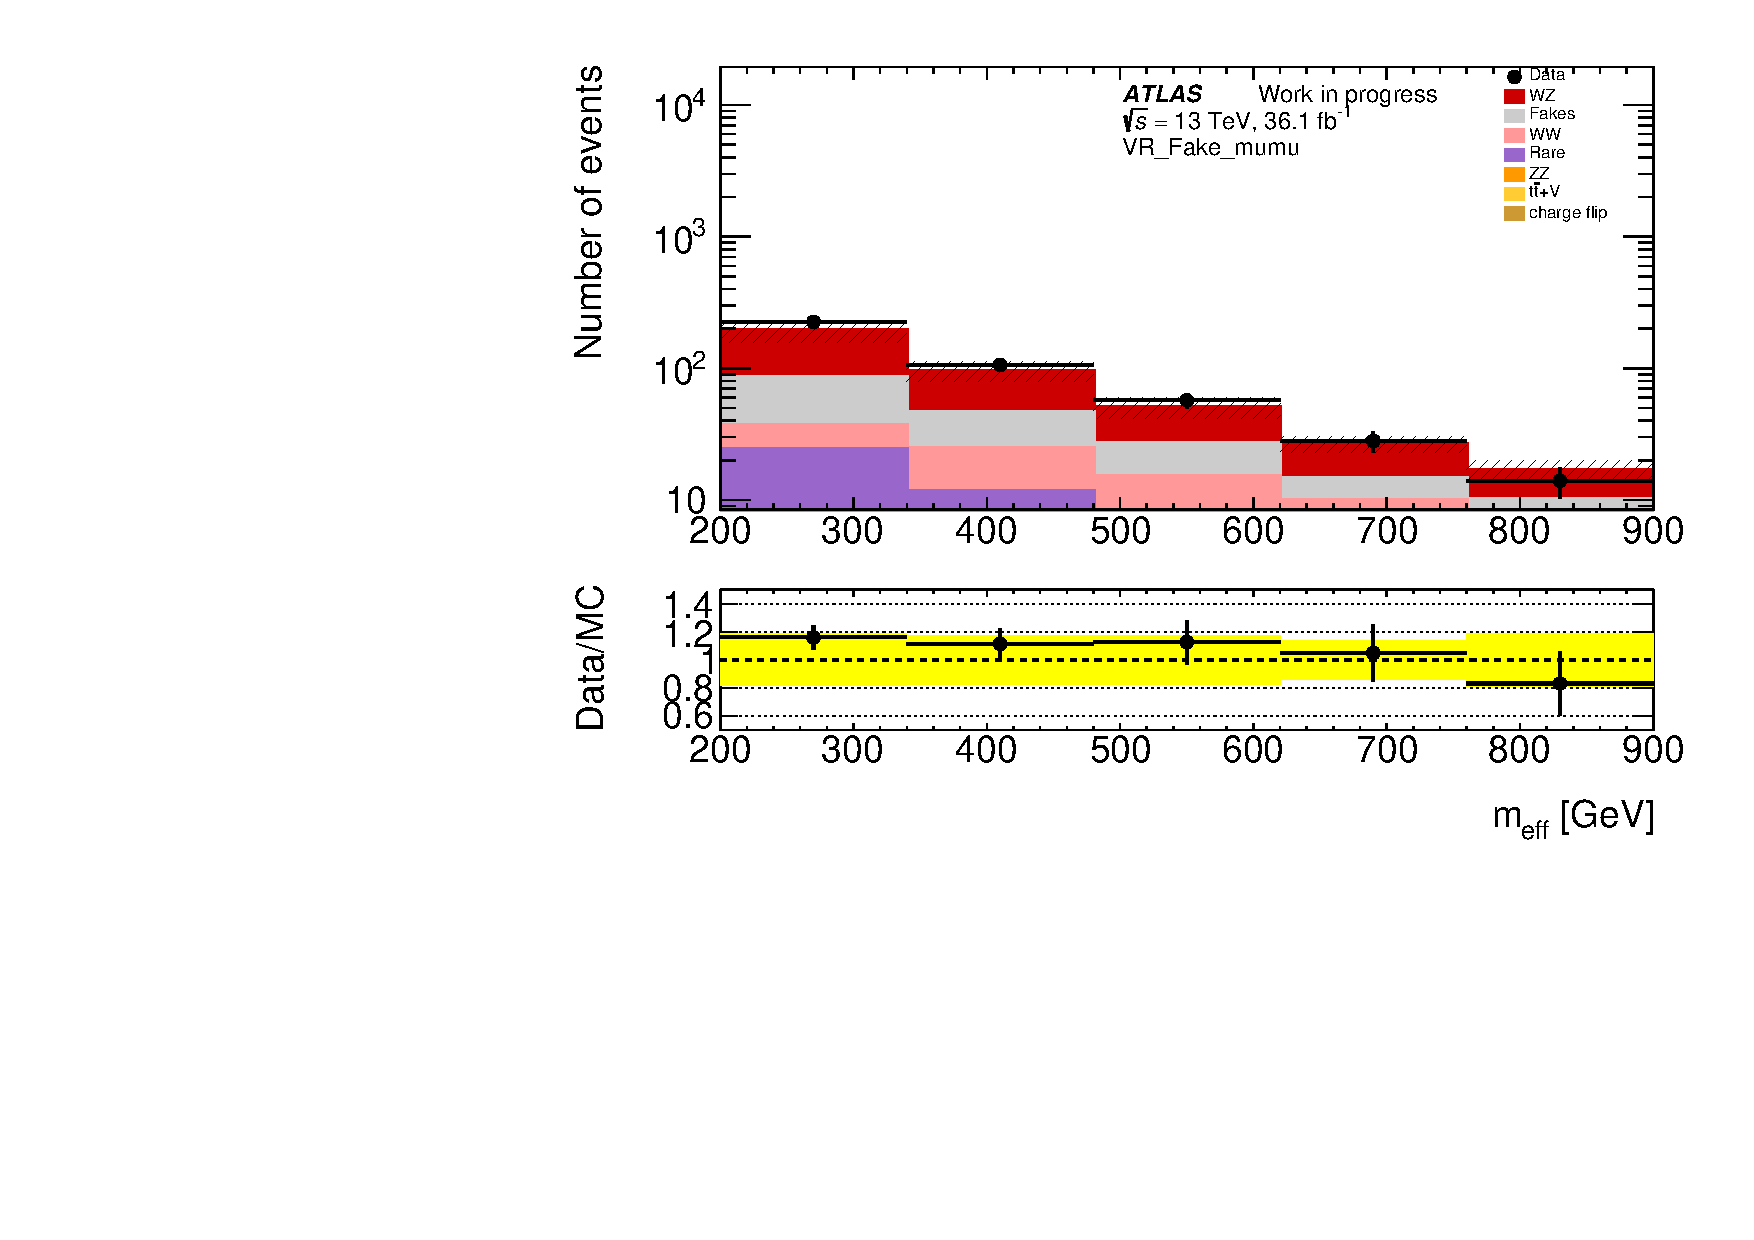
\includegraphics[width=0.49\textwidth]{data/plot/Fake_VR/meff_VR_Fake_mumu}\\
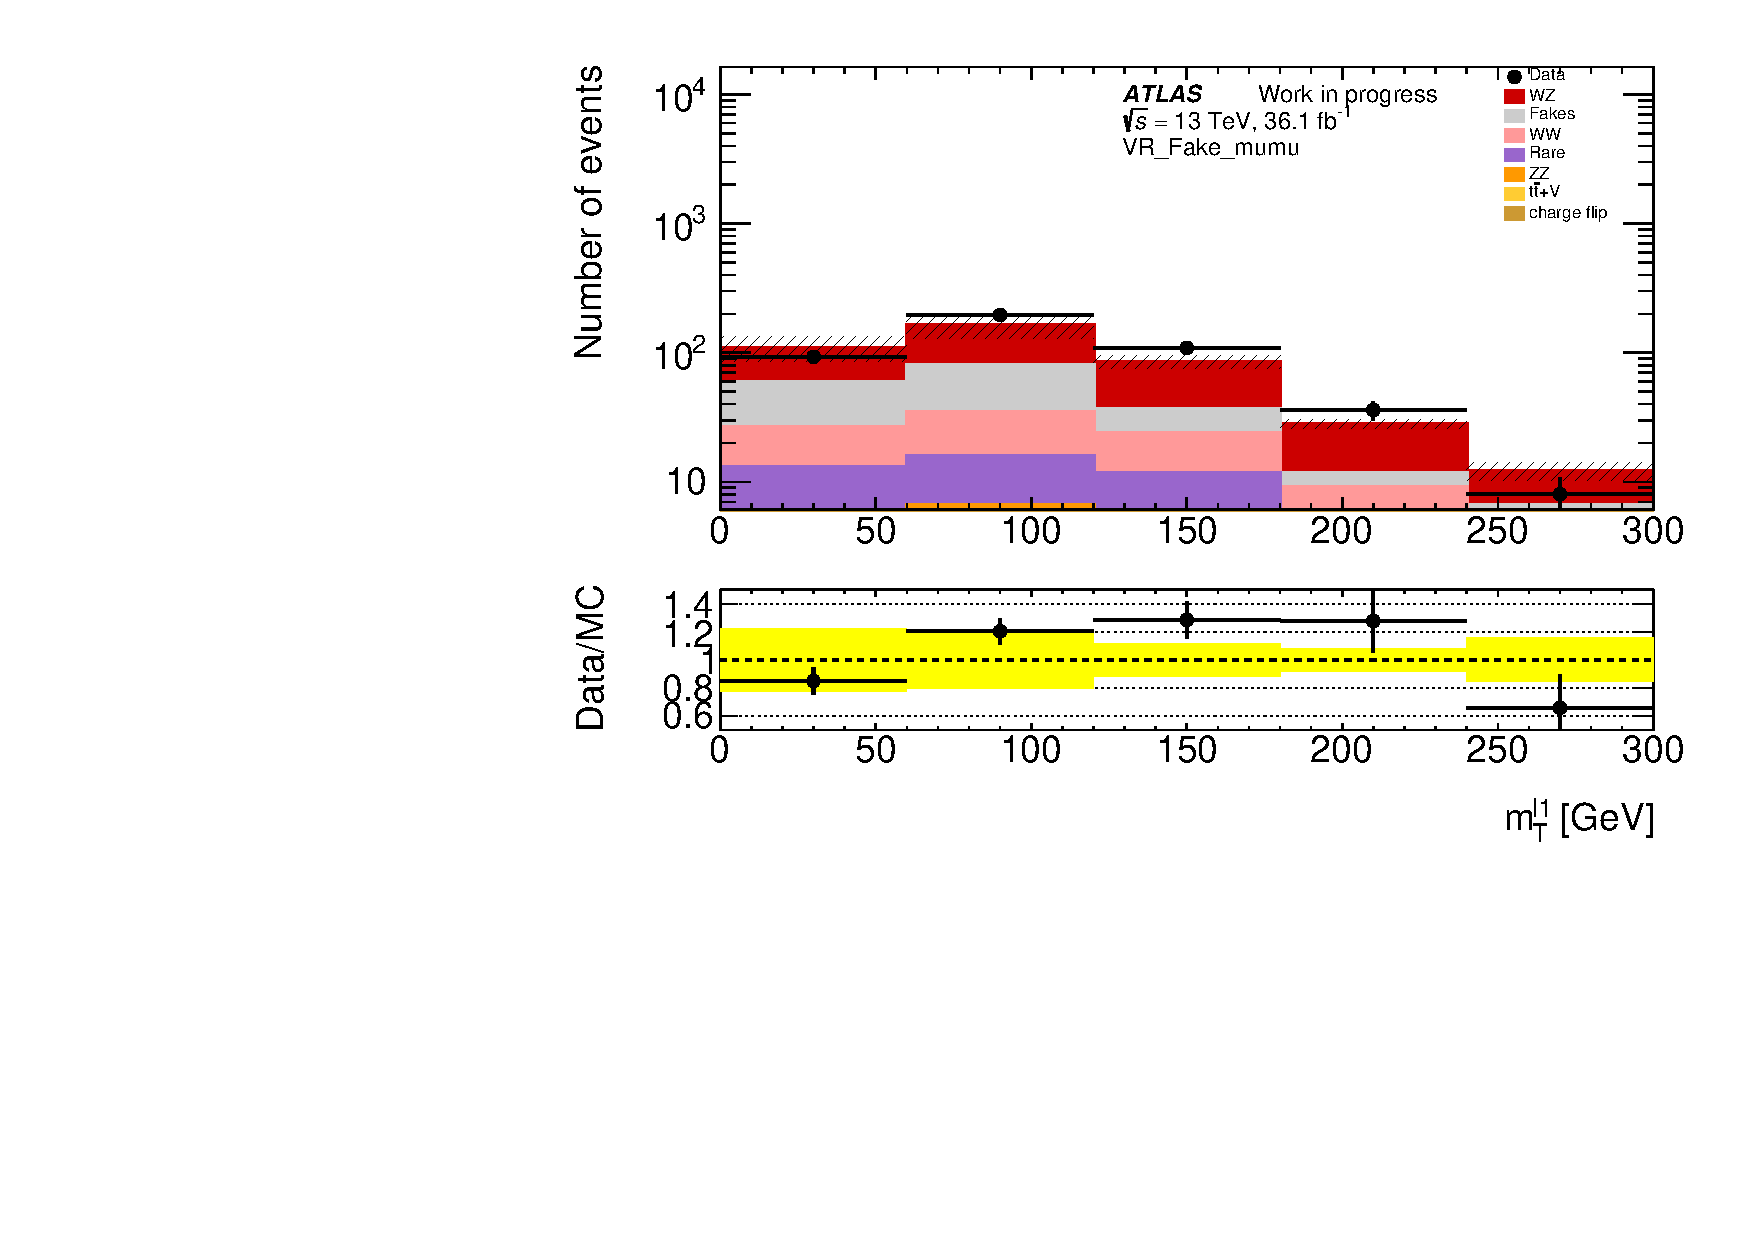
\includegraphics[width=0.49\textwidth]{data/plot/Fake_VR/mt1_VR_Fake_mumu}
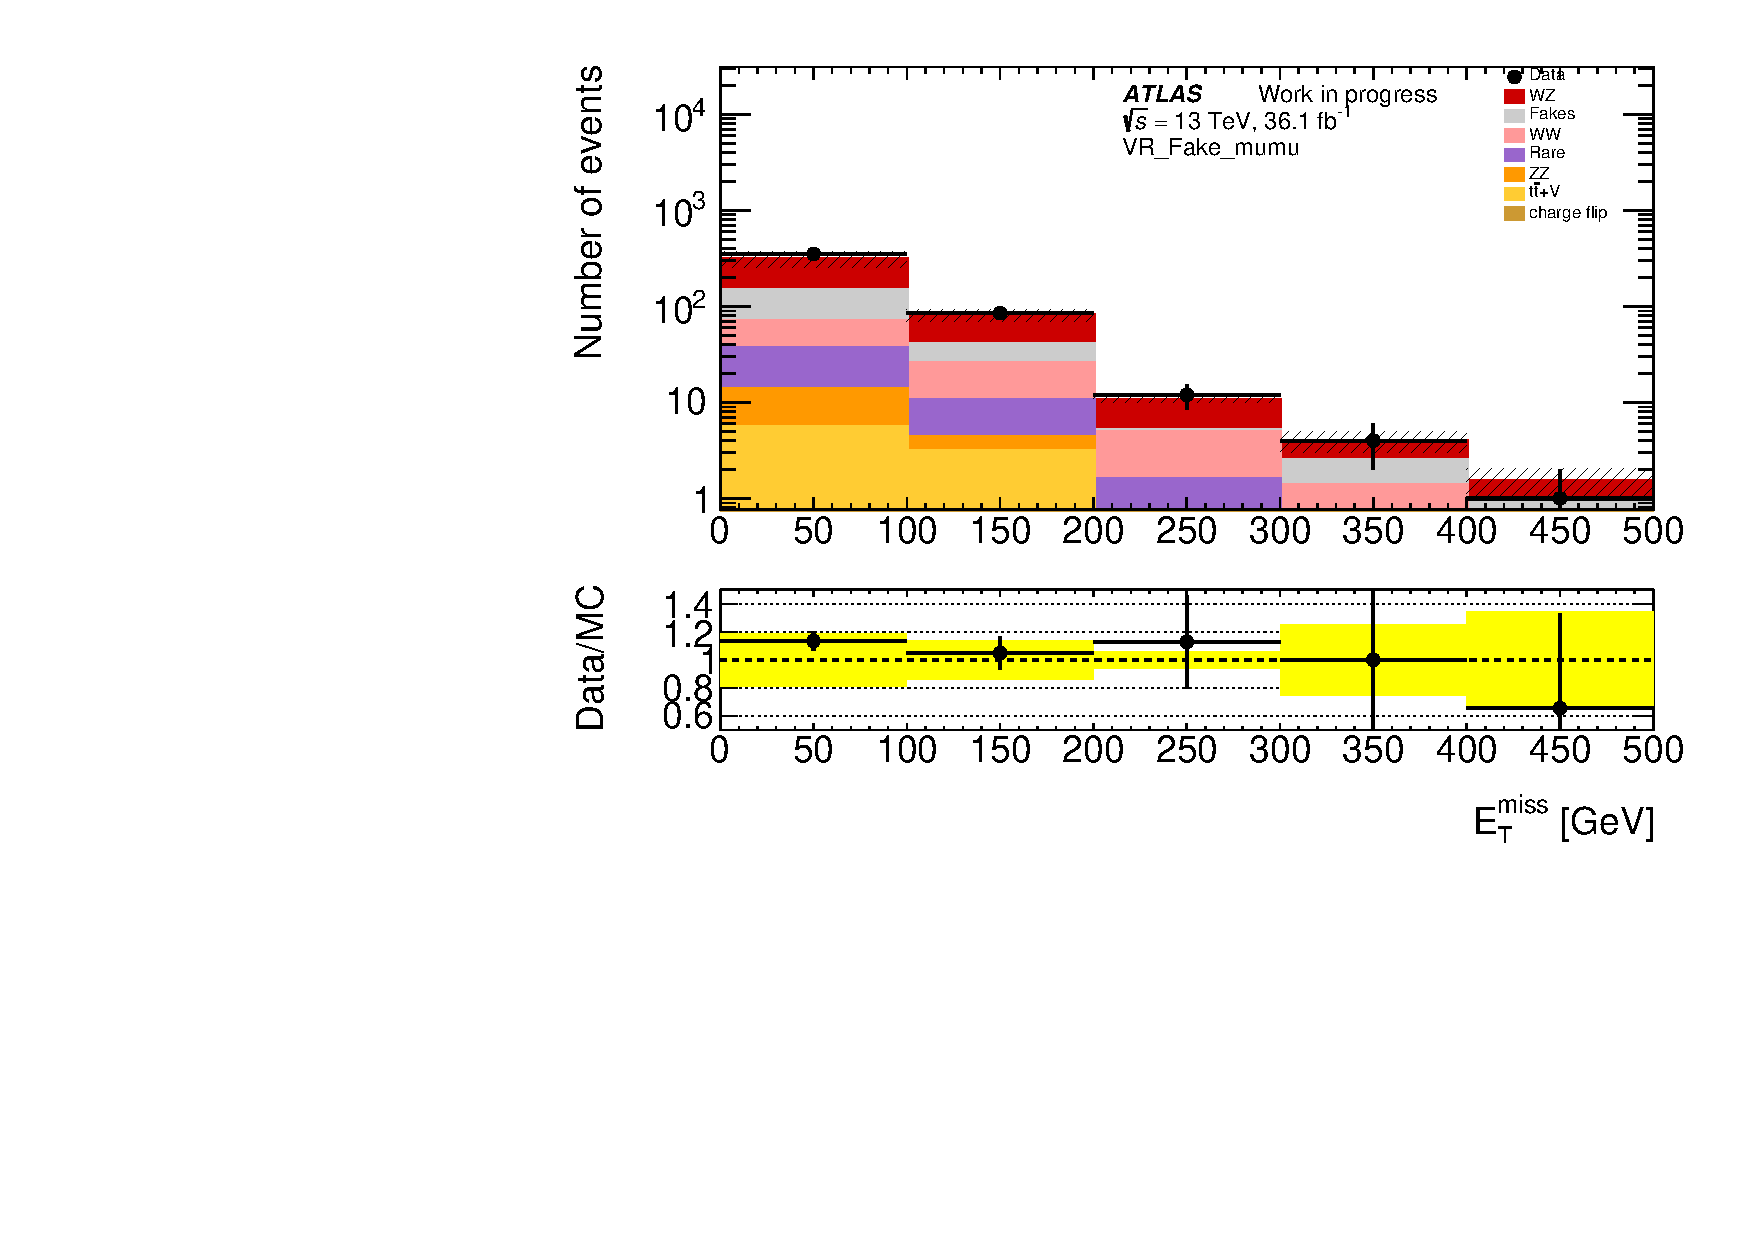
\includegraphics[width=0.49\textwidth]{data/plot/Fake_VR/MET_VR_Fake_mumu}\\
\begin{center}
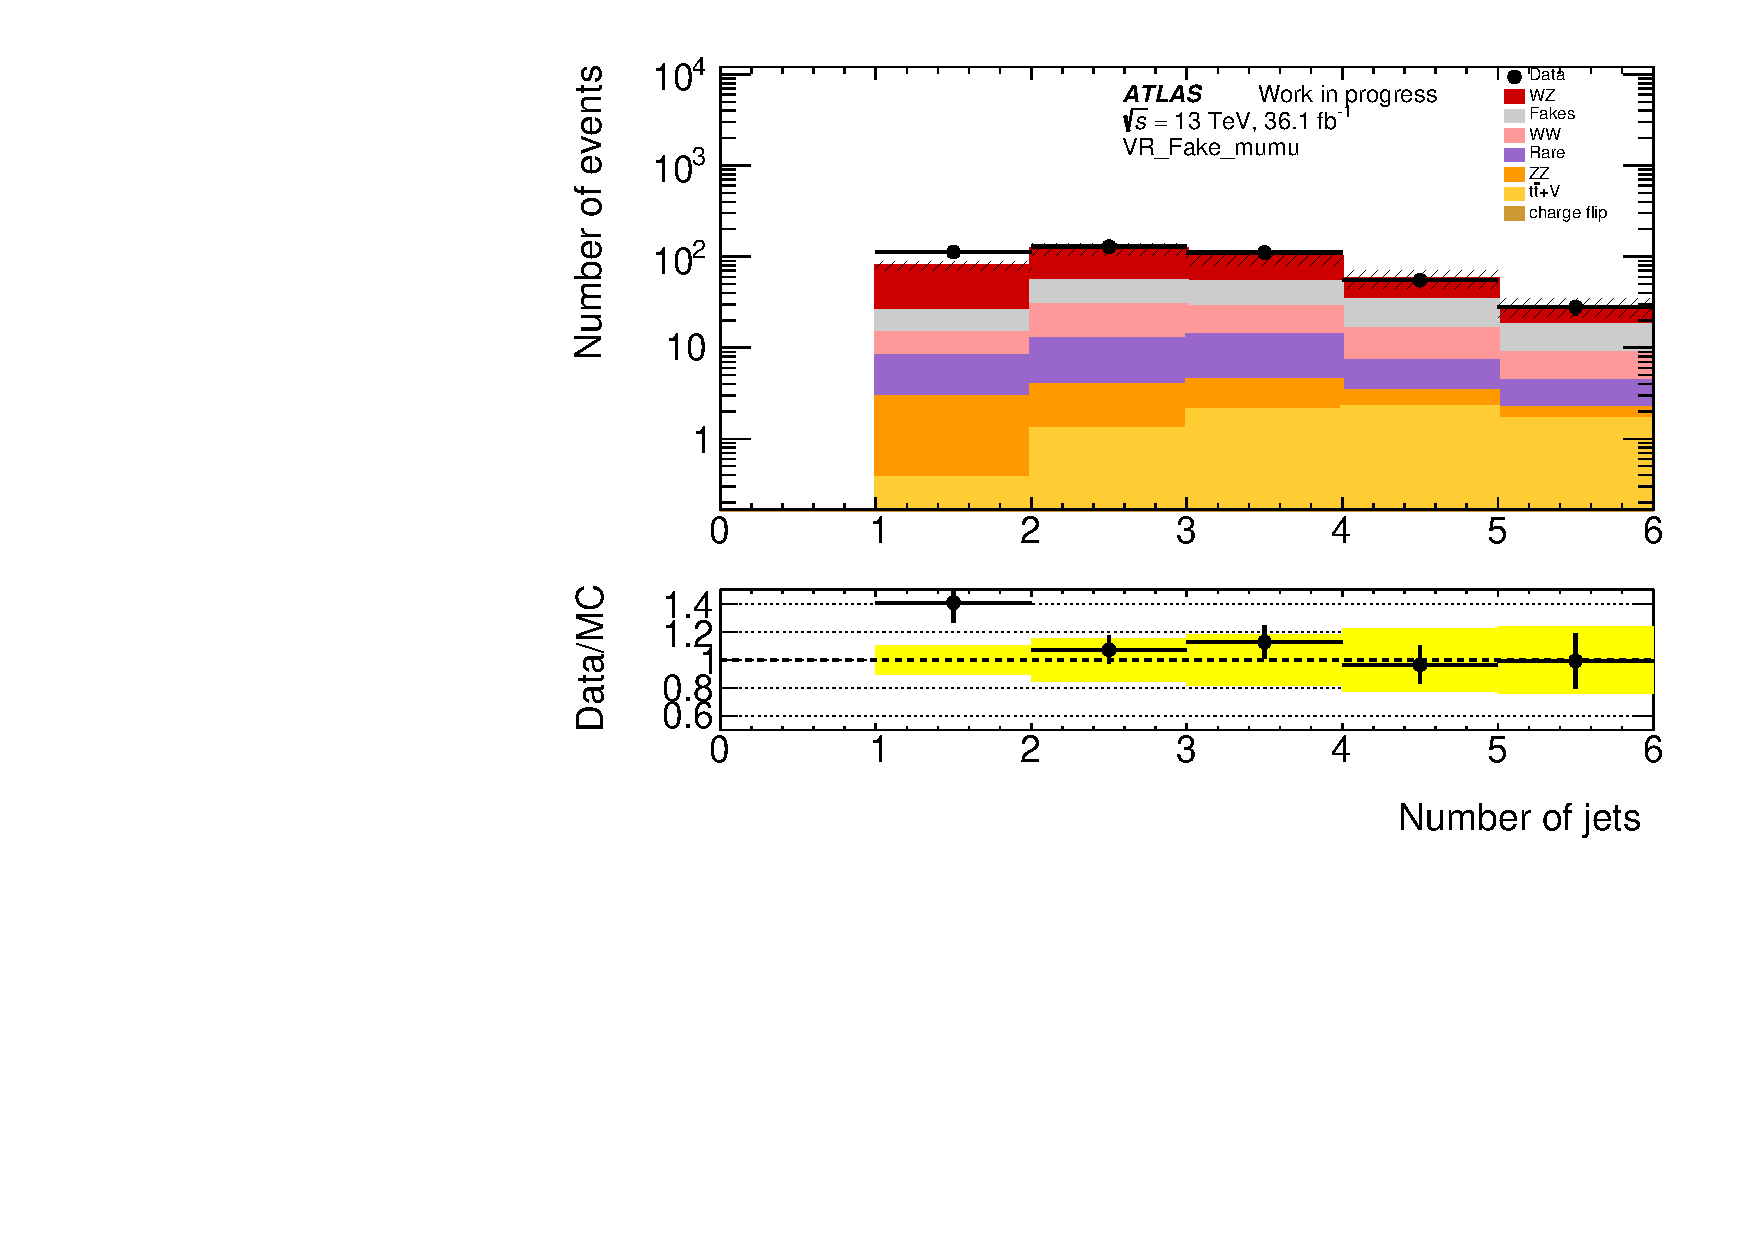
\includegraphics[width=0.49\textwidth]{data/plot/Fake_VR/nJet_VR_Fake_mumu}
\end{center}
\caption{Distribution of the  leading lepton $p_T$, $m_{\text{eff}}$, $m_T$, $E_{T}^{\text{miss}}$ and $n_{\text{jets}}$ in the muon-muon channel. The ratio of data to background yields is shown in the lower plot. The error bar includes all the systematic uncertainties except for the theoretical uncertainties.}
\label{fig:VRSS_fake_mumu}
\end{figure}

\begin{figure}[htbp]
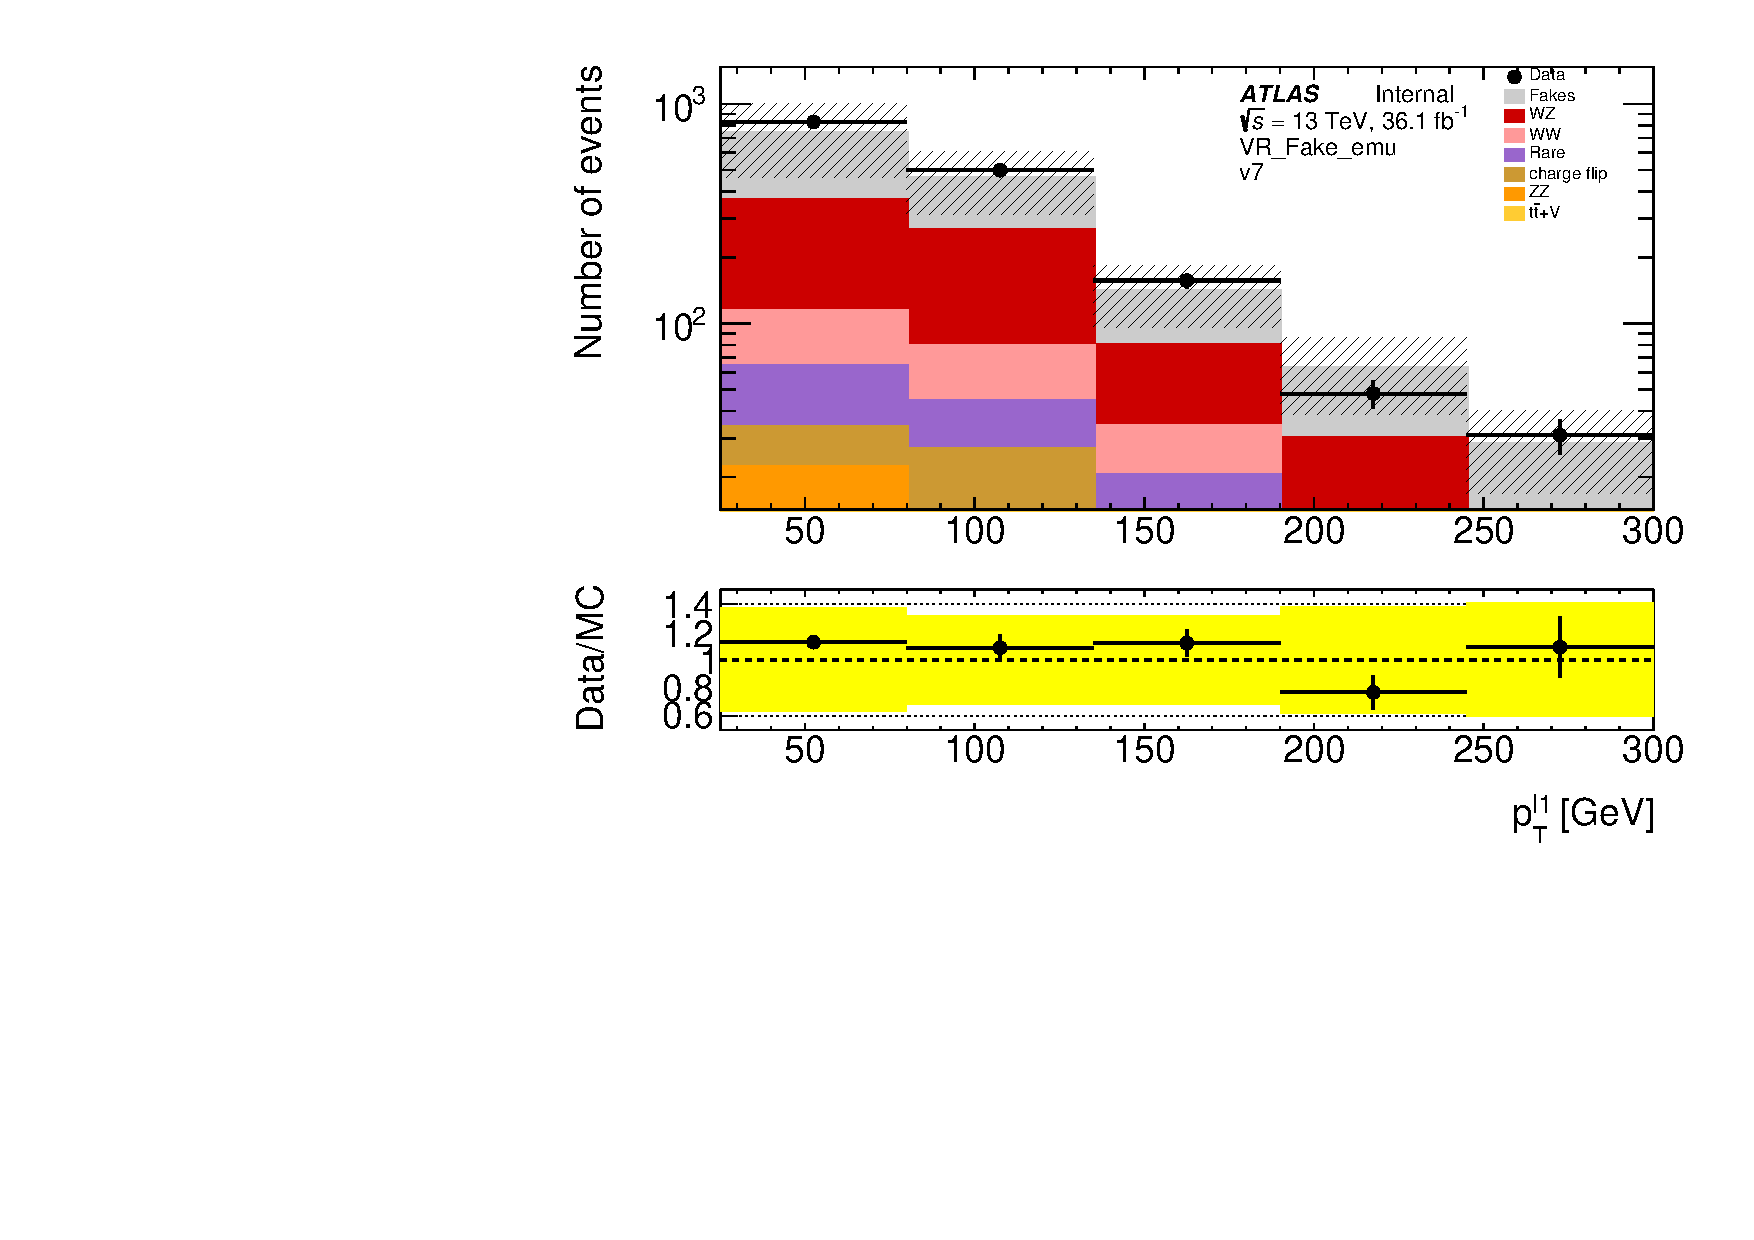
\includegraphics[width=0.49\textwidth]{data/plot/Fake_VR/pt1_VR_Fake_emu}
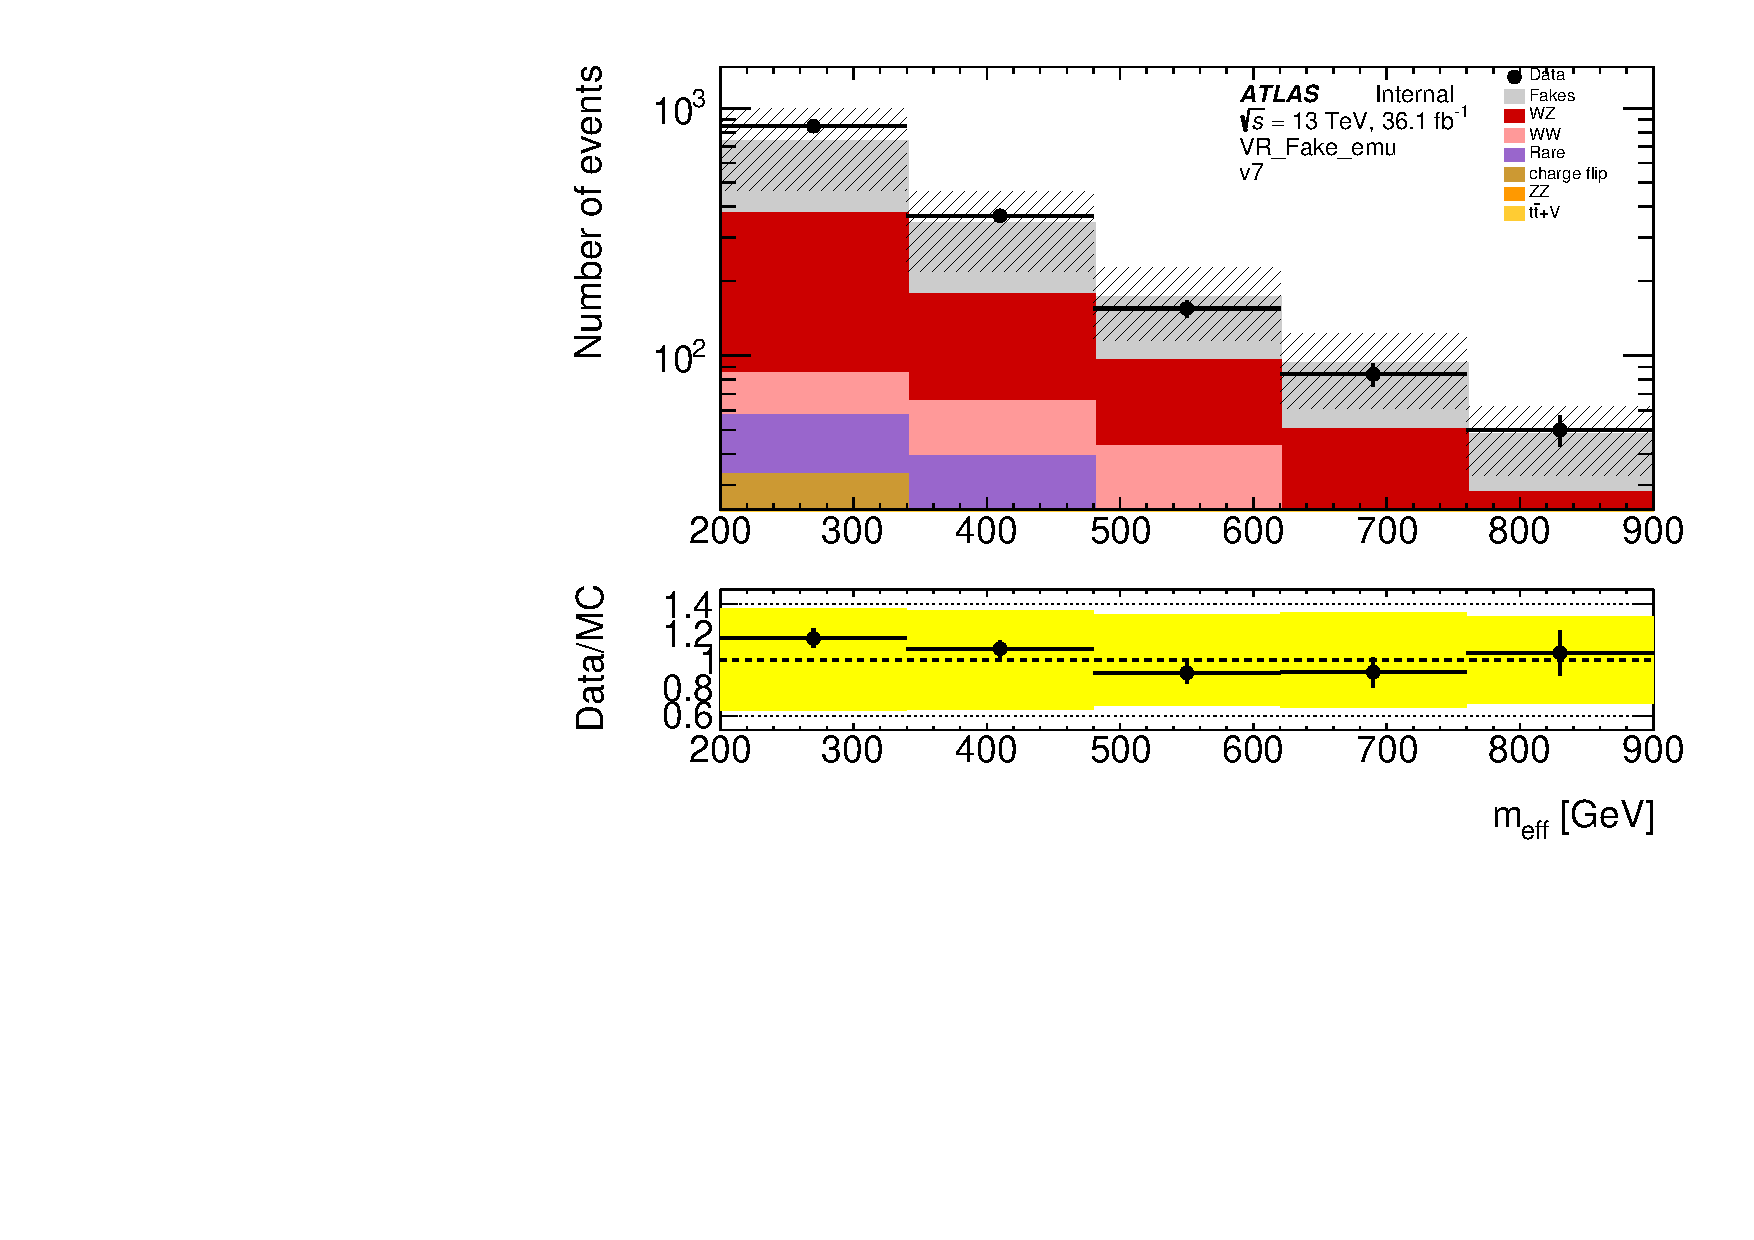
\includegraphics[width=0.49\textwidth]{data/plot/Fake_VR/meff_VR_Fake_emu}\\
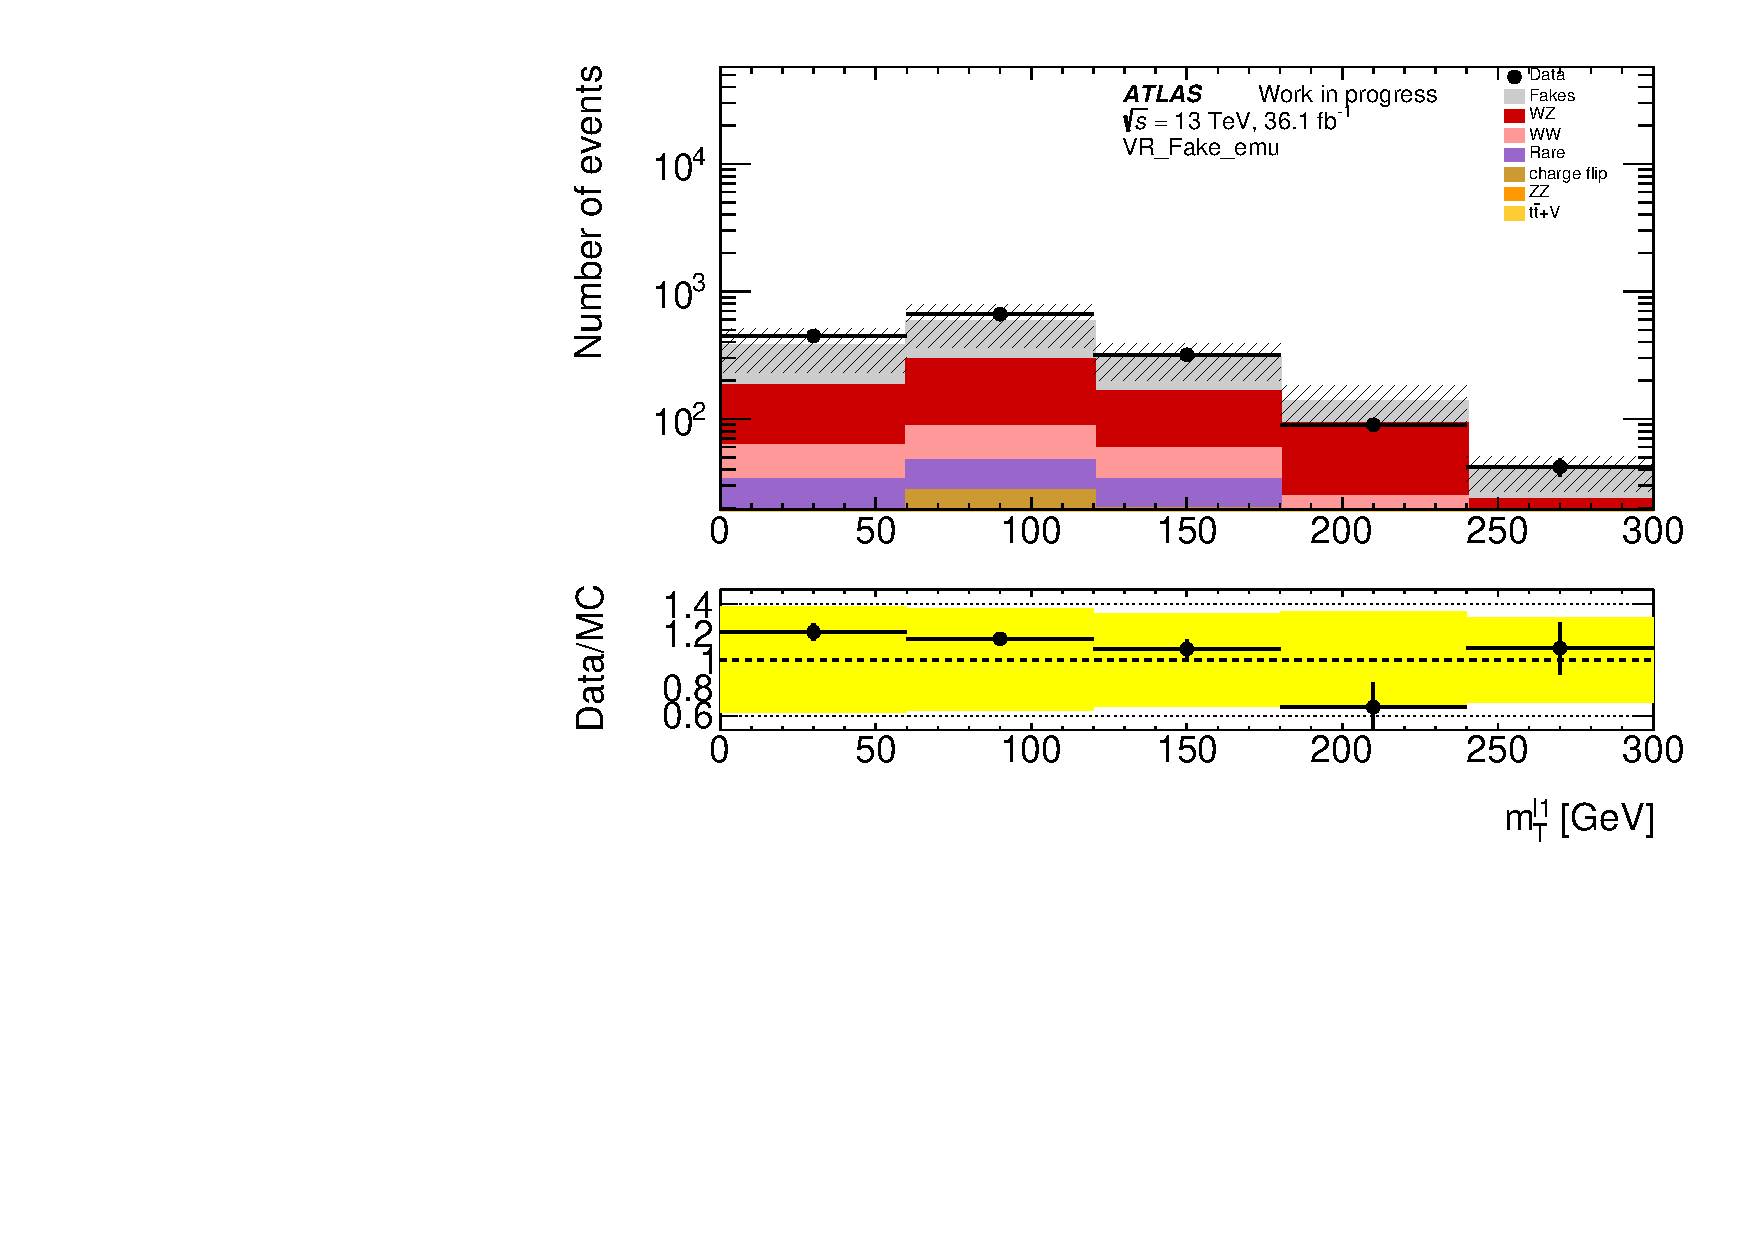
\includegraphics[width=0.49\textwidth]{data/plot/Fake_VR/mt1_VR_Fake_emu}
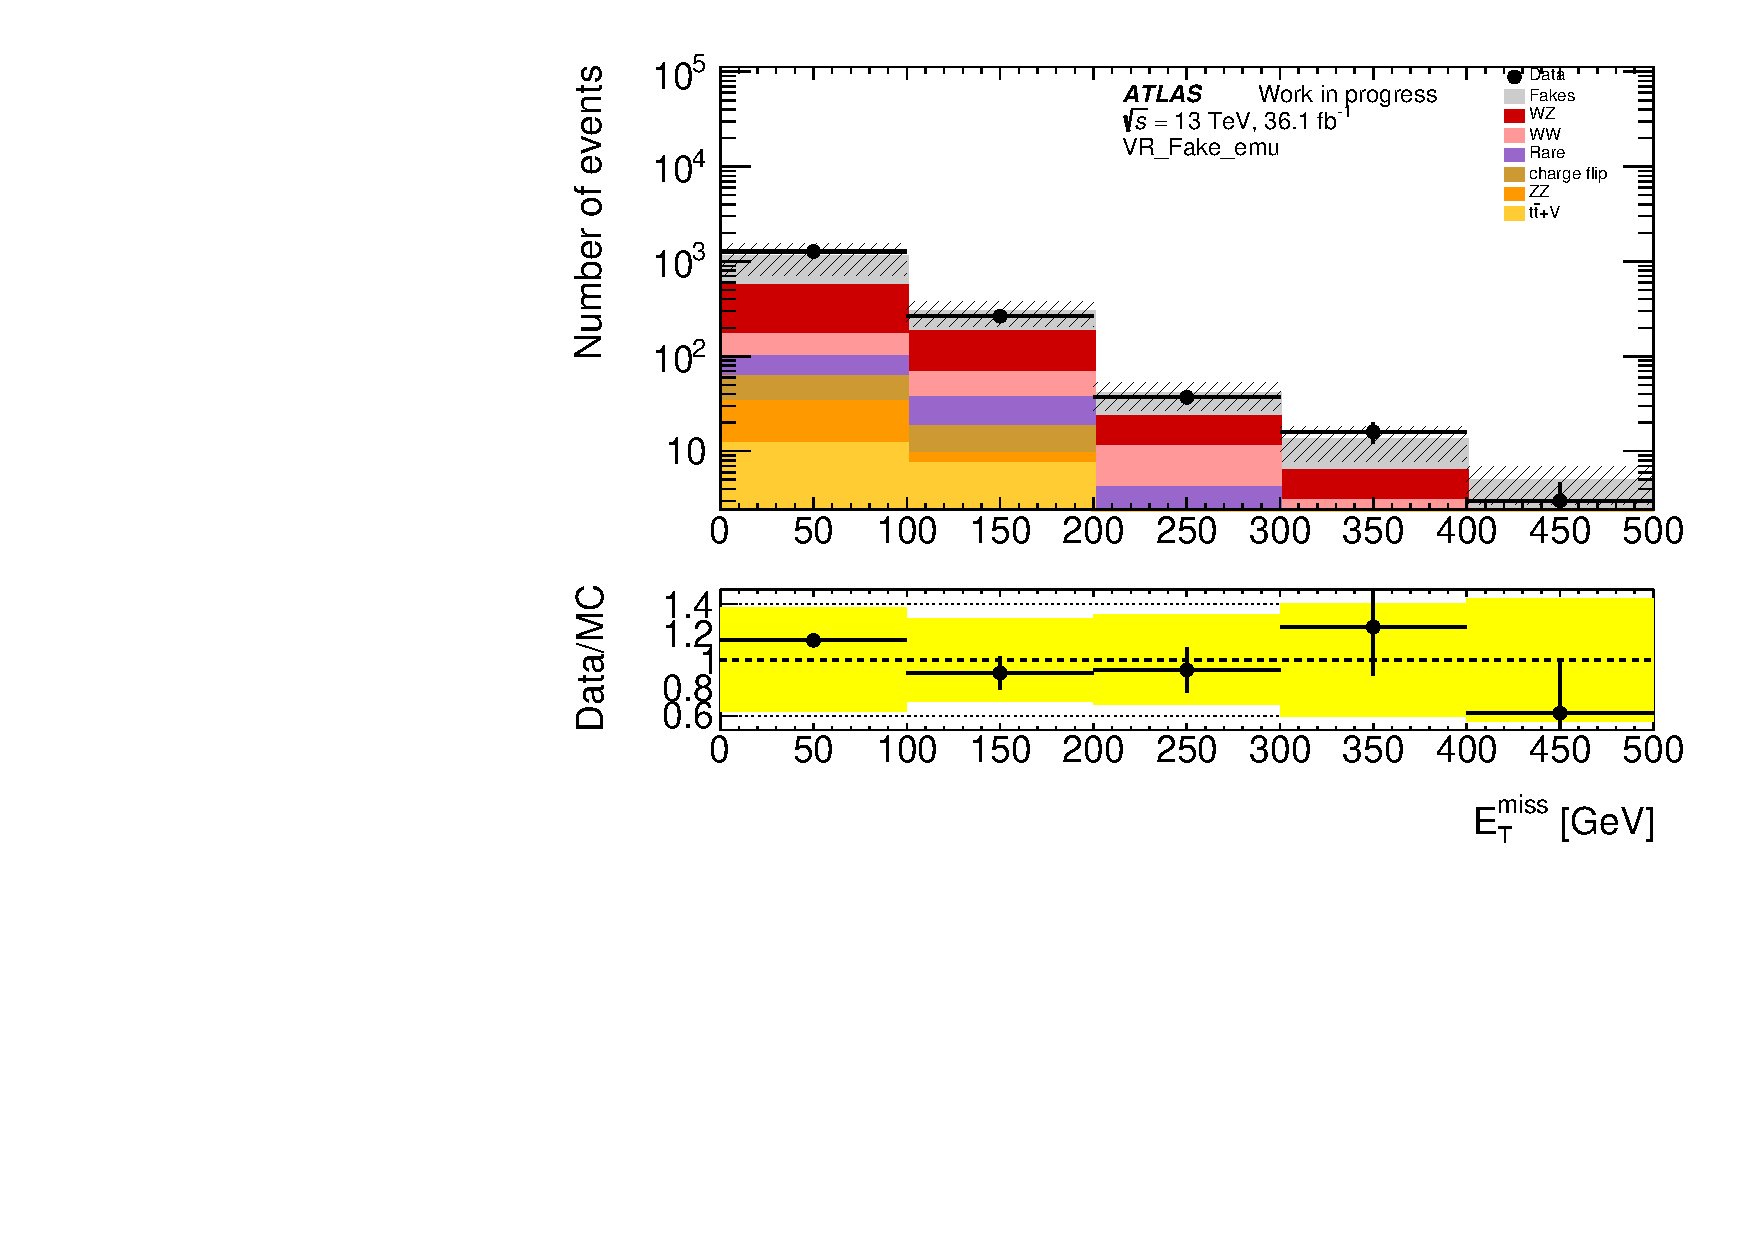
\includegraphics[width=0.49\textwidth]{data/plot/Fake_VR/MET_VR_Fake_emu}\\
\begin{center}
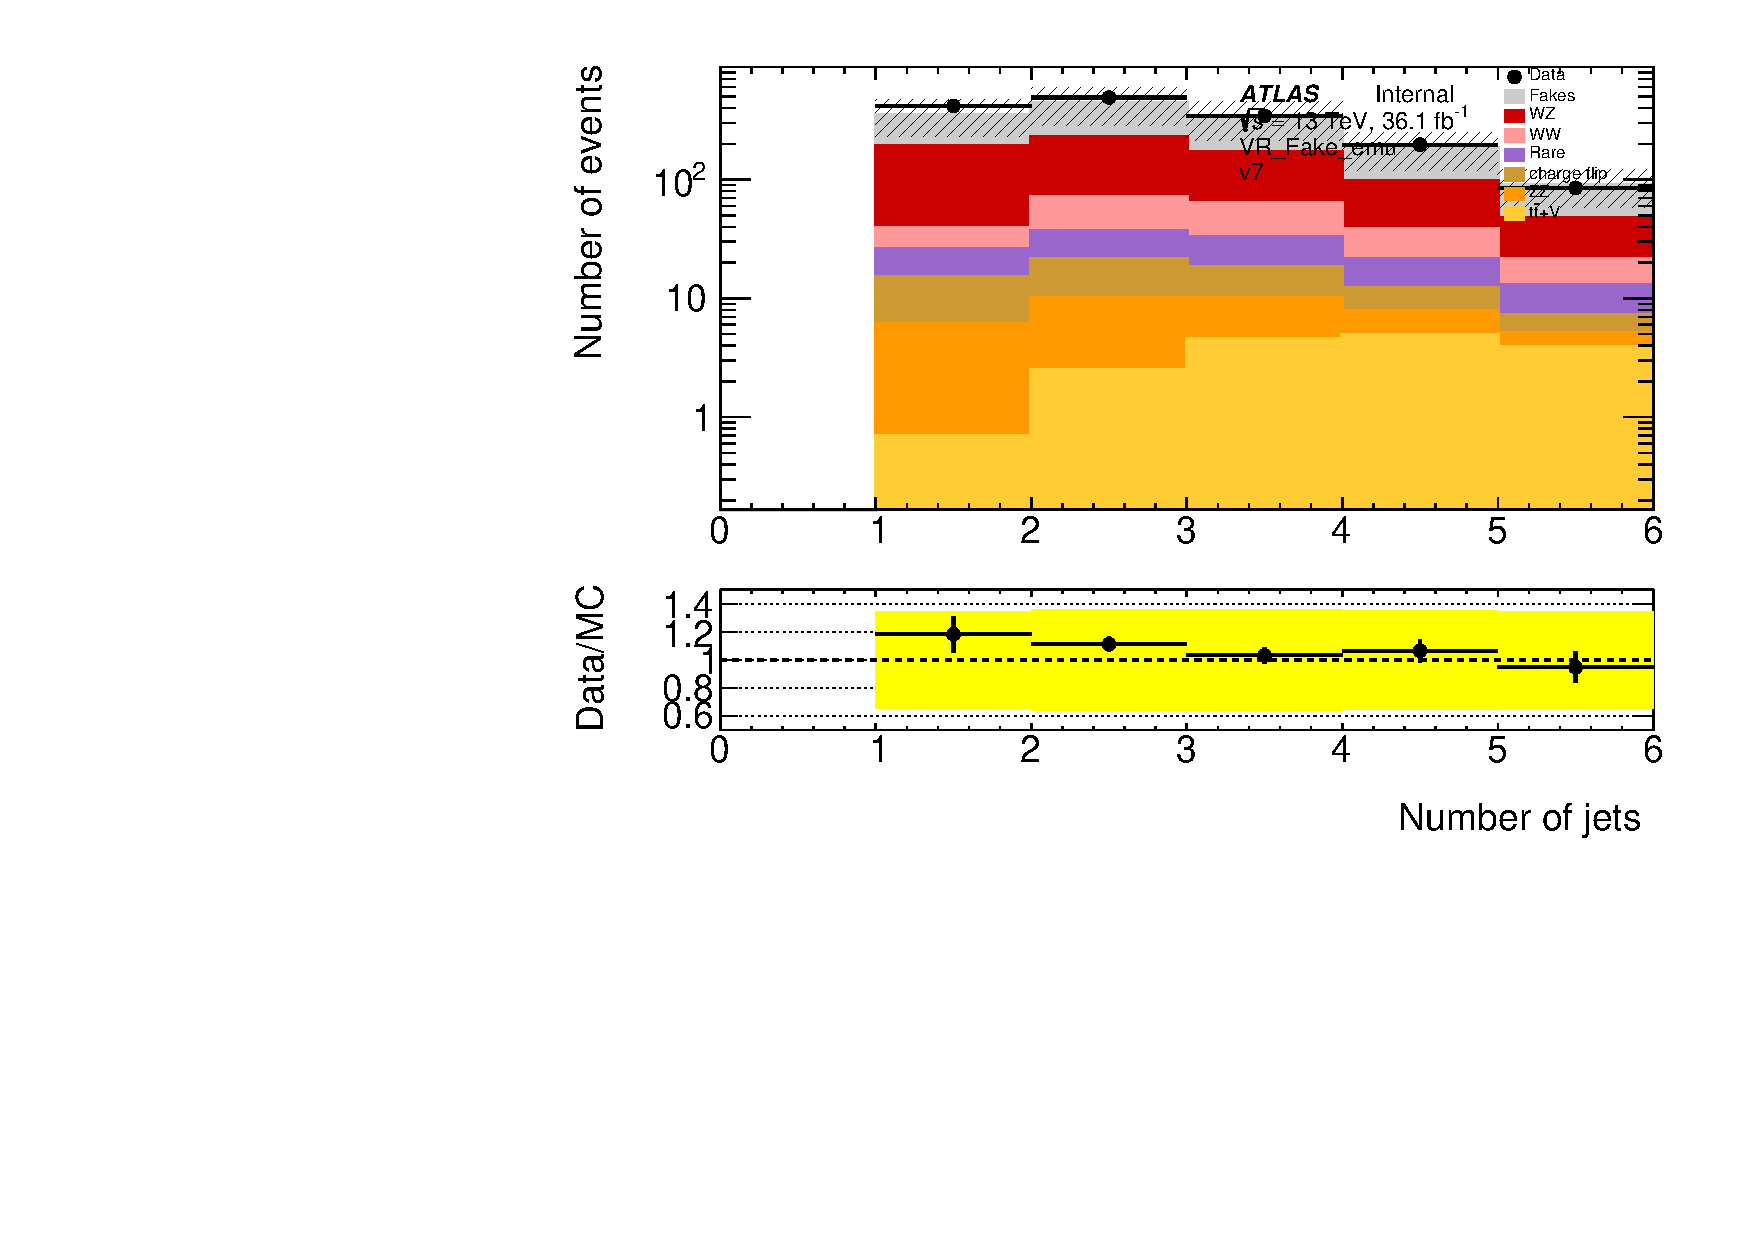
\includegraphics[width=0.49\textwidth]{data/plot/Fake_VR/nJet_VR_Fake_emu}
\end{center}
\caption{Distribution of the  leading lepton $p_T$, $m_{\text{eff}}$, $m_T$, $E_{T}^{\text{miss}}$ and $n_{\text{jets}}$ in the electron-muon channel. The ratio of data to background yields is shown in the lower plot. The error bar includes all the systematic uncertainties except for the theoretical uncertainties.}
\label{fig:VRSS_fake_emu}
\end{figure}
